% ==========================================
% IMPORT PREAMBLE - Cấu hình gói và định dạng
% ==========================================
% !TeX root = main.tex
\documentclass[12pt, a4paper]{project} % Dùng class tùy chỉnh có định nghĩa \coverpage và các biến trang bìa

% ==========================================
% 1. CÀI ĐẶT NGÔN NGỮ & FONT CHỮ
% ==========================================
\usepackage[T5]{fontenc}      % Hỗ trợ font tiếng Việt
\usepackage[utf8]{inputenc}   % Hỗ trợ gõ Unicode UTF-8
\usepackage[vietnamese]{babel} % Định dạng ngày tháng, tự động dịch các tiêu đề (Mục lục, Chương...)
\AtBeginDocument{\selectlanguage{vietnamese}}
\addto\captionsvietnamese{\renewcommand{\chaptername}{Chương}}

% Tăng cỡ chữ cho tiêu đề chương (vd: "Giới thiệu")
\makechapterstyle{nt531chapter}{
    \chapterstyle{default}
    \renewcommand{\chapnamefont}{\normalfont\Large\bfseries}
    \renewcommand{\chapnumfont}{\normalfont\Huge\bfseries}
    \renewcommand{\chaptitlefont}{\normalfont\Huge\bfseries}
}
\chapterstyle{nt531chapter}

% ==========================================
% 2. CĂN LỀ & ĐỊNH DẠNG TRANG
% ==========================================
\geometry{top=2.5cm, bottom=2.5cm, left=3cm, right=2cm} % Class đã load geometry, chỉ set lại thông số
\usepackage{fancyhdr}         % Tùy biến header/footer (đánh số trang)
\setlength{\parskip}{0.5em}   % Khoảng cách giữa các đoạn văn
\linespread{1.3}              % Dãn dòng 1.3 (tương đương 1.5 lines trong Word)

% ==========================================
% 3. XỬ LÝ BẢNG BIỂU (TABLES)
% ==========================================
\usepackage{tabularx}         % Tự động dàn trang bảng cho vừa chiều rộng
\usepackage{booktabs}         % Đường kẻ bảng chuyên nghiệp (toprule, midrule, bottomrule)
\usepackage{multirow}         % Gộp dòng (hữu ích cho bảng RQ/Fairness)
\usepackage{makecell}         % Cho phép ngắt dòng (enter) ngay trong 1 ô của bảng
\usepackage{longtable}        % Cho phép bảng tự động ngắt trang nếu quá dài (hữu ích cho Workloads table)

% ==========================================
% 4. XỬ LÝ HÌNH ẢNH & BIỂU ĐỒ (FIGURES)
% ==========================================
\usepackage{graphicx}         % Gói cơ bản để chèn ảnh
\usepackage{float}            % Ép vị trí ảnh bằng lệnh [H]
\usepackage{subcaption}       % Cho phép chèn nhiều ảnh nhỏ trong 1 ảnh lớn (VD: Đồ thị so sánh p99)

% ==========================================
% 5. CÔNG THỨC TOÁN HỌC & THỐNG KÊ
% ==========================================
\usepackage{amsmath, amssymb, amsfonts} % Hỗ trợ gõ công thức (p50, p99, O(1), O(n))

% ==========================================
% 6. MÃ NGUỒN & LOG (CODE & ARTIFACTS)
% ==========================================
\usepackage{listings}         % Chèn code (hữu ích cho manifests, bash script, hubble.log)
\usepackage{xcolor}           % Hỗ trợ tô màu cho code snippet

% Cấu hình mặc định cho khối code
\lstset{
    basicstyle=\ttfamily\small,
    breaklines=true,
    frame=single,
    backgroundcolor=\color{gray!10},
    keywordstyle=\color{blue},
    commentstyle=\color{green!50!black},
    stringstyle=\color{red}
}

% ==========================================
% 7. DANH SÁCH & LIÊN KẾT (LISTS & HYPERLINKS)
% ==========================================
\usepackage{enumitem}         % Tùy biến bullet points và numbering
\usepackage{hyperref}         % Class đã load hyperref; load lại không thêm options để tránh clash
\hypersetup{hidelinks}        % Ẩn viền link trong Mục lục/Danh mục
\usepackage{cleveref}         % Tham chiếu thông minh (tự động thêm chữ "Bảng", "Hình" trước số)

% ==========================================
% Chỉnh các biến cho phần trang bìa (cover page)
% Các biến này được định nghĩa trong file class project.cls
% ==========================================
\upperuniname{ĐẠI HỌC QUỐC GIA THÀNH PHỐ HỒ CHÍ MINH}
\uniname{TRƯỜNG ĐẠI HỌC CÔNG NGHỆ THÔNG TIN}
\deptname{KHOA MẠNG MÁY TÍNH VÀ TRUYỀN THÔNG}
\stumajor{KỸ SƯ NGÀNH MẠNG MÁY TÍNH VÀ TRUYỀN THÔNG DỮ LIỆU}
\coursename{ĐÁNH GIÁ HIỆU NĂNG\\HỆ THỐNG MẠNG MÁY TÍNH}
\coursecode{Mã môn: NT531.Q21}
\title{Đánh giá hiệu năng Kubernetes Service datapath giữa kube-proxy và Cilium eBPF kube-proxy replacement trên AWS EKS}
\titleen{TITLE FOR THE SPECIALIZED PROJECT IN ENGLISH}
\supervisor{GIẢNG VIÊN HƯỚNG DẪN}
\supervisorname{ThS. Đặng Lê Bảo chương}
\stunamewithid{Huỳnh Lê Đại Thắng - 23521422\\Bùi Ngọc Thái - 23521412\\Nguyễn Trường Duy - 23520380}
\reporttime{NĂM 2026}
\begin{document}
% ==========================================
% TRANG TIÊU ĐỀ & DANH MỤC
% ==========================================
\pagenumbering{gobble}
\coverpage

\pagenumbering{roman}
\setcounter{page}{1}

\tableofcontents    % Tự động tạo Mục lục 
\clearpage
\listoftables       % Tự động tạo Danh mục bảng 
\clearpage
\listoffigures      % Tự động tạo Danh mục hình 

\clearpage
\pagenumbering{arabic}
\setcounter{page}{1}

% Include các chương chính
% Chương 0: Phạm vi thực nghiệm + Chương 1: Introduction

% ==========================================
% CHƯƠNG 0: PHẠM VI THỰC NGHIỆM 
% ==========================================
\chapter*{Tóm tắt nội dung}

Đồ án \textit{``Đánh giá hiệu năng Kubernetes Service datapath giữa kube-proxy và Cilium eBPF kube-proxy replacement trên AWS EKS''} tập trung so sánh định lượng hiệu năng mạng giữa hai cơ chế: kiến trúc truyền thống dùng kube-proxy/iptables (duyệt luật tuần tự $O(n)$, phụ thuộc conntrack) và kiến trúc mới dùng Cilium eBPF (chuyển hướng trực tiếp ở cấp độ socket, tra cứu $O(1)$).

Các nội dung cốt lõi của đồ án được tóm tắt như sau:

\begin{enumerate}
\item \textbf{Mục tiêu và câu hỏi nghiên cứu.} Đồ án đặt ra ba câu hỏi chính nhằm lấp đầy khoảng trống nghiên cứu trên môi trường đám mây thực tế:
\begin{itemize}
	\item  \textbf{RQ1: }Ở trạng thái tải ổn định (steady-state), eBPF có cải thiện độ trễ phần đuôi (tail latency, đặc biệt là p99) so với kube-proxy hay không?
	\item  \textbf{RQ2: }Dưới mức tải cao đột biến (burst) và thay đổi kết nối liên tục (connection churn), hai chế độ xử lý khác nhau như thế nào?
	\item  \textbf{RQ3: }Mức hao tổn hiệu năng (overhead) là bao nhiêu khi bật NetworkPolicy kết hợp giám sát bằng Hubble trên eBPF?
\end{itemize}

\item \textbf{Thiết kế thực nghiệm (Methodology).}
\begin{itemize}
	\item \textbf{Môi trường:} Triển khai trên AWS EKS với 3 worker node loại m5.large. Client và Server được ép chạy cùng node để loại bỏ độ trễ mạng vật lý bên ngoài, tập trung vào lớp datapath.
	\item \textbf{Mức tải:} Sau hiệu chuẩn thực tế, chọn ba mức tải: L1 (100 QPS), L2 (400 QPS), L3 (800 QPS) -- trong đó L3 đủ tạo tail-spike nhưng chưa làm hệ thống sập.
	\item \textbf{Kịch bản:} S1 (tải tĩnh), S2 (tải biến động 4 pha: ramp-up, sustained, burst $\times 3$, cooldown với keep-alive tắt), S3 (so sánh policy OFF/ON trên mode eBPF).
	\item \textbf{Phân tích thống kê:} sử dụng Welch's t-test, p-value, khoảng tin cậy và phân tích độ lặp lại để tăng độ tin cậy cho kết luận.
\end{itemize}

\item \textbf{Kết quả nổi bật (Results \& Analysis).}
\begin{itemize}
	\item \textbf{S1 -- trả lời RQ1:} Mode B (eBPF) cải thiện p99 rõ ở tải trung bình và cao. Ở L3, p99 giảm khoảng 14.2\% so với kube-proxy, có ý nghĩa thống kê mạnh ($p=0.0191$).
	\item \textbf{S2 -- trả lời RQ2:} Kết quả phụ thuộc theo pha. Ở L3, Mode B có p99 trung bình thấp hơn ở tất cả các pha (có pha giảm đến 18.3\% ở Burst 1). Tuy nhiên, do variance cao của tải đột biến, kết luận phù hợp là ``xu hướng mạnh'' hơn là khẳng định ý nghĩa thống kê tuyệt đối cho từng pha đơn lẻ.
	\item \textbf{S3 -- trả lời RQ3:} Bật NetworkPolicy cơ bản trên eBPF tạo overhead rất nhỏ: p99 ở L3 chỉ chênh khoảng +1.2\%, RPS gần như không đổi và error rate giữ 0\%. Điều này cho thấy cơ chế policy enforcement trên eBPF hiệu quả và ít ảnh hưởng hiệu năng trong setup hiện tại.
\end{itemize}

\item \textbf{Kết luận và giới hạn.}
\begin{itemize}
	\item \textbf{Kết luận:} eBPF là lựa chọn hiệu quả để giảm tail latency, phù hợp với các hệ thống microservices có tải trung bình đến cao và nhạy cảm SLA.
	\item \textbf{Giới hạn:} Nghiên cứu tập trung vào ClusterIP nội node, workload tổng hợp HTTP (Fortio), và policy tương đối đơn giản; do đó kết quả chưa đại diện cho mọi kịch bản traffic phức tạp ngoài thực tế.
\end{itemize}
\end{enumerate}

\clearpage

% ==========================================
% CHƯƠNG 1: INTRODUCTION 
% ==========================================
\chapter{Giới thiệu}
\section{Bối cảnh nghiên cứu} %
 Kubernetes hiện đang là tiêu chuẩn thực tế trong việc điều phối container, nơi mà lớp mạng đóng vai trò quyết định đối với độ trễ của các dịch vụ. 
 Theo mặc định, thành phần kube-proxy trong Kubernetes chịu trách nhiệm hiện thực hóa cơ chế định tuyến dịch vụ (như ClusterIP) bằng cách sử dụng iptables 
 hoặc ipvs. Tuy nhiên, iptables bộc lộ một điểm nghẽn lớn: nó sử dụng cơ chế duyệt tuần tự các chuỗi luật với độ phức tạp O(n), khiến thời gian tra cứu 
 tăng tuyến tính khi số lượng service trong cụm ngày càng nhiều. Để giải quyết vấn đề này, công nghệ Cilium cung cấp một giải pháp thay thế hoàn toàn 
 kube-proxy bằng cách sử dụng eBPF (kube-proxy replacement), nhằm giảm suy hao hệ thống và cải thiện độ trễ phần đuôi nhờ cơ chế tra cứu bảng băm (BPF maps) 
 với thời gian cố định O(1).
\section{Vấn đề nghiên cứu} % 
Mặc dù giải pháp Cilium eBPF có lợi thế rõ ràng về mặt lý thuyết, bối cảnh nghiên cứu hiện tại đang tồn tại một khoảng trống nghiên cứu lớn. 
Các bài đánh giá hiệu năng hiện có chủ yếu được thực hiện trong môi trường giả lập (Minikube/local), máy chủ vật lý (bare-metal) hoặc GKE, thiếu đi những bằng chứng thực nghiệm trên các cụm triển khai chuẩn sản xuất (production-grade cluster) như AWS EKS. 
Bên cạnh đó, các nghiên cứu này cũng thiếu sự đánh giá định lượng có kiểm soát về mặt thống kê, chẳng hạn khoảng tin cậy, kiểm định kiểu Welch và phân tích độ lặp lại; thiếu các phân tích ở cấp độ 
từng giai đoạn (phase-level) khi hệ thống chịu tải đột biến; và chưa đánh giá đầy đủ mức hao tổn khi áp dụng các chính sách mạng (NetworkPolicy) kèm bằng chứng quan sát phù hợp.
\section{Mục tiêu nghiên cứu} % 
\subsection{Mục tiêu chính}
Đánh giá định lượng và so sánh hiệu năng của đường dẫn mạng Kubernetes Service (datapath) giữa hai cơ chế: Mode A (kube-proxy baseline) và Mode B 
(Cilium eBPF kube-proxy replacement) trên nền tảng điện toán đám mây AWS EKS thực tế.

\subsection{Mục tiêu cụ thể}
\begin{enumerate}
\item Đo lường xem Mode B có giúp cải thiện độ trễ phần đuôi (tail latency - đặc biệt là p99, với p50/p90 làm chỉ số bổ trợ) so với Mode A ở điều kiện tải ổn định (steady-state) hay không.
\item Đánh giá tính ổn định của luồng mạng (tỷ lệ lỗi, độ trễ gai) dưới mức tải cao và sự thay đổi kết nối liên tục (connection churn).
\item Đo lường mức độ hao tổn hiệu năng (overhead) tác động lên thông lượng và độ trễ khi bật các quy tắc mạng (NetworkPolicy) kết hợp với công cụ quan sát Hubble.
Các mục tiêu cụ thể này cũng sẽ là 3 câu hỏi nghiên cứu (Research questions - RQ). Mỗi kịch bản đo lường được đặt ra để thu thập các dữ liệu phục vụ cho việc trả lời các câu hỏi đó.
\end{enumerate}
% Chèn Table 3.3 RQ to Metric Traceability tại đây 
\section{Phạm vi nghiên cứu} % 
\subsection{Phạm vi đo lường} % 
Tập trung đo lường luồng traffic nội bộ (east-west) qua Service kiểu ClusterIP. Các Pod client và server được ép chạy trên cùng một node (same-node placement) 
để giảm nhiễu độ trễ từ mạng vật lý liên node/liên vùng, qua đó tập trung hơn vào khác biệt của service datapath. Benchmark không bao gồm traffic kết nối ra Internet, 
traffic liên cụm (multi-cluster), hay streaming dữ liệu lớn.
\subsection{Cấu hình phần cứng thực nghiệm}
Triển khai 01 cụm Kubernetes trên AWS EKS (phiên bản 1.34) và Cilium (phiên bản 1.18.7) tại region ap-southeast-1. Cụm sử dụng 3 worker nodes loại m5.large 
(non-burstable CPU để tránh cạn kiệt CPU credit làm nhiễu kết quả) và được ghim vào một Availability Zone (AZ) duy nhất. Chức năng autoscaling bị tắt 
trong quá trình đo đạc để giữ cố định số lượng node.
\subsection{Ý nghĩa của nghiên cứu} % 
Cung cấp các bằng chứng thực nghiệm đáng tin cậy và có ý nghĩa thống kê cho các hệ thống chuẩn sản xuất. Nghiên cứu đưa ra hệ quả thực tiễn 
giúp các kỹ sư ra quyết định chuyển đổi sang eBPF KPR, đặc biệt phù hợp cho các cụm có quy mô lớn, các hệ thống 
nhạy cảm với độ trễ bị ràng buộc bởi SLA (p99/p999), hoặc khi cần quan sát luồng ở mức flow-level và kiểm chứng thực thi NetworkPolicy bằng Hubble. Trong phạm vi đề tài, Hubble đóng vai trò cung cấp evidence về flow và verdict để hỗ trợ đối chiếu hành vi policy, không thay thế các số liệu hiệu năng chính như latency, RPS và error rate. Đồng thời, nghiên cứu cũng cảnh báo các rủi ro 
vận hành như xung đột bảng NAT nếu không tắt kube-proxy đúng cách trước khi chuyển đổi.

% Chương 2: Background & Related Work

% ==========================================
% CHƯƠNG 2: BACKGROUND & RELATED WORK
% ==========================================
\chapter{Cơ sở lý thuyết}

Chương này trình bày kiến thức nền và công trình liên quan phục vụ cho phần thiết kế thực nghiệm ở các chương sau. Nội dung chương tập trung vào cơ chế và khái niệm, không đi sâu vào kết quả đo của hệ thống cụ thể.

\section{Cơ chế xử lý gói tin trong nhân Linux}
Trong Linux networking stack, gói tin đi qua nhiều tầng xử lý trước khi tới ứng dụng đích. Với bối cảnh Kubernetes Service 
datapath, các khái niệm nền tảng cần nắm gồm:
\subsection{Netfilter framework/ iptables và chains} iptables là công cụ cấu hình mạng hoạt động trong nhân Linux, xử lý gói tin bằng cách cho chúng đi qua các chuỗi (chains) cơ bản như PREROUTING, INPUT, OUTPUT, FORWARD, và POSTROUTING. Trong Kubernetes, kube-proxy sẽ tạo ra các chuỗi tùy chỉnh như KUBE-SERVICES (để nhận diện IP của Service) và KUBE-SEP-* (để chọn endpoint cụ thể). Quá trình tra cứu các luật (rules) trong iptables diễn ra tuần tự (linear scan), tạo ra độ phức tạp O(n). Khi có hàng ngàn Service, số lượng luật tăng lên hàng chục nghìn, khiến thời gian duyệt tăng tuyến tính và gây ra thắt cổ chai.
\subsection{DNAT và SNAT (Network Address Translation)} 
\begin{itemize}
	\item \textbf{DNAT (Destination NAT):} Khi một gói tin được gửi đến địa chỉ ảo của Service (ClusterIP), chuỗi PREROUTING sẽ áp dụng DNAT để biến đổi địa chỉ IP đích từ Service IP sang địa chỉ IP thực của một Pod backend.
	\item SNAT (Source NAT / Masquerade): Khi gói tin đi ra khỏi Pod hoặc Node, chuỗi POSTROUTING sẽ thực hiện SNAT, thay đổi địa chỉ IP nguồn từ IP của Pod thành IP của Node vật lý để che giấu (hide) địa chỉ IP nội bộ của Pod.
\end{itemize}
\subsection{Conntrack (Connection Tracking)}
Đây là một hệ thống con (subsystem) của kernel chuyên theo dõi trạng thái của các kết nối mạng (stateful inspection). Ví dụ, một gói tin TCP SYN tạo ra trạng thái NEW, và gói SYN-ACK cập nhật trạng thái thành ESTABLISHED. Bất kỳ thao tác NAT nào cũng bắt buộc phải có conntrack để ghi nhớ IP/Port gốc, từ đó giúp kernel có thể dịch ngược lại chính xác địa chỉ cho các gói tin phản hồi (reply traffic). Điểm yếu của cơ chế này là dưới mức tải cao, nếu bảng conntrack đạt đến giới hạn tối đa (bị đầy), hệ thống sẽ từ chối (DROP) các kết nối mới làm thông lượng mạng sụt giảm đột ngột.


Trong benchmark networking, tail latency thường nhạy với độ phức tạp đường đi gói tin và mức tải của các thành phần xử lý trạng thái như conntrack. Vì vậy, khi phân tích p95/p99 cần đặt kết quả trong ngữ cảnh đường đi datapath thực tế.

\section{Kubernetes networking background}
Tại mức khái niệm, Service trong Kubernetes cung cấp một virtual IP (ClusterIP) để phân phối traffic tới tập backend endpoints. kube-proxy thường đảm nhiệm phần điều hướng Service bằng cách lập trình luật iptables hoặc cơ chế tương đương.

Trong khi đó, CNI chịu trách nhiệm kết nối mạng cho Pod và thiết lập các thành phần dữ liệu cần thiết cho dataplane. Cilium là một CNI dựa trên eBPF, cho phép đưa một phần logic xử lý gói tin xuống kernel theo hướng lập trình được, đồng thời cung cấp khả năng quan sát luồng mạng (flow observability).

Khái niệm kube-proxy replacement của Cilium trong nghiên cứu này được hiểu là thay thế phần xử lý Service forwarding của kube-proxy bằng datapath eBPF tương ứng.

\section{Datapath comparison at concept level}
Ở mức ý niệm, hai mode được đối chiếu theo các đường đi điển hình sau:

\textbf{Mode A (kube-proxy baseline)}
\begin{itemize}
	\item client $\rightarrow$ veth $\rightarrow$ host netns $\rightarrow$ iptables/kube-proxy path $\rightarrow$ endpoint.
\end{itemize}

\textbf{Mode B (Cilium eBPF kube-proxy replacement)}
\begin{itemize}
	\item client $\rightarrow$ veth $\rightarrow$ TC eBPF $\rightarrow$ service map $\rightarrow$ endpoint/policy map.
\end{itemize}

Trong phạm vi chương này, phần so sánh chỉ nhằm mô tả background mechanism. Nghiên cứu không đưa ra tuyên bố độ phức tạp thuật toán theo dạng chứng minh hình thức.

\begin{figure}[H]
\centering
\begin{tikzpicture}[x=1cm,y=1cm]
	% Khung tổng thể
	\draw[rounded corners=2pt] (-0.2,-0.4) rectangle (14.2,5.8);
	\draw (7,-0.4) -- (7,5.8);

	% Tieu de hai cot
	\node[font=\bfseries] at (3.5,5.2) {Mode A: kube-proxy (iptables)};
	\node[font=\bfseries] at (10.5,5.2) {Mode B: Cilium eBPF KPR};

	% Mode A
	\draw[rounded corners=2pt] (0.6,3.7) rectangle (2.8,4.5);
	\node at (1.7,4.1) {Client Pod};
	\draw[rounded corners=2pt] (3.4,3.7) rectangle (5.8,4.5);
	\node at (4.6,4.1) {veth/host netns};
	\draw[rounded corners=2pt] (0.6,2.2) rectangle (2.8,3.0);
	\node at (1.7,2.6) {kube-proxy};
	\draw[rounded corners=2pt] (3.4,2.2) rectangle (5.8,3.0);
	\node at (4.6,2.6) {DNAT/SNAT};
	\draw[rounded corners=2pt] (2.0,0.8) rectangle (4.4,1.6);
	\node at (3.2,1.2) {Server Pod};

	\draw[->,thick] (2.8,4.1) -- (3.4,4.1);
	\draw[->,thick] (1.7,3.7) -- (1.7,3.0);
	\draw[->,thick] (2.8,2.6) -- (3.4,2.6);
	\draw[->,thick] (4.6,2.2) -- (3.5,1.6);

	% Mode B
	\draw[rounded corners=2pt] (7.6,3.7) rectangle (9.8,4.5);
	\node at (8.7,4.1) {Client Pod};
	\draw[rounded corners=2pt] (10.4,3.7) rectangle (12.8,4.5);
	\node at (11.6,4.1) {veth/TC hook};
	\draw[rounded corners=2pt] (7.6,2.2) rectangle (9.8,3.0);
	\node at (8.7,2.6) {eBPF prog};
	\draw[rounded corners=2pt] (10.4,2.2) rectangle (12.8,3.0);
	\node at (11.6,2.6) {BPF service/policy maps};
	\draw[rounded corners=2pt] (9.0,0.8) rectangle (11.4,1.6);
	\node at (10.2,1.2) {Server Pod};

	\draw[->,thick] (9.8,4.1) -- (10.4,4.1);
	\draw[->,thick] (8.7,3.7) -- (8.7,3.0);
	\draw[->,thick] (9.8,2.6) -- (10.4,2.6);
	\draw[->,thick] (11.6,2.2) -- (10.5,1.6);
\end{tikzpicture}
\caption{Datapath Comparison Diagram (conceptual)}
\label{fig:datapath-comparison}
\end{figure}

\section{Hubble and policy observability}
Hubble cung cấp mặt quan sát flow-level cho môi trường Cilium, bao gồm các thông tin như quan hệ nguồn-đích, metadata ngữ cảnh, và verdict của flow. Trong thesis này, Hubble được sử dụng như nguồn evidence bổ trợ thay vì thay thế số đo hiệu năng từ workload benchmark.

Các trạng thái verdict điển hình gồm \texttt{FORWARDED}/\texttt{DROPPED} và \texttt{ALLOWED}/\texttt{DENIED}. Vai trò chính của Hubble trong nghiên cứu là:
\begin{itemize}
	\item supporting evidence cho tính đúng đắn của đường đi traffic.
	\item correctness evidence khi kiểm chứng hành vi policy.
	\item bằng chứng đặc biệt quan trọng cho kịch bản S3 (policy overhead).
\end{itemize}

\section{Related work}
Tổng quan công trình liên quan được tóm tắt ở Bảng~\ref{tab:related-work-comparison}. Bảng này tập trung vào khoảng trống giữa tài liệu kỹ thuật hiện có và nhu cầu benchmark thực nghiệm có kiểm soát trên EKS.

\begin{table}[H]
\centering
\caption{Related Work Comparison}
\label{tab:related-work-comparison}
\begin{tabularx}{\textwidth}{>{\raggedright\arraybackslash}p{2.5cm}>{\raggedright\arraybackslash}p{1.9cm}X>{\raggedright\arraybackslash}p{2.8cm}>{\raggedright\arraybackslash}p{3.0cm}}
\toprule
\textbf{Nguồn} & \textbf{Môi trường} & \textbf{Nội dung chính} & \textbf{Điểm còn thiếu} & \textbf{Thesis này bổ sung} \\
\midrule
Cilium docs/benchmark notes & self-managed/cloud & Benchmark về Cilium và cơ chế datapath & Thiếu protocol đầy đủ và bộ artifact chuẩn hóa & Protocol benchmark rõ ràng, artifact provenance nhất quán \\
Kubernetes/kube-proxy docs & docs & Mô tả cơ chế Service handling và kube-proxy & Không có benchmark so sánh A/B đầy đủ trên EKS & Benchmark A/B trực tiếp trên EKS thật \\
Tài liệu Hubble & docs & Flow observability và policy verdict & Không đo policy overhead dưới workload thực nghiệm & Bổ sung S3 policy overhead kèm evidence theo flow \\
Các nguồn blog/notes cộng đồng & mixed & Kinh nghiệm thực hành và tuning thực tế & Khó tái lập, thiếu kiểm soát biến & Thiết kế thực nghiệm kiểm soát biến và phạm vi kết luận rõ ràng \\
\bottomrule
\end{tabularx}
\end{table}

\section{Scope boundary}
Để tránh over-claim, thesis xác định rõ biên phạm vi của kết luận như sau.

\textbf{Trong scope}
\begin{itemize}
	\item Service kiểu \texttt{ClusterIP}.
	\item Workload HTTP.
	\item Ưu tiên same-node theo thiết kế triển khai benchmark.
	\item Các kịch bản S1, S2, S3 như định nghĩa trong protocol.
\end{itemize}

\textbf{Ngoài scope}
\begin{itemize}
	\item Nghiên cứu đầy đủ cross-node path ở quy mô mở rộng.
	\item Service kiểu NodePort/LoadBalancer.
	\item Workload gRPC.
	\item Policy complexity scaling nhiều cấp độ.
	\item Môi trường multi-cluster.
\end{itemize}

% Chương 3: System Design & Methodology

% ==========================================
% CHƯƠNG 3: SYSTEM DESIGN & METHODOLOGY 
% ==========================================
\chapter{System Design, Implementation \& Methodology}
\section{System overview} % 
% Chèn Table 3.1 Infrastructure Specifications tại đây 
\section{Deployment topology} % 
% Chèn Figure 3.1 EKS Deployment Topology tại đây 
\section{Mode definitions} % 
\section{Fairness giữa hai mode} % 
\section{Workload and toolchain} % 
% Chèn Table 3.2 Workload Configuration tại đây 
\section{Code analysis / tracing / logging} % 
\section{Experimental design} % 
\section{Load calibration} % 
\section{Run protocol} % 
\section{Scenarios (S1, S2, S3)} % 
\section{Statistics plan} % 
\section{Fairness controls} % 
\section{Threats to validity} % 

% !TeX root = ../../main.tex
% Chương 4: Kết quả và Phân tích

\chapter{Kết quả và Phân tích}

Chương này trình bày kết quả benchmark theo từng kịch bản đã mô tả ở Chương 3. Mạch phân tích bắt đầu từ kịch bản đo và mức tải, sau đó đọc kết quả, diễn giải xu hướng và rút ra kết luận. Các bảng và biểu đồ là kết quả hậu xử lý từ các lần chạy benchmark, giúp việc đọc kết quả có hệ thống hơn.

Trọng tâm của chương là trả lời ba câu hỏi: mỗi kịch bản kiểm tra điều gì, kết quả chính là gì và có thể kết luận đến mức nào. Các thống kê như khoảng tin cậy 95\%, delta \%, giá trị \(p\) theo kiểm định kiểu Welch và CV\% được dùng như bằng chứng hỗ trợ.

Trong chương này, một kết quả được xem là có ý nghĩa thống kê khi \(p < 0.05\), tức là dữ liệu hiện tại đủ mạnh để bác bỏ giả thuyết không \(H_0\) ở mức ý nghĩa 5\%. Với so sánh A/B, \(H_0\) được hiểu là hai nhóm không khác biệt đáng kể về trung bình của metric đang xét. Tuy nhiên, do nhiều nhóm đo chỉ có \(n=3\), ý nghĩa thống kê chỉ được dùng như bằng chứng hỗ trợ và phải đọc cùng delta \%, khoảng tin cậy 95\% và bối cảnh kịch bản.

\section{Hiệu chuẩn tải và lựa chọn mức tải}

Hiệu chuẩn tải được thực hiện trước benchmark chính để chọn các mức tải phù hợp. Nếu tải quá thấp, khác biệt giữa hai mode có thể bị che khuất. Nếu tải quá cao, kết quả có thể bị chi phối bởi stress cực đoan. Vì vậy, L1, L2 và L3 được chọn từ dữ liệu hiệu chuẩn thay vì chọn thủ công.

Hình~\ref{fig:calibration-curve} biểu diễn p99 latency theo target QPS trong lượt quét hiệu chuẩn. P99 được dùng vì phần đuôi độ trễ thường nhạy hơn với queueing, scheduling, connection handling và chi phí xử lý Service. Các đường dọc trong hình chỉ đánh dấu L1, L2 và L3; chúng không phải error bars.

\begin{figure}[H]
    \centering
    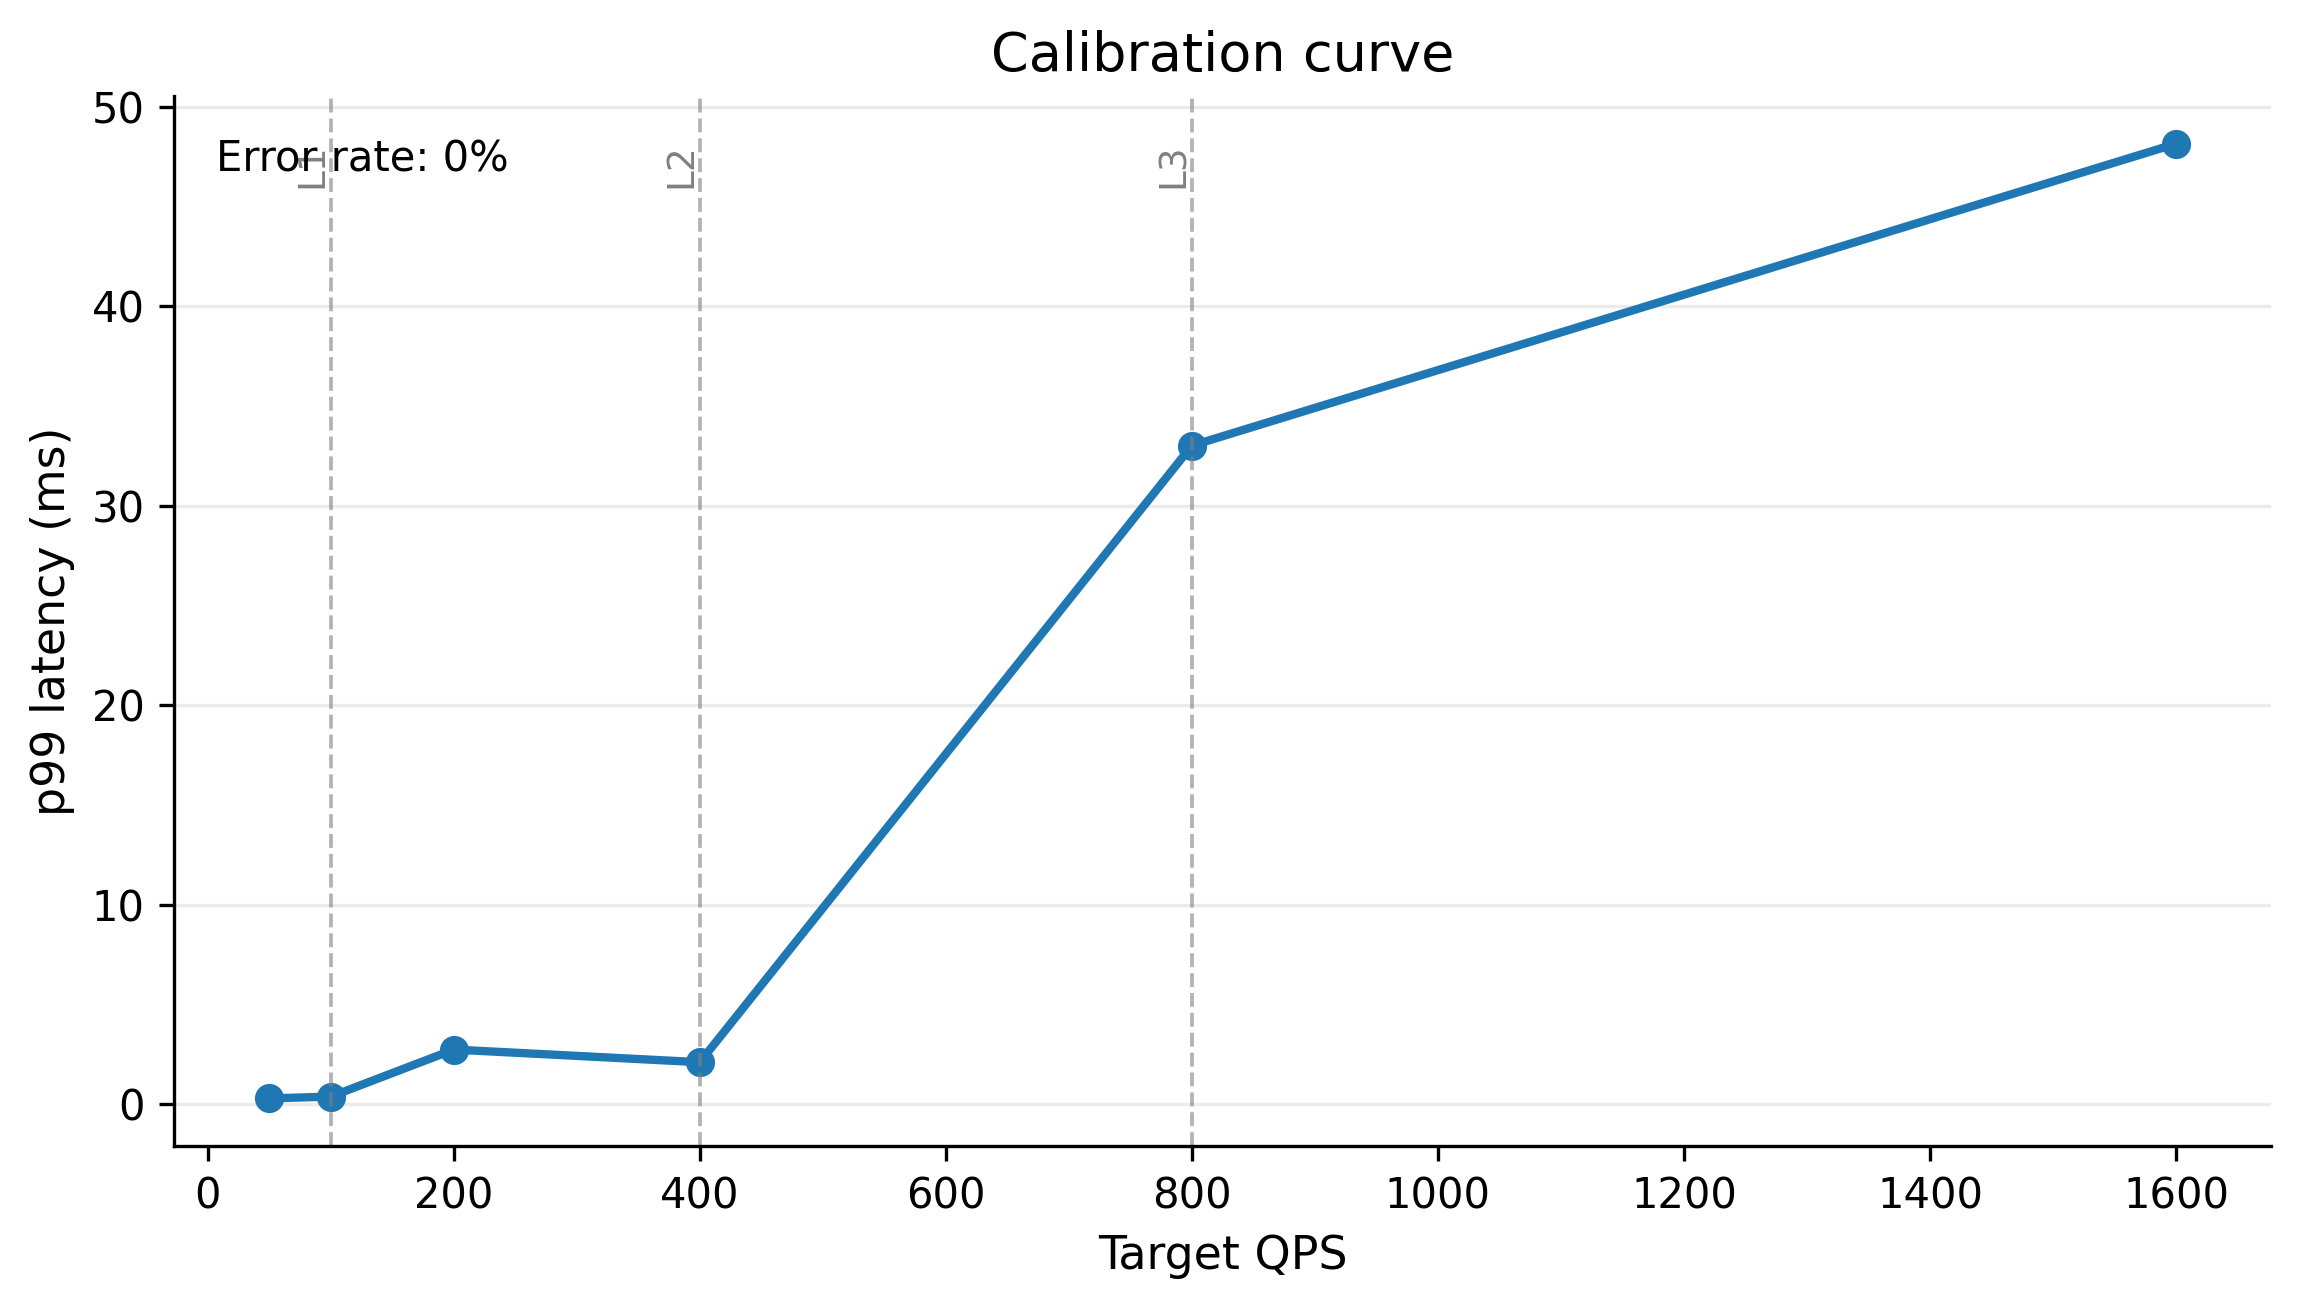
\includegraphics[width=0.90\textwidth]{../figures/thesis/fig-calibration-curve.png}
    \caption{Đường hiệu chuẩn tải và lựa chọn L1, L2, L3; các đường dọc chỉ là mốc tải, không phải thanh sai số}
    \label{fig:calibration-curve}
\end{figure}

\begin{table}[H]
\centering
\caption{Tóm tắt các điểm hiệu chuẩn tải}
\label{tab:calibration-load-selection}
\renewcommand{\arraystretch}{1.2}
\begin{tabularx}{\textwidth}{>{\raggedleft\arraybackslash}p{1.2cm}>{\raggedleft\arraybackslash}p{1.3cm}>{\raggedleft\arraybackslash}p{1.5cm}>{\raggedleft\arraybackslash}p{1.5cm}>{\raggedleft\arraybackslash}p{1.7cm}>{\raggedleft\arraybackslash}p{1.7cm}>{\raggedright\arraybackslash}X}
\toprule
\textbf{QPS} & \textbf{Conns} & \textbf{p50} & \textbf{p90} & \textbf{p99} & \textbf{Lỗi} & \textbf{Vai trò} \\
\midrule
100 & 8 & 0.208 ms & 0.353 ms & 0.385 ms & 0.000\% & L1, tải nhẹ \\
400 & 32 & 0.846 ms & 1.854 ms & 2.107 ms & 0.000\% & L2, tải trung bình \\
800 & 64 & 1.709 ms & 4.411 ms & 33.006 ms & 0.000\% & L3, tải cao có p99 tăng rõ \\
1600 & 64 & 3.085 ms & 5.746 ms & 48.135 ms & 0.000\% & Điểm stress cao hơn, không dùng làm L3 cuối \\
\bottomrule
\end{tabularx}
\end{table}

\textbf{Phân tích.} Kết quả hiệu chuẩn cho thấy 100 QPS phù hợp làm L1 vì p99 thấp và ổn định. Mức 400 QPS được chọn làm L2 vì tail latency bắt đầu rõ hơn nhưng chưa tạo lỗi HTTP. Mức 800 QPS được chọn làm L3 vì p99 tăng mạnh lên khoảng 33.006 ms, trong khi achieved RPS vẫn gần target và error rate vẫn bằng 0\%.

Như vậy, 800 QPS đủ làm phần đuôi độ trễ nhạy hơn mà chưa biến phép đo thành tình huống lỗi hàng loạt. Điểm 1600 QPS không được chọn làm L3 vì có thể làm các pha burst của S2 quá cực đoan. Do đó, L3 nên được hiểu là mức tải cao làm lộ rõ tail latency, không phải điểm bão hòa tuyệt đối.

\textbf{Kết luận.} Error rate bằng 0\% chỉ cho thấy request không lỗi HTTP trong phạm vi đo; nó không có nghĩa hệ thống không chịu áp lực. Sự tăng mạnh của p99 tại 800 QPS là cơ sở để xem L3 là mức tải cao có ý nghĩa phân tích. Vì vậy, L1/L2/L3 phù hợp để dùng cho benchmark chính.

\section{Kết quả S1: tải ổn định}

S1 so sánh Mode A và Mode B trong điều kiện service traffic ổn định. Đây là kịch bản sạch nhất để quan sát khác biệt datapath vì không có burst, không thay đổi policy OFF/ON và không cố ý tạo connection churn. Metric chính là p99 latency vì benchmark tập trung vào tail latency.

Các biểu đồ chính của S1 gồm p99 theo mức tải, so sánh p50/p90/p99 và delta p99 của Mode B so với Mode A. Ba hình này lần lượt cho biết xu hướng tail latency, xu hướng ở nhiều percentile và độ lớn chênh lệch theo phần trăm.

\begin{figure}[H]
    \centering
    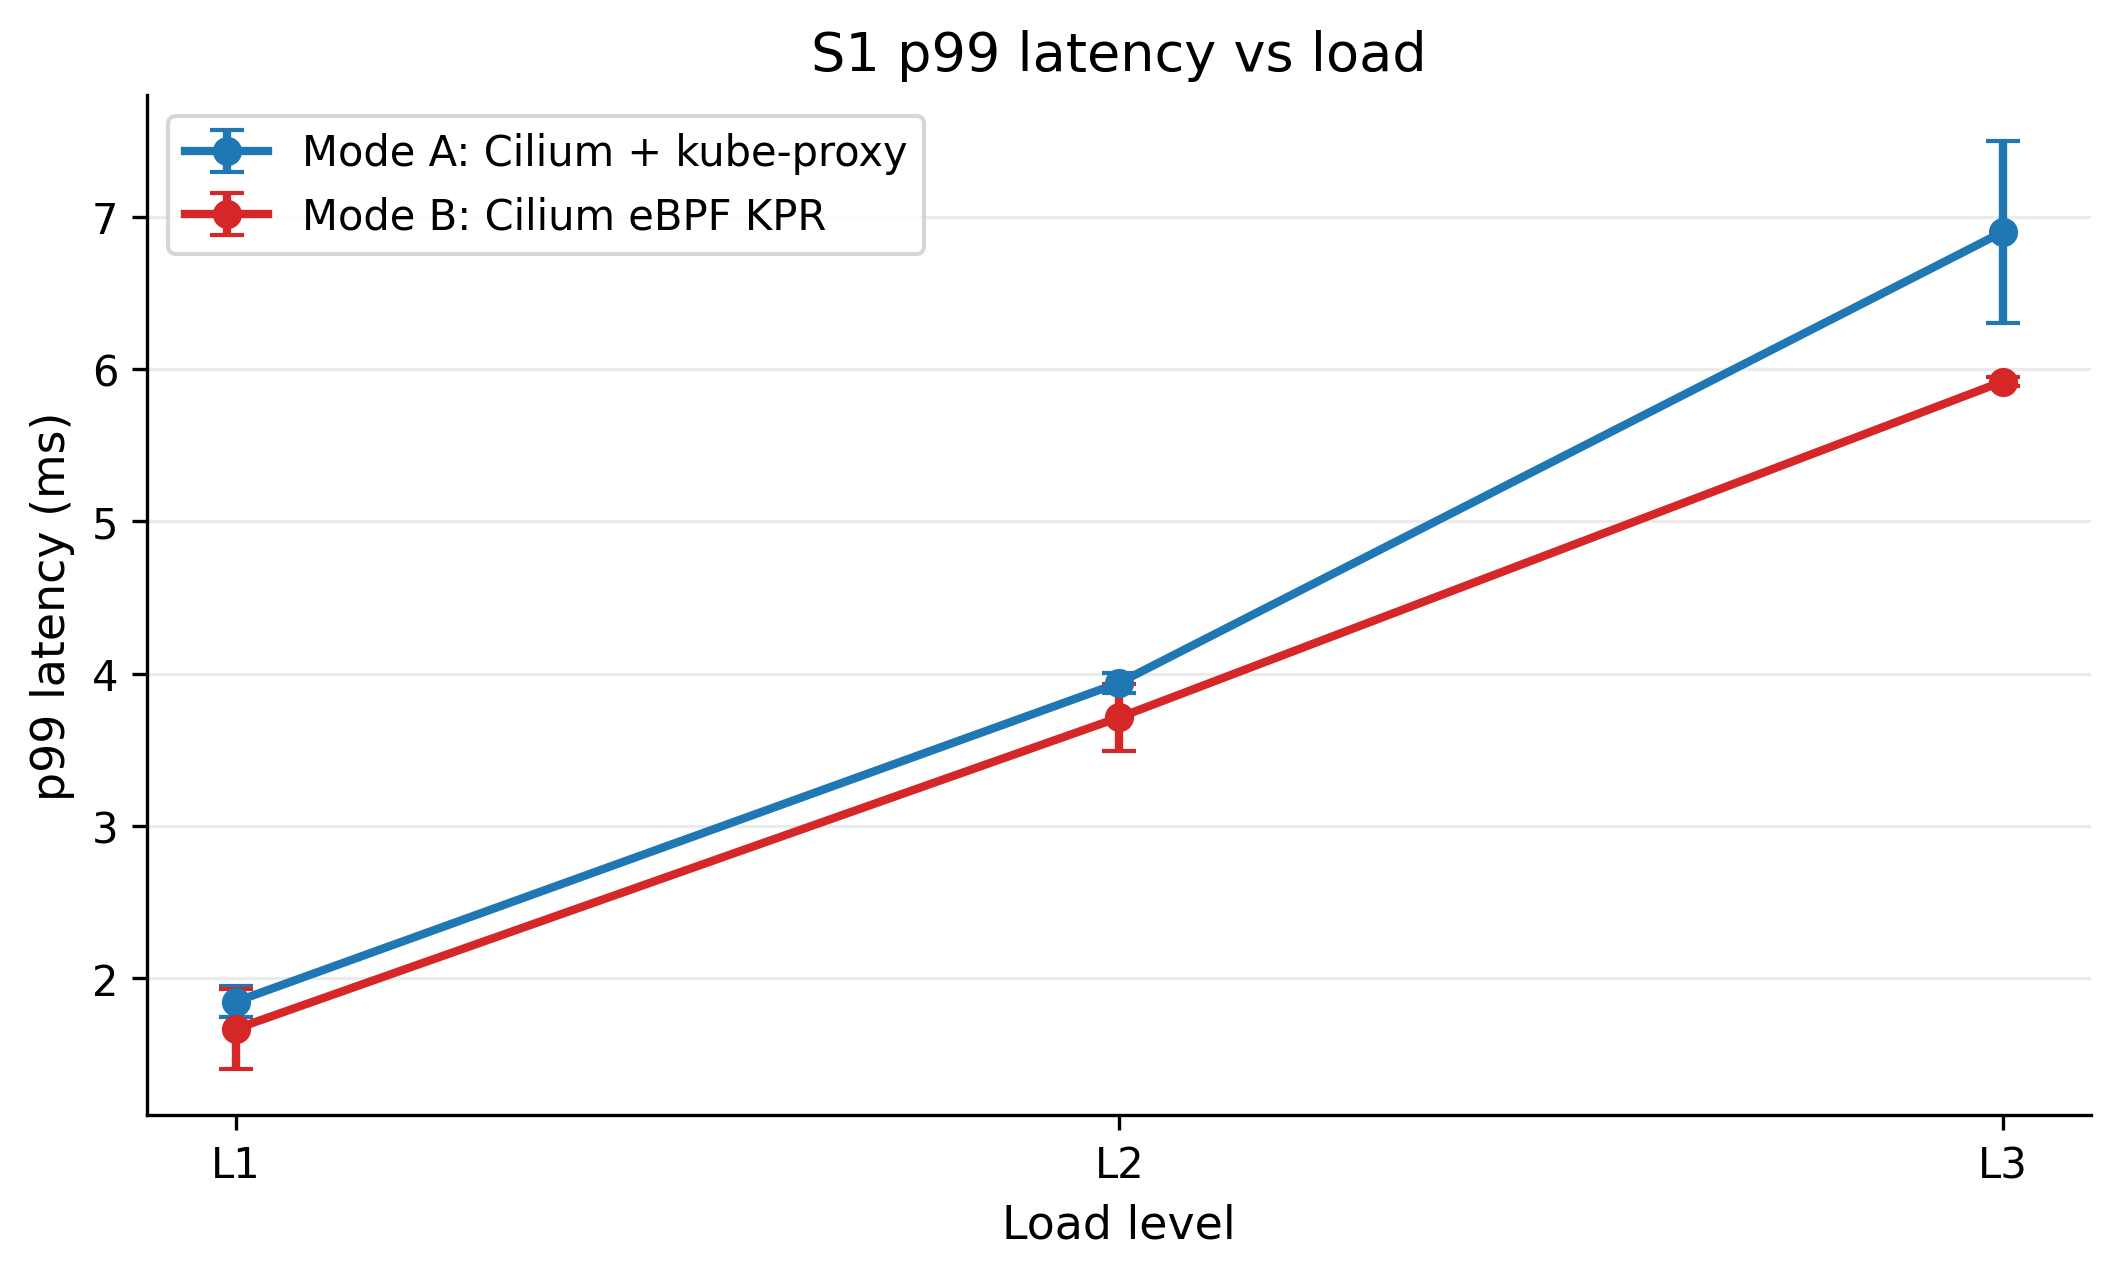
\includegraphics[width=0.90\textwidth]{../figures/thesis/fig-s1-p99-vs-load.png}
    \caption{P99 latency của S1 theo mức tải; các vạch dọc biểu diễn khoảng tin cậy 95\% quanh giá trị trung bình}
    \label{fig:s1-p99-vs-load}
\end{figure}

\begin{table}[H]
\centering
\caption{So sánh p99 latency trong S1}
\label{tab:s1-p99-summary}
\renewcommand{\arraystretch}{1.2}
\begin{tabularx}{\textwidth}{>{\raggedright\arraybackslash}p{1.2cm}>{\raggedleft\arraybackslash}p{2.0cm}>{\raggedleft\arraybackslash}p{2.0cm}>{\raggedleft\arraybackslash}p{2.0cm}>{\raggedleft\arraybackslash}p{1.5cm}>{\raggedright\arraybackslash}X}
\toprule
\textbf{Tải} & \textbf{Mode A p99} & \textbf{Mode B p99} & \textbf{Delta B/A} & \textbf{\(p\)} & \textbf{Diễn giải} \\
\midrule
L1 & 1.846 ms & 1.667 ms & -9.702\% & 0.0838 & Xu hướng, chưa significant \\
L2 & 3.939 ms & 3.712 ms & -5.766\% & 0.0377 & Significant \\
L3 & 6.899 ms & 5.917 ms & -14.223\% & 0.0191 & Significant \\
\bottomrule
\end{tabularx}
\end{table}

\textbf{Phân tích.} Hình~\ref{fig:s1-p99-vs-load} cho thấy p99 của cả hai mode tăng theo tải. Mode B có p99 trung bình thấp hơn Mode A ở cả ba mức tải. Tuy nhiên, L1 chỉ nên xem là xu hướng vì chưa significant. L2 và L3 có bằng chứng mạnh hơn; riêng L3 có delta lớn nhất, khoảng -14.2\%, nên cũng có ý nghĩa thực tế rõ hơn.

\begin{figure}[H]
    \centering
    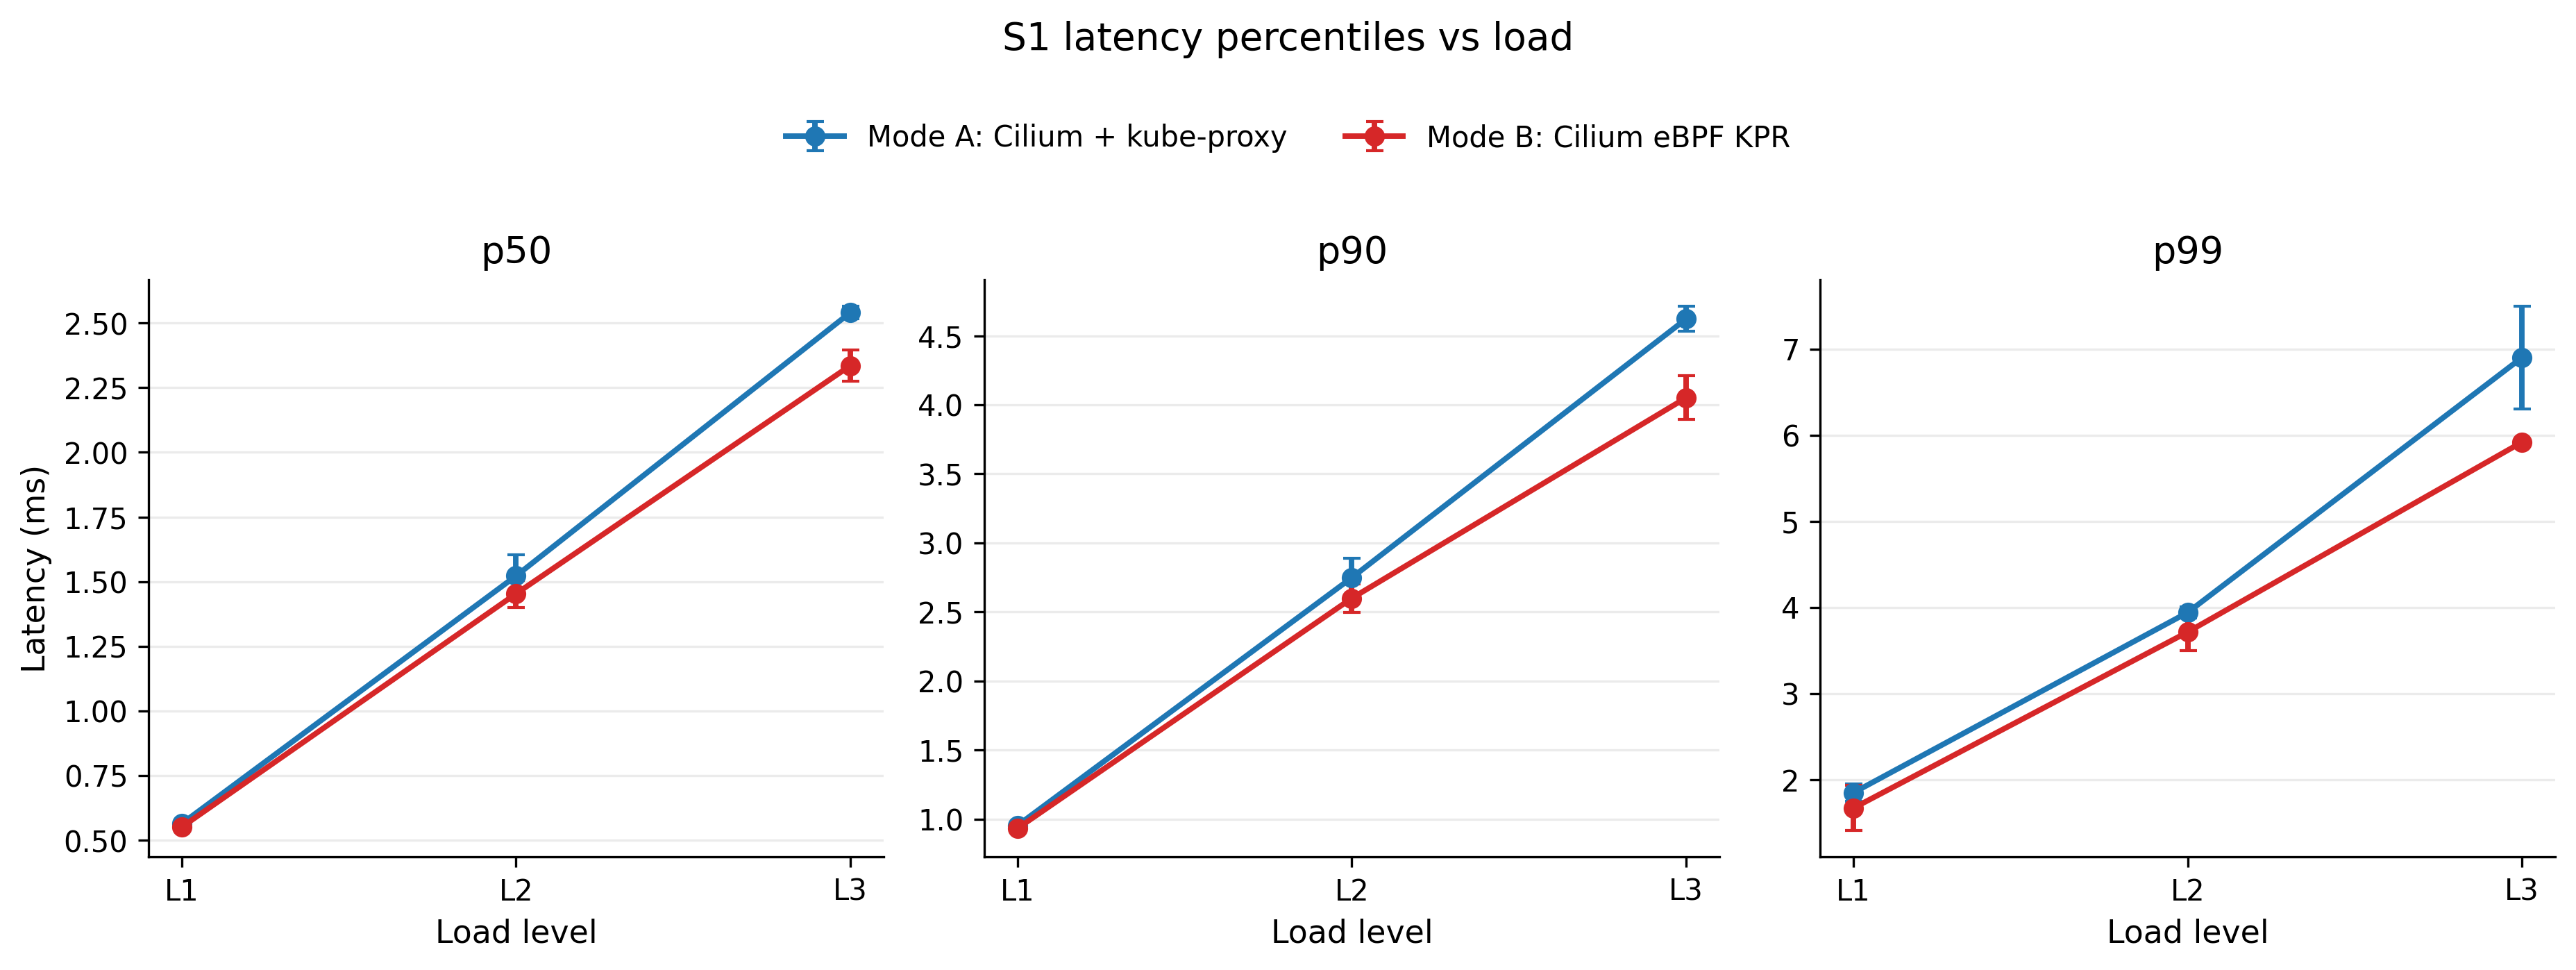
\includegraphics[width=0.90\textwidth]{../figures/thesis/fig-s1-latency-small-multiples.png}
    \caption{So sánh p50, p90 và p99 trong S1; các vạch dọc biểu diễn khoảng tin cậy 95\% quanh giá trị trung bình}
    \label{fig:s1-latency-small-multiples}
\end{figure}

Hình~\ref{fig:s1-latency-small-multiples} cho thấy ở L3, Mode B thấp hơn ở cả p50, p90 và p99. Vì xu hướng không chỉ xuất hiện ở một percentile đơn lẻ, kết quả S1 trở nên thuyết phục hơn.

\begin{figure}[H]
    \centering
    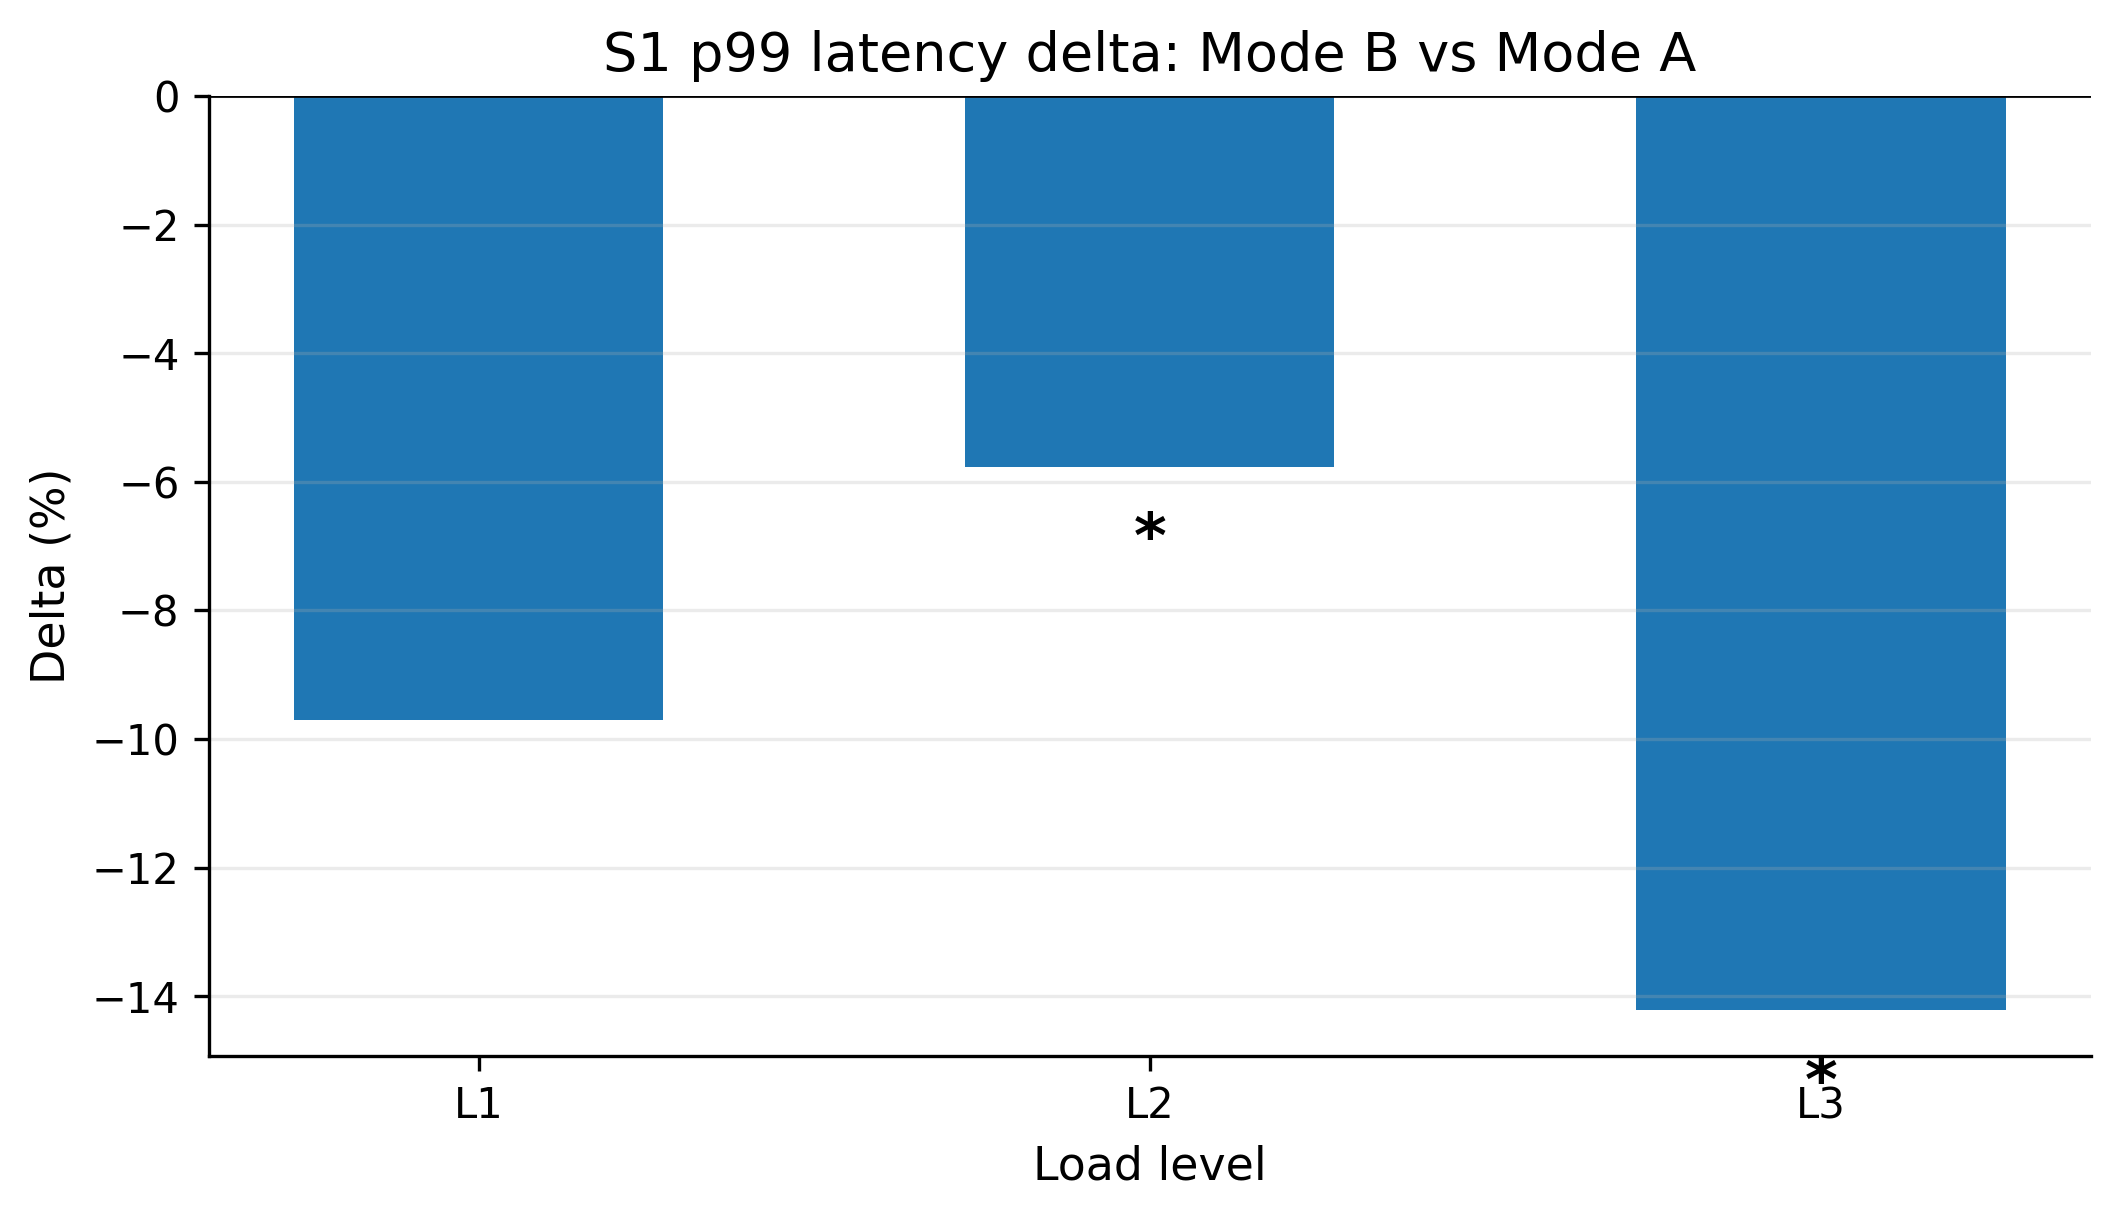
\includegraphics[width=0.82\textwidth]{../figures/thesis/fig-s1-delta-p99.png}
    \caption{Chênh lệch p99 của Mode B so với Mode A trong S1}
    \label{fig:s1-delta-p99}
\end{figure}

Hình~\ref{fig:s1-delta-p99} trình bày cùng kết quả dưới dạng delta phần trăm. Giá trị âm nghĩa là Mode B có p99 thấp hơn Mode A; điểm cần chú ý nhất là mức giảm tại L3.

Về cơ chế, S1 phù hợp để liên hệ kết quả với service datapath. Mode A dựa trên kube-proxy/iptables, DNAT và conntrack; Mode B dùng Cilium eBPF kube-proxy replacement. Khi tải tăng, chi phí nhỏ trên từng request dễ tích lũy ở phần đuôi, làm khác biệt p99 rõ hơn.

Hình~\ref{fig:s1-grafana-cpu-evidence} và Hình~\ref{fig:s1-grafana-memory-evidence} là bằng chứng vận hành hỗ trợ cho S1 L3. Hai hình dùng panel namespace-level để kiểm tra CPU và memory của namespace benchmark; các ảnh S1 L2 và bản phóng lớn được đặt ở Phụ lục~E.

Các ảnh không cho thấy dấu hiệu CPU hoặc memory pressure nghiêm trọng trong cửa sổ S1 L3. Vì đây chỉ là screenshot telemetry, chúng được dùng như sanity check, không phải bằng chứng định lượng để giải thích trực tiếp chênh lệch p99.

\begin{figure}[H]
    \centering
    \textbf{Mode A -- CPU namespace}\\[0.25em]
    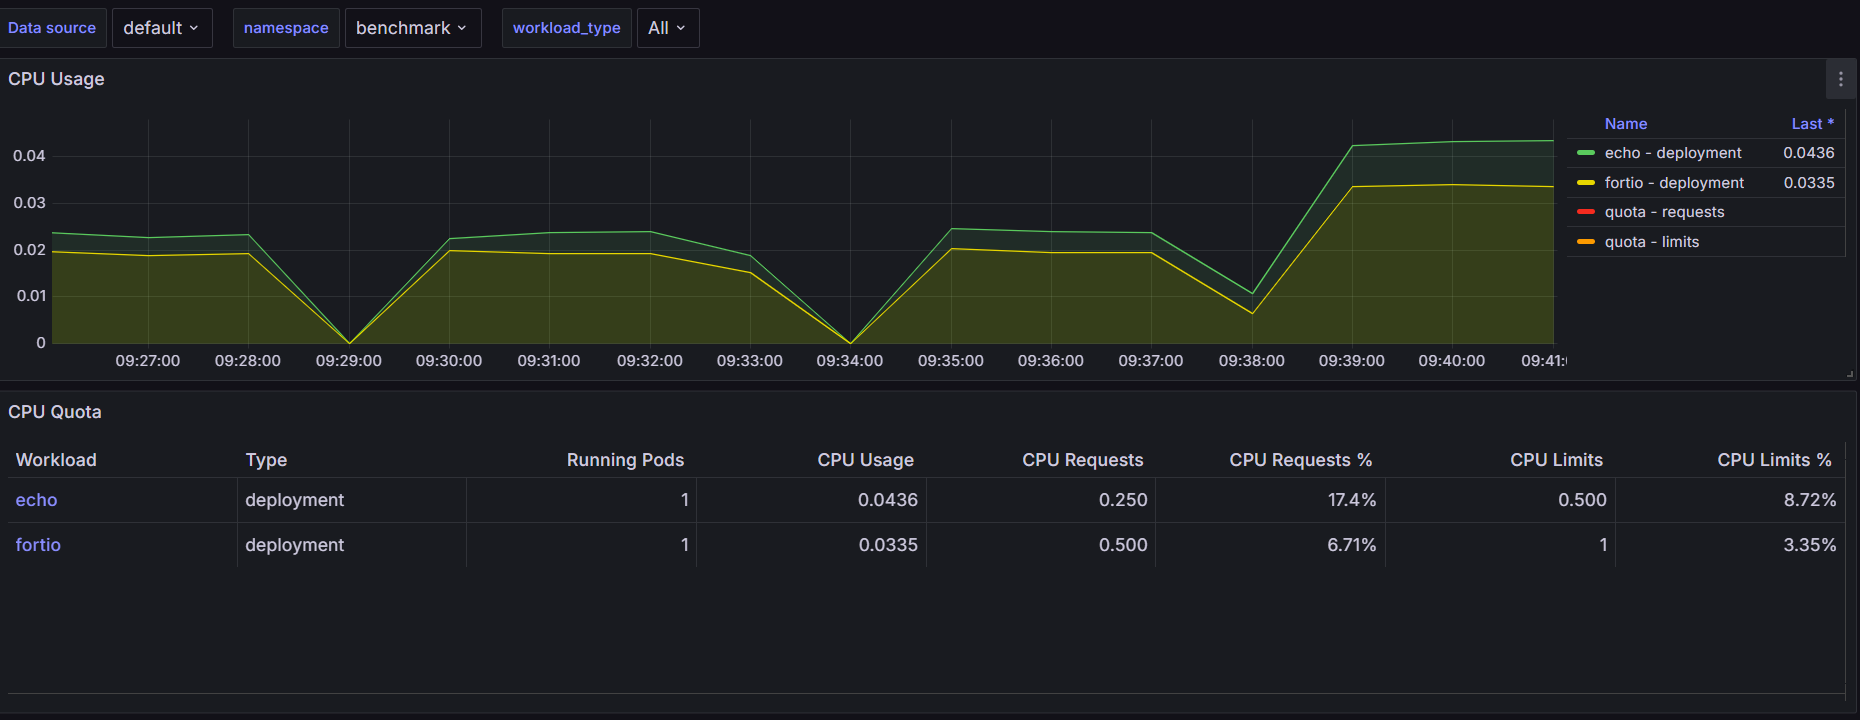
\includegraphics[width=0.88\textwidth]{../figures/grafana/modeA/grafana-ns-cpu-S1-L3-R1.png}
    \vspace{0.5em}
    
    \textbf{Mode B -- CPU namespace}\\[0.25em]
    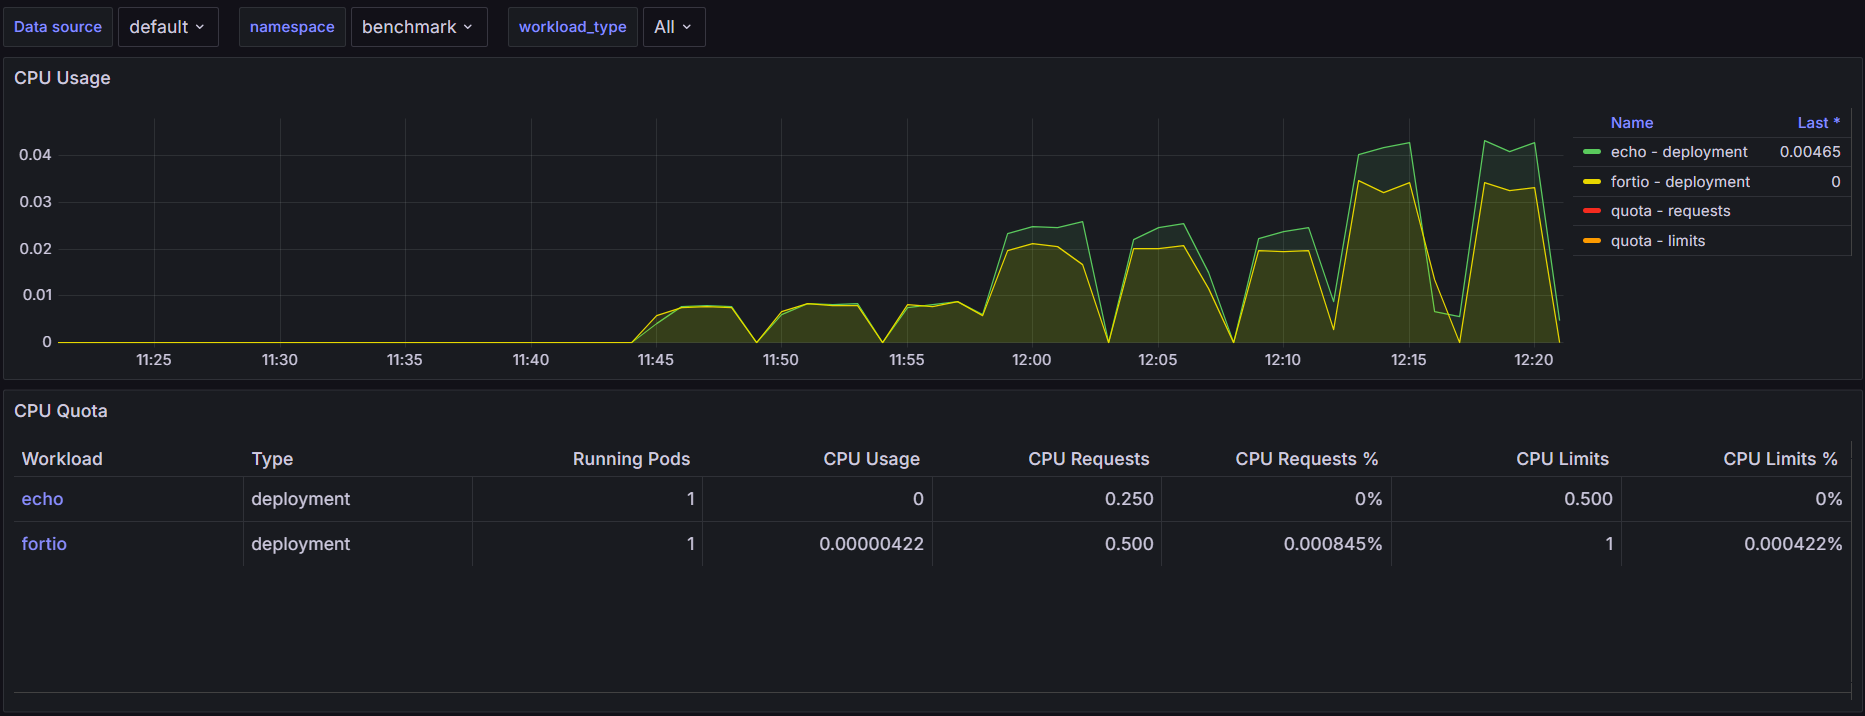
\includegraphics[width=0.88\textwidth]{../figures/grafana/modeB/grafana-ns-cpu-S1-L3.png}
    \caption{Bằng chứng Grafana namespace-level về CPU cho S1 L3 ở Mode A và Mode B; ảnh dùng để kiểm tra bối cảnh vận hành và không phải kết quả hiệu năng chính}
    \label{fig:s1-grafana-cpu-evidence}
\end{figure}

\begin{figure}[H]
    \centering
    \textbf{Mode A -- memory namespace}\\[0.25em]
    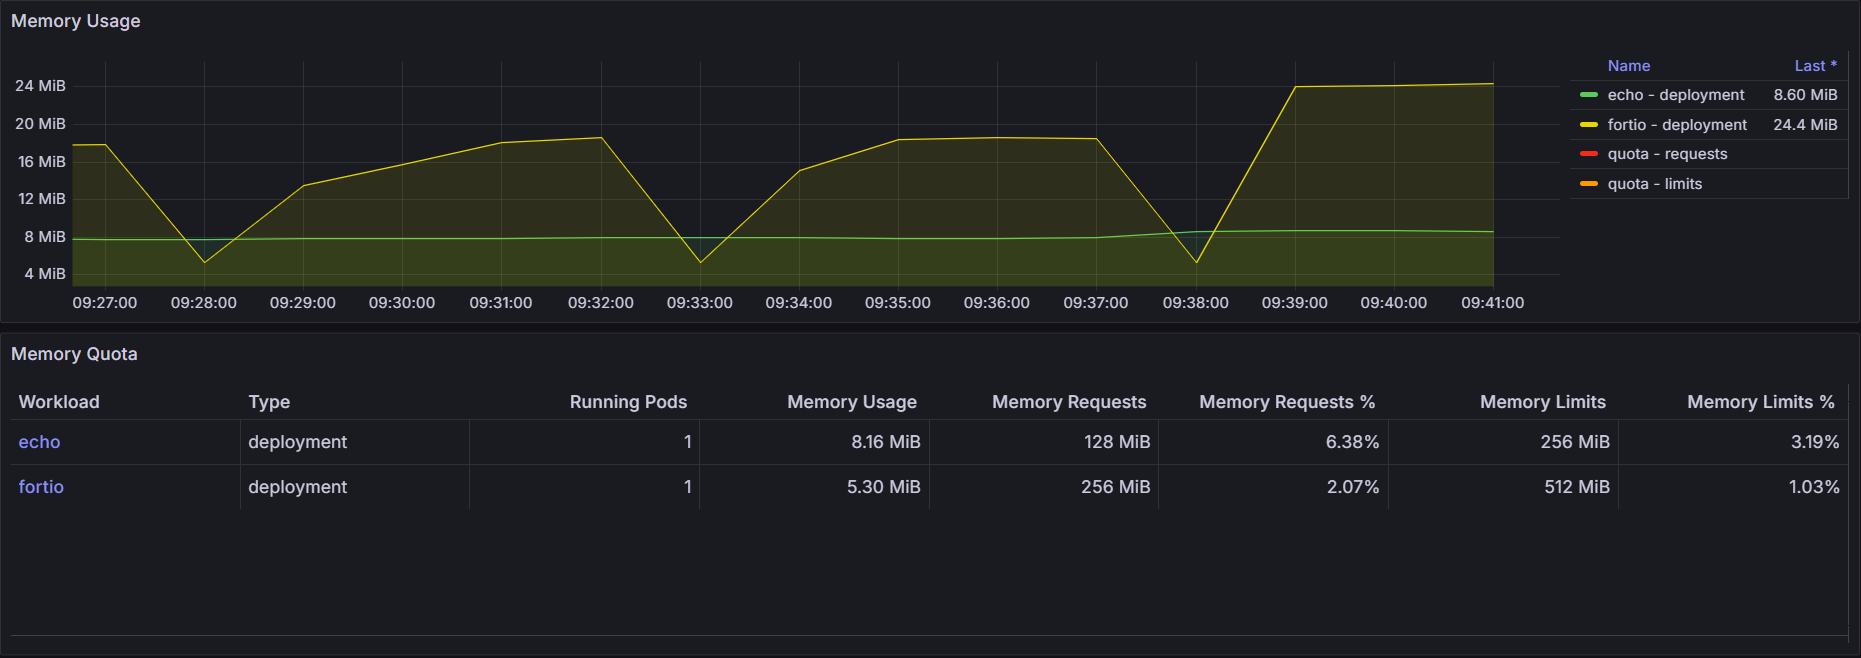
\includegraphics[width=0.88\textwidth]{../figures/grafana/modeA/grafana-ns-mem-S1-L3-R1.png}
    \vspace{0.5em}

    \textbf{Mode B -- memory namespace}\\[0.25em]
    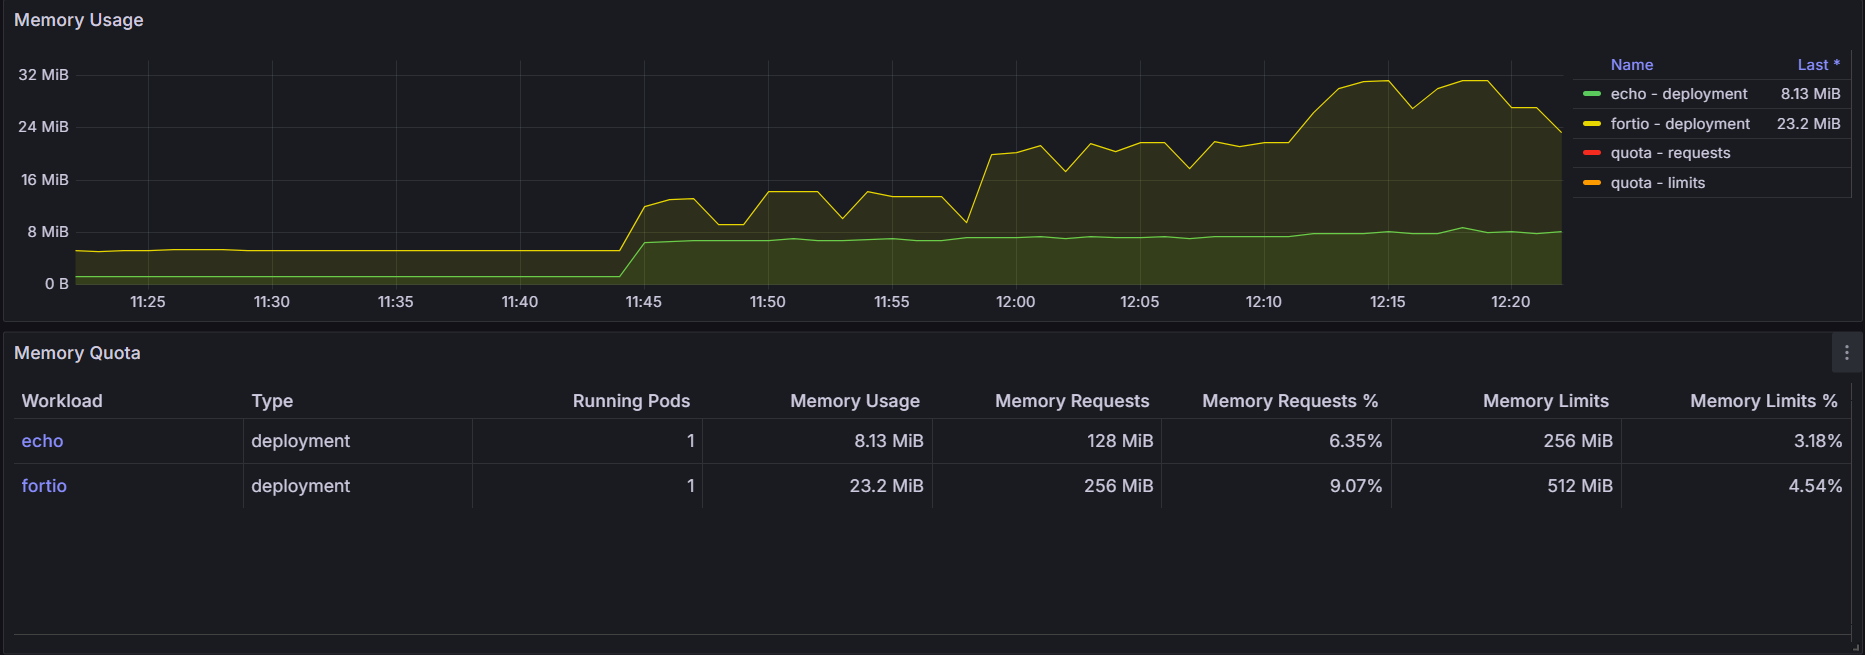
\includegraphics[width=0.88\textwidth]{../figures/grafana/modeB/grafana-ns-mem-S1-L3.png}
    \caption{Bằng chứng Grafana namespace-level về memory cho S1 L3 ở Mode A và Mode B; ảnh dùng để kiểm tra bối cảnh vận hành và không phải kết quả hiệu năng chính}
    \label{fig:s1-grafana-memory-evidence}
\end{figure}

\textbf{Kết luận.} Trong S1, Mode B cho thấy lợi thế p99 rõ hơn ở L2 và L3; L1 chỉ nên viết như xu hướng. Kết quả phù hợp với kỳ vọng về eBPF service datapath, nhưng không chứng minh Mode B luôn nhanh hơn trong mọi cluster hoặc workload.

\section{Kết quả S2: stress và thay đổi kết nối}

S2 kiểm tra hai mode dưới workload có nhiều pha, burst và connection churn. Kết quả không nên gộp thành một giá trị trung bình duy nhất, vì ramp-up, sustained, burst và cooldown tạo các trạng thái tải khác nhau. Cấu trúc này làm p99 nhạy hơn với trạng thái kết nối, cache, scheduling và dao động hệ thống.

Pipeline vẫn tổng hợp p50 và p90 cho S2, nhưng phần thân chương ưu tiên p99 vì mục tiêu chính là tail latency dưới burst và connection churn. Hai biểu đồ p99 theo pha là nguồn phân tích chính. Heatmap chỉ đóng vai trò tóm tắt hướng chênh lệch theo load và phase.

\subsection{S2 tại L2}

Hình~\ref{fig:s2-phase-p99-l2} cho thấy S2 tại L2 có kết quả pha trộn. Mode B thấp hơn Mode A ở phần lớn pha, nhưng không nhất quán trong toàn bộ run.

\begin{figure}[H]
    \centering
    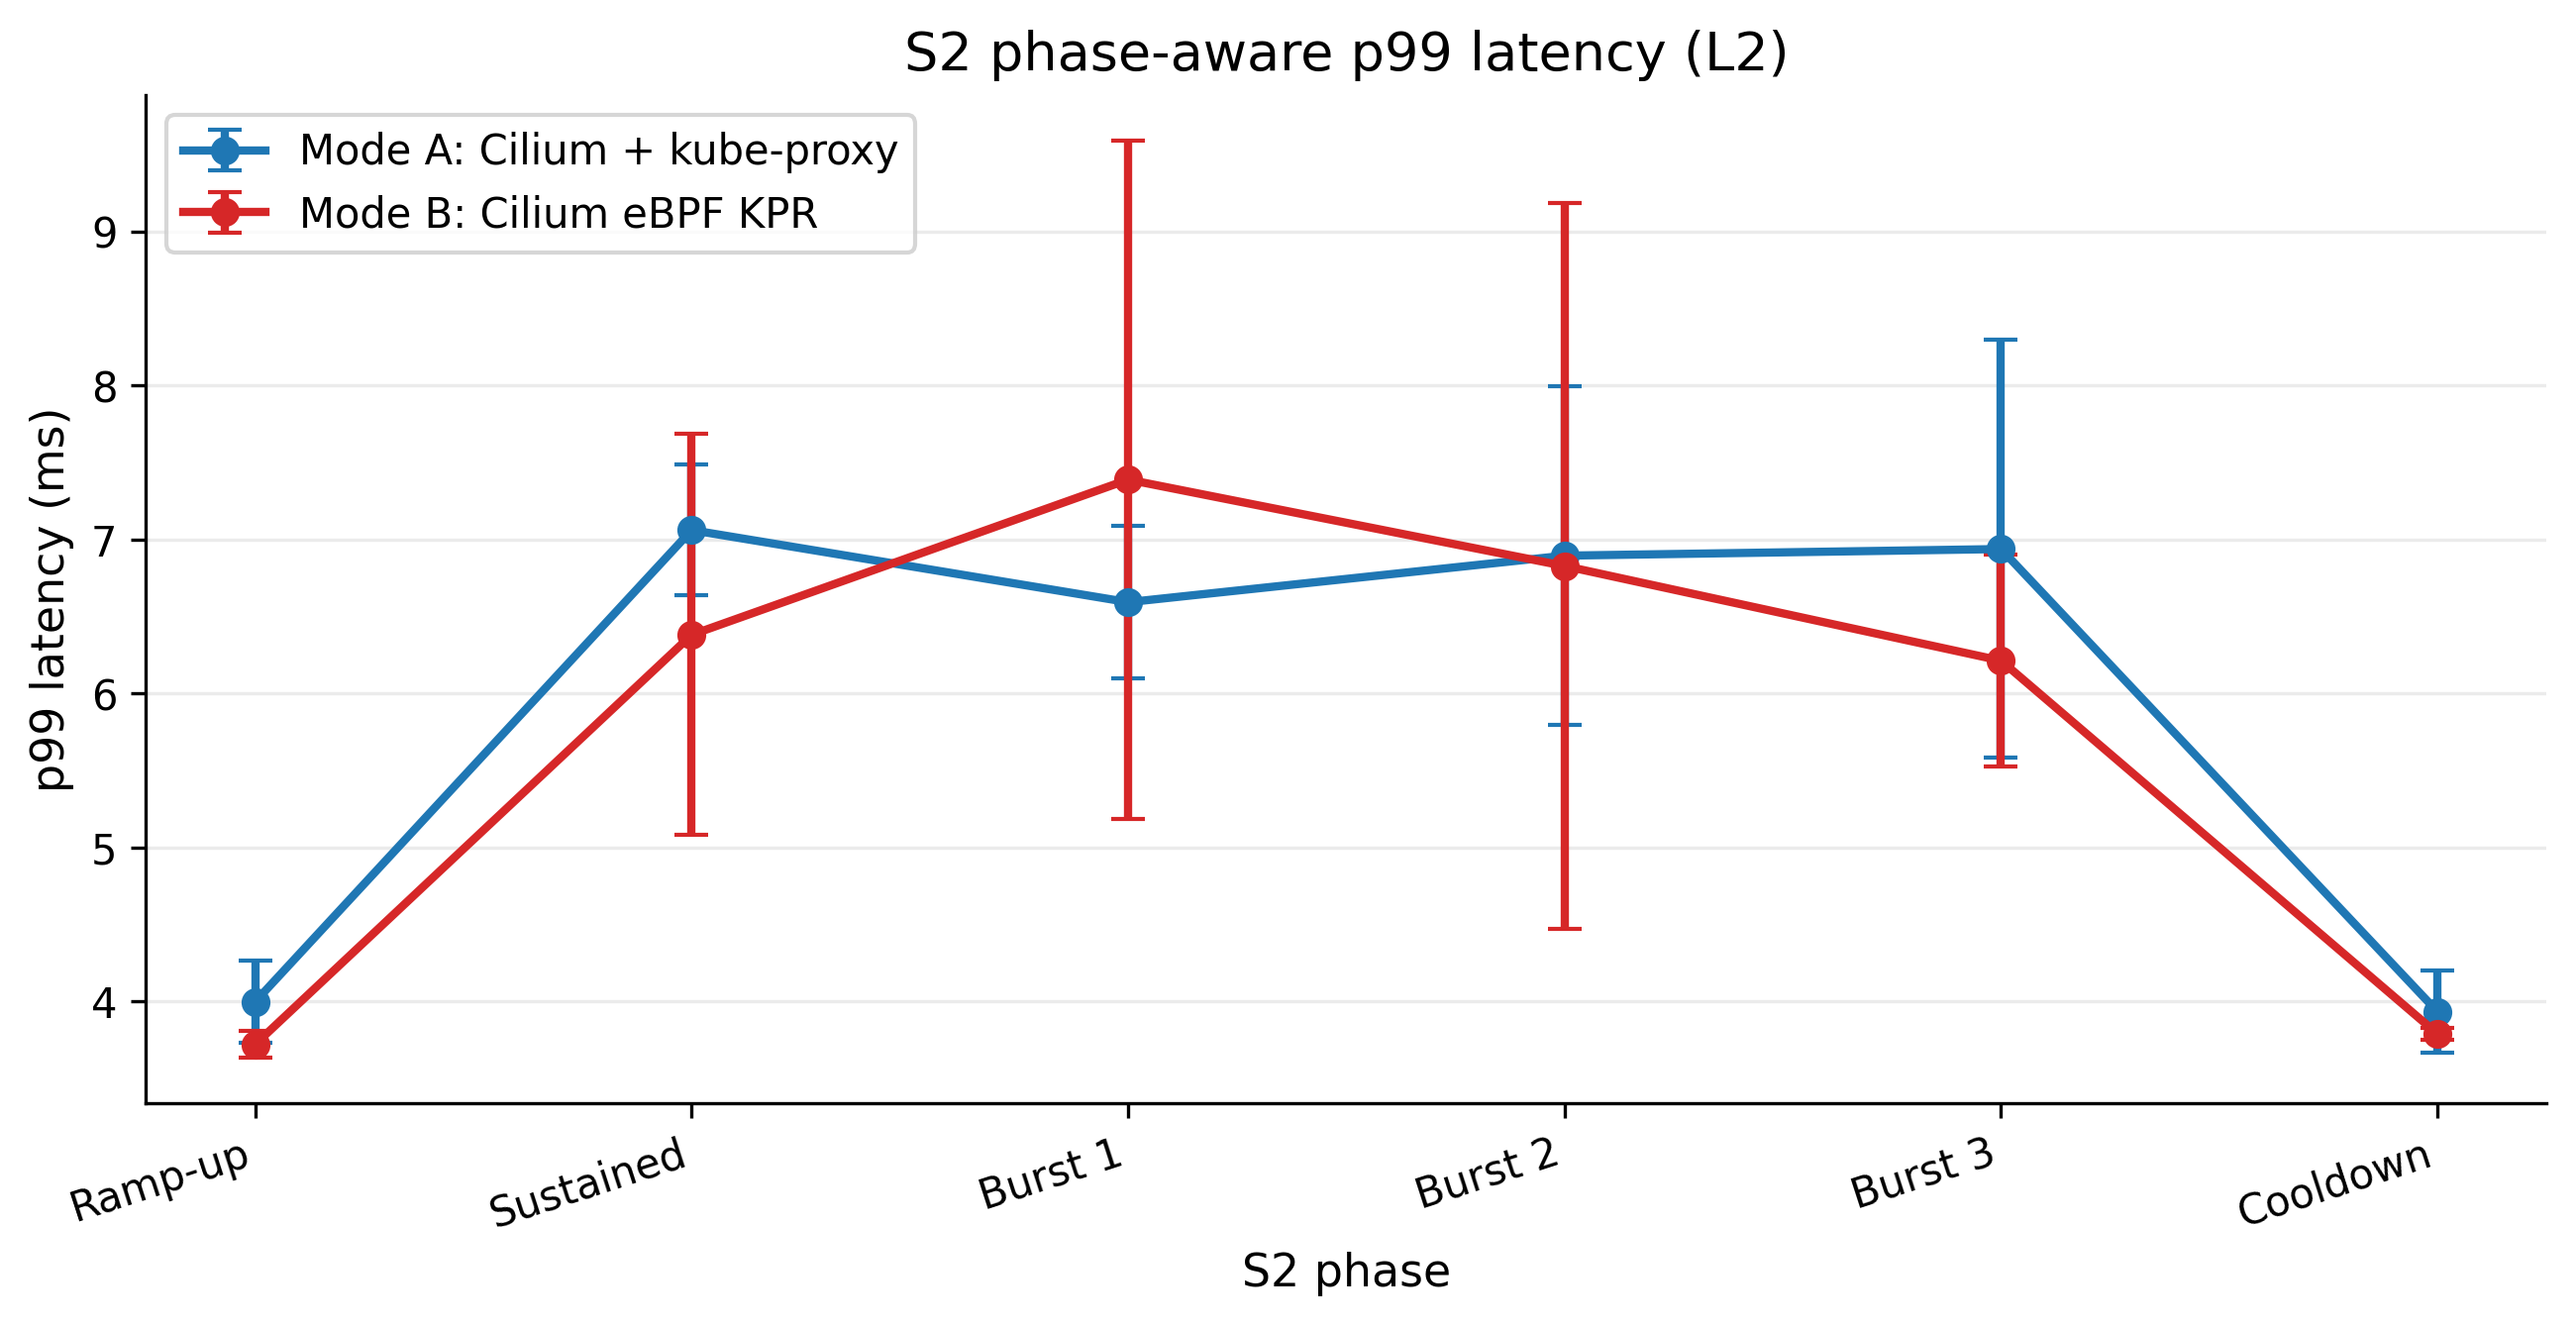
\includegraphics[width=0.90\textwidth]{../figures/thesis/fig-s2-phase-p99-l2.png}
    \caption{P99 latency theo pha trong S2 L2; các vạch dọc biểu diễn khoảng tin cậy 95\% quanh giá trị trung bình}
    \label{fig:s2-phase-p99-l2}
\end{figure}

\begin{table}[H]
\centering
\caption{So sánh p99 theo pha trong S2 L2}
\label{tab:s2-l2-p99-summary}
\small
\setlength{\tabcolsep}{4pt}
\renewcommand{\arraystretch}{1.2}
\begin{tabularx}{\textwidth}{>{\raggedright\arraybackslash}p{2.35cm}>{\raggedleft\arraybackslash}p{1.55cm}>{\raggedleft\arraybackslash}p{1.55cm}>{\raggedleft\arraybackslash}p{1.55cm}>{\raggedleft\arraybackslash}p{1.1cm}>{\raggedright\arraybackslash}X}
\toprule
\textbf{Pha} & \textbf{Mode A} & \textbf{Mode B} & \textbf{Delta} & \textbf{\(p\)} & \textbf{Diễn giải} \\
\midrule
Ramp-up & 3.998 ms & 3.721 ms & -6.934\% & 0.0367 & Significant \\
Sustained & 7.061 ms & 6.381 ms & -9.628\% & 0.1438 & Xu hướng \\
Burst 1 & 6.593 ms & 7.389 ms & +12.081\% & 0.2571 & Ngoại lệ, không significant \\
Burst 2 & 6.895 ms & 6.828 ms & -0.972\% & 0.9191 & Gần tương đương \\
Burst 3 & 6.938 ms & 6.213 ms & -10.445\% & 0.1339 & Xu hướng \\
Cooldown & 3.933 ms & 3.789 ms & -3.668\% & 0.1423 & Xu hướng nhẹ \\
\bottomrule
\end{tabularx}
\end{table}

\textbf{Phân tích.} Ở ramp-up, Mode B thấp hơn Mode A khoảng 6.9\% và đây là pha p99 duy nhất tại S2 L2 được đánh dấu significant. Sustained và Burst 3 cũng nghiêng về Mode B, nhưng chỉ nên xem là xu hướng. Ngoại lệ chính là Burst 1: Mode B cao hơn Mode A khoảng 12.1\%, dù chênh lệch này không significant. Burst 2 gần như tương đương.

Burst 1 là đợt tăng tải đột ngột đầu tiên sau sustained. Trong cửa sổ ngắn như vậy, một vài request chậm có thể kéo p99 lên rõ. Giá trị \(p=0.2571\) cho thấy chênh lệch này chưa đủ mạnh về mặt thống kê. Vì vậy, S2 L2 nên được đọc như vùng chuyển tiếp: Mode B tốt hơn ở một số pha, nhưng kết quả chưa đồng đều.

\textbf{Kết luận.} Với S2 L2, kết quả có lợi cho Mode B ở một số pha nhưng chưa đủ đồng đều để kết luận mạnh. Burst 1 là lời nhắc quan trọng rằng workload động cần được đọc theo phase, không nên gộp thành một nhận xét chung.

\subsection{S2 tại L3}

Hình~\ref{fig:s2-phase-p99-l3} trình bày S2 tại L3. Ở mức tải cao hơn, sustained và burst làm tail latency nhạy hơn. Khác với L2, Mode B có p99 trung bình thấp hơn Mode A ở tất cả các pha.

\begin{figure}[H]
    \centering
    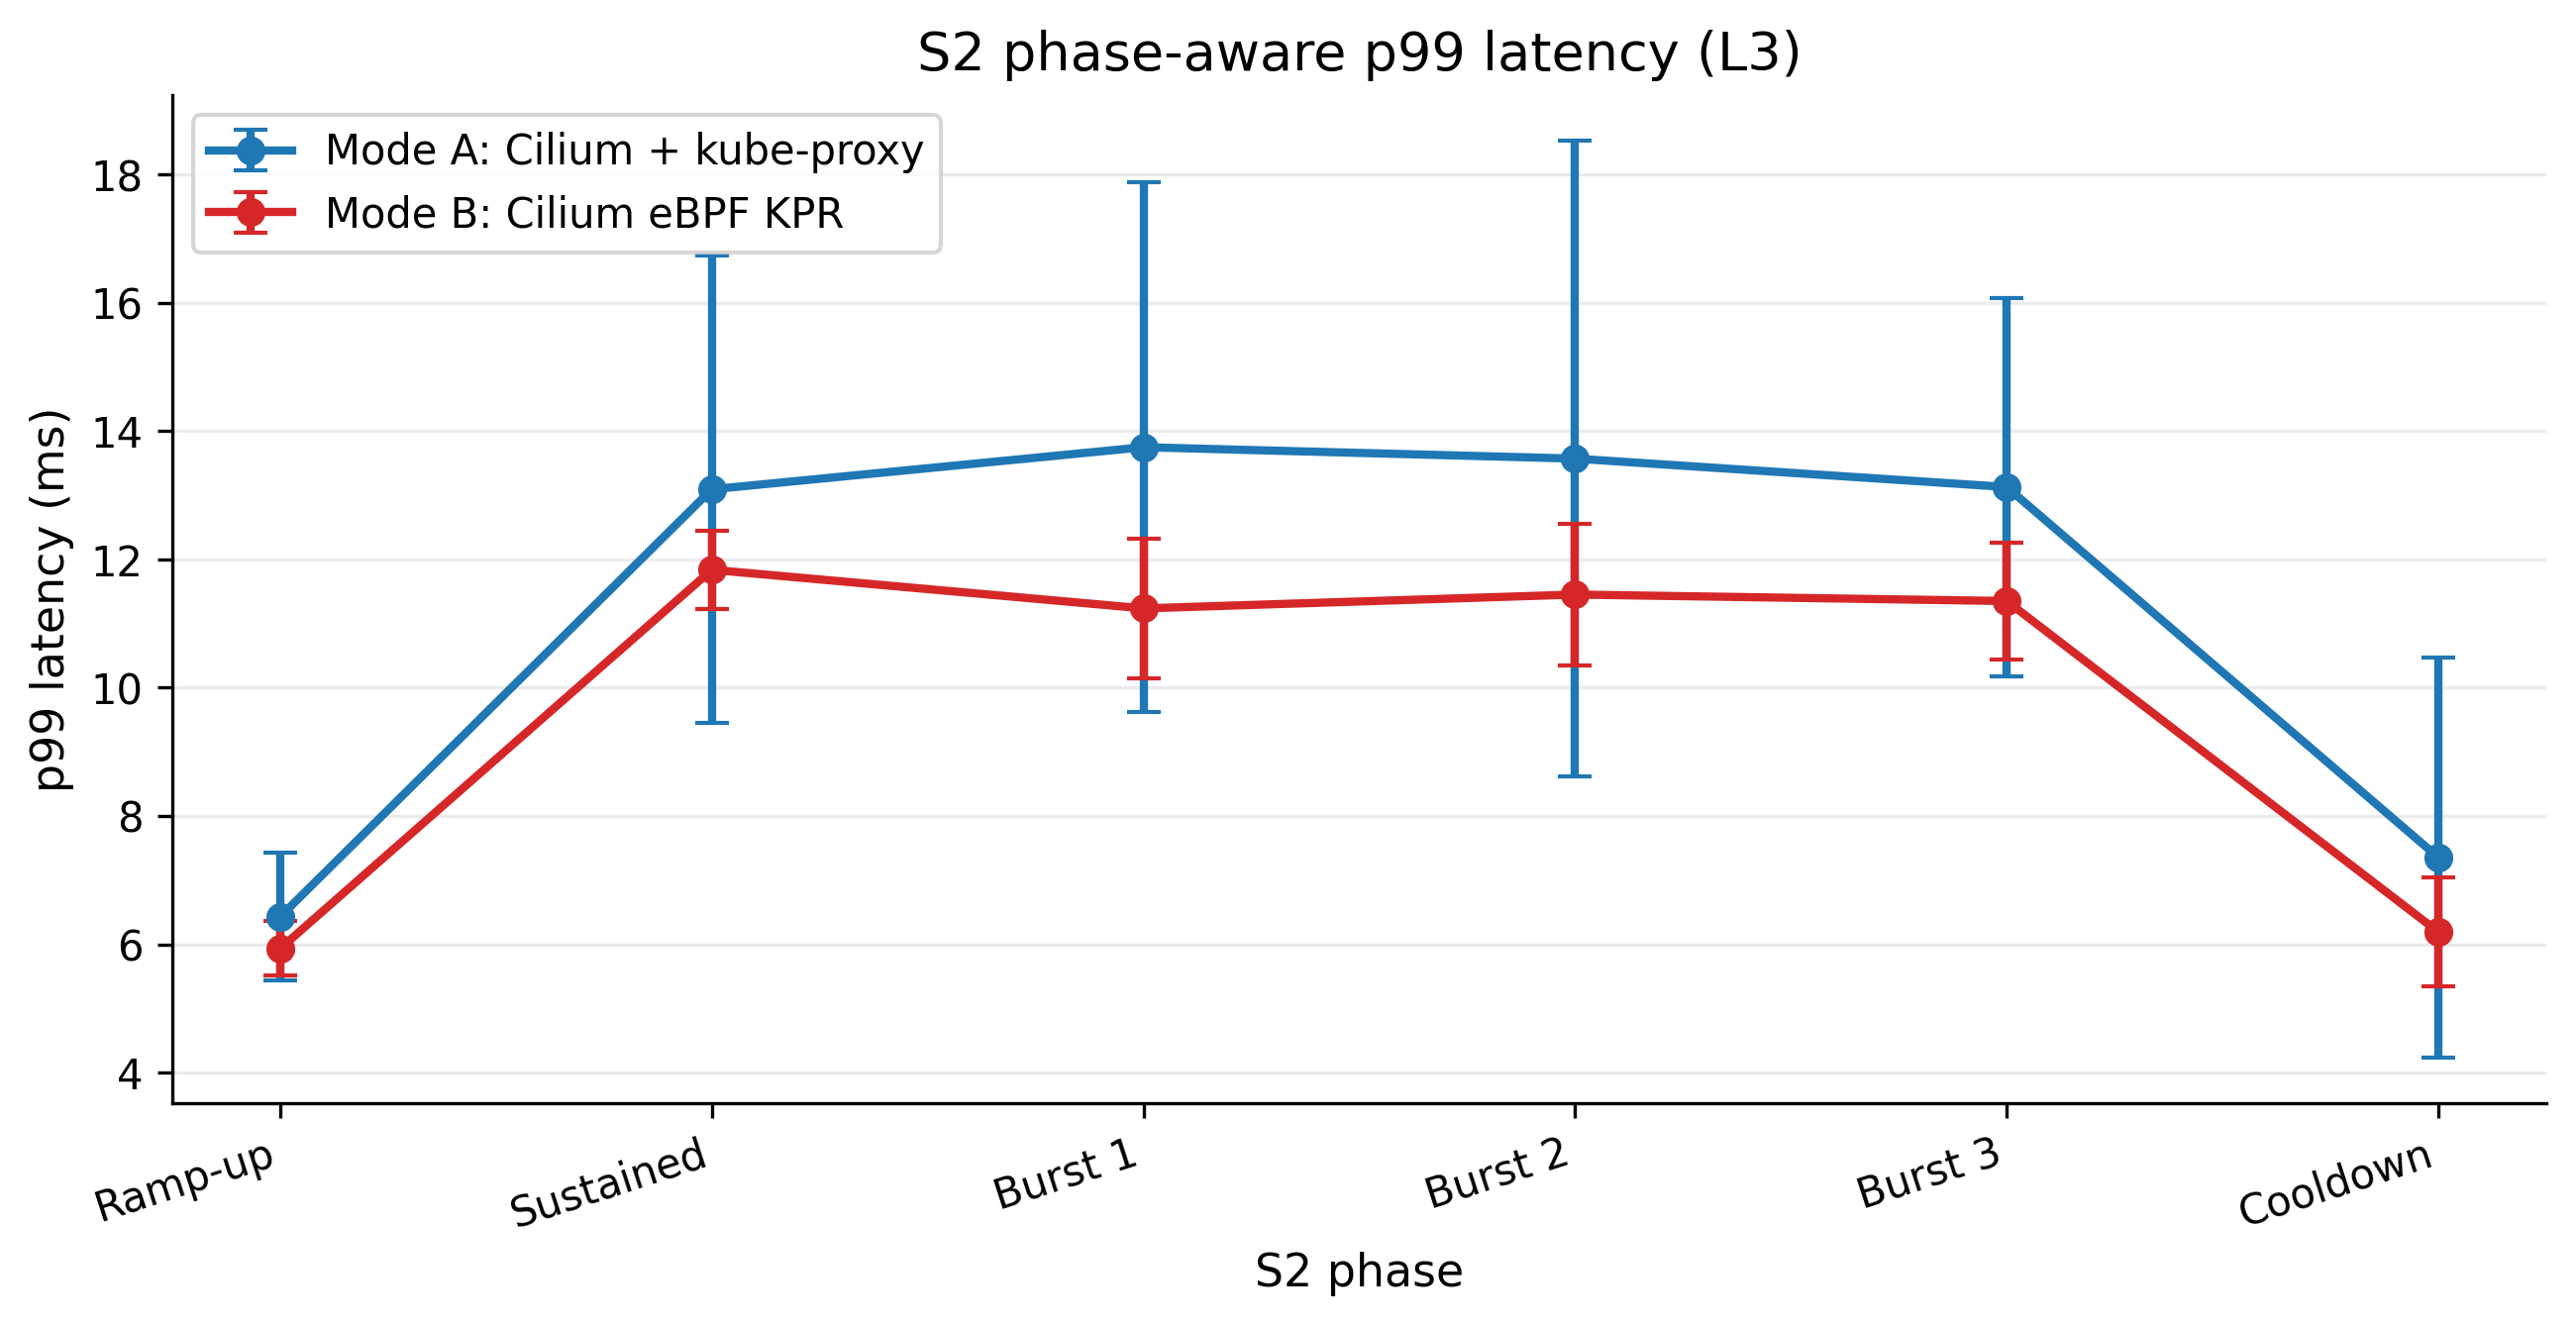
\includegraphics[width=0.90\textwidth]{../figures/thesis/fig-s2-phase-p99-l3.png}
    \caption{P99 latency theo pha trong S2 L3; các vạch dọc biểu diễn khoảng tin cậy 95\% quanh giá trị trung bình}
    \label{fig:s2-phase-p99-l3}
\end{figure}

\begin{table}[H]
\centering
\caption{So sánh p99 theo pha trong S2 L3}
\label{tab:s2-l3-p99-summary}
\small
\setlength{\tabcolsep}{4pt}
\renewcommand{\arraystretch}{1.2}
\begin{tabularx}{\textwidth}{>{\raggedright\arraybackslash}p{2.35cm}>{\raggedleft\arraybackslash}p{1.55cm}>{\raggedleft\arraybackslash}p{1.55cm}>{\raggedleft\arraybackslash}p{1.55cm}>{\raggedleft\arraybackslash}p{1.1cm}>{\raggedright\arraybackslash}X}
\toprule
\textbf{Pha} & \textbf{Mode A} & \textbf{Mode B} & \textbf{Delta} & \textbf{\(p\)} & \textbf{Diễn giải} \\
\midrule
Ramp-up & 6.431 ms & 5.934 ms & -7.724\% & 0.1531 & Xu hướng \\
Sustained & 13.094 ms & 11.839 ms & -9.587\% & 0.2751 & Xu hướng \\
Burst 1 & 13.750 ms & 11.237 ms & -18.271\% & 0.1119 & Xu hướng mạnh \\
Burst 2 & 13.572 ms & 11.453 ms & -15.618\% & 0.2029 & Xu hướng mạnh \\
Burst 3 & 13.129 ms & 11.352 ms & -13.532\% & 0.1116 & Xu hướng \\
Cooldown & 7.355 ms & 6.193 ms & -15.800\% & 0.2466 & Xu hướng \\
\bottomrule
\end{tabularx}
\end{table}

\textbf{Phân tích.} Ở L3, toàn bộ delta p99 đều âm. Các pha burst có chênh lệch lớn hơn: Burst 1 khoảng -18.3\%, Burst 2 khoảng -15.6\% và Burst 3 khoảng -13.5\%. Đây là mức chênh đáng chú ý vì xuất hiện ở tải cao, đúng nơi tail latency dễ bộc lộ nhất.

Điểm cần thận trọng là các dòng p99 L3 chưa significant. Vạch CI của Mode A dài hơn Mode B ở nhiều pha, đặc biệt sustained và burst, cho thấy p99 của Mode A dao động nhiều hơn giữa ba lần chạy. Vì các \(p\)-value vẫn lớn hơn 0.05, kết luận phù hợp là Mode B có xu hướng p99 thấp hơn và ổn định hơn trong tập run hiện tại, nhưng chưa đủ để khẳng định chắc chắn cho từng pha.

Về cơ chế, L3 đặt datapath vào vùng nhạy với tail latency hơn. Khi tải nền cao và burst xuất hiện, queueing, trạng thái kết nối và scheduling jitter dễ tích lũy vào p99. Mẫu hình toàn delta âm phù hợp với giả thuyết Mode B có lợi thế ở tải cao, nhưng vẫn chịu giới hạn bởi variance và số lần lặp nhỏ.

\textbf{Kết luận.} S2 L3 là phần ủng hộ rõ nhất cho nhận định rằng Mode B có thể có lợi thế tail latency trong workload động ở tải cao. Dù vậy, vì chưa significant ở từng pha, cách viết phù hợp là ``xu hướng mạnh'' thay vì khẳng định tuyệt đối.

\subsection{Vai trò của heatmap S2}

Hình~\ref{fig:s2-p99-delta-heatmap} tóm tắt chênh lệch p99 của Mode B so với Mode A theo pha và mức tải. Giá trị âm nghĩa là Mode B thấp hơn; giá trị dương nghĩa là Mode B cao hơn.

\begin{figure}[H]
    \centering
    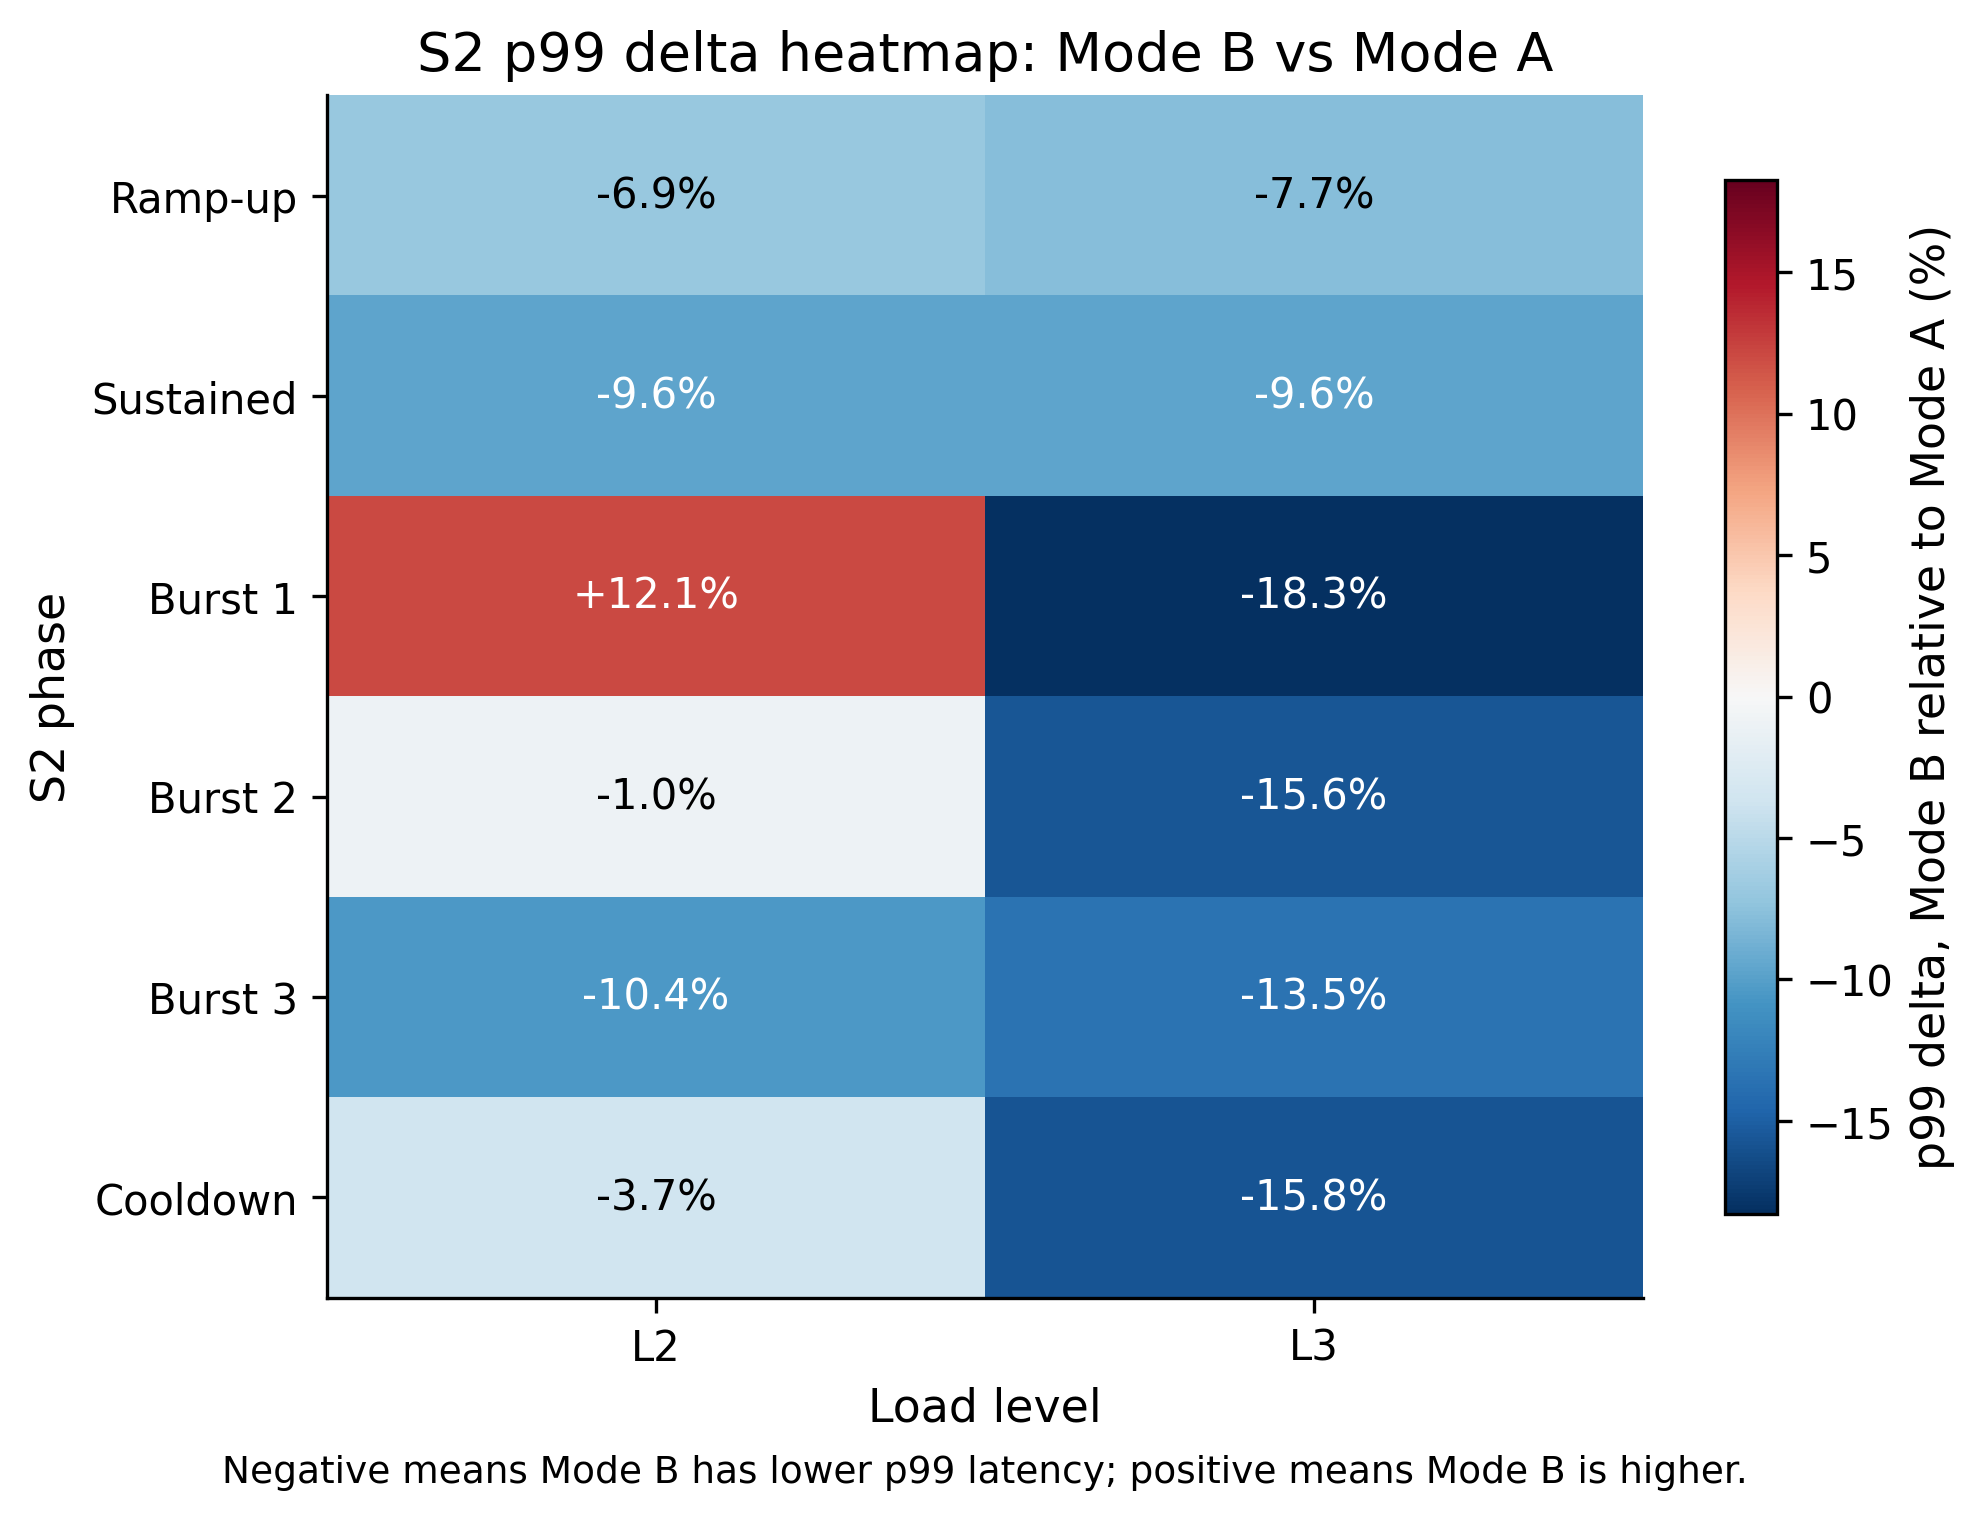
\includegraphics[width=0.78\textwidth]{../figures/thesis/fig-s2-p99-delta-heatmap.png}
    \caption{Heatmap chênh lệch p99 trong S2 theo pha và mức tải}
    \label{fig:s2-p99-delta-heatmap}
\end{figure}

\textbf{Phân tích.} Heatmap cho thấy hai điểm chính: L3 có delta âm ở toàn bộ pha, còn L2 có ngoại lệ Burst 1 dương. Hình này giúp nhận diện nhanh mẫu hình theo pha, nhưng chỉ thể hiện chênh lệch trung bình. Vì vậy, diễn giải chính vẫn phải dựa vào biểu đồ p99 theo pha, CI, \(p\)-value và độ biến động.

Hình~\ref{fig:s2-grafana-cpu-evidence} và Hình~\ref{fig:s2-grafana-memory-evidence} bổ sung bối cảnh vận hành cho S2 L3. Hai hình kiểm tra CPU và memory của namespace benchmark ở mức tải stress cao hơn.

Trong cửa sổ S2 L3 được lưu, không thấy dấu hiệu CPU hoặc memory pressure nghiêm trọng. Tuy nhiên, ảnh Grafana không được căn chỉnh chính xác theo từng pha, nên chỉ dùng như sanity check, không dùng để quy kết spike p99 cho CPU/memory. Các ảnh S2 L2 và bản phóng lớn được đặt ở Phụ lục~E.

\begin{figure}[H]
    \centering
    \textbf{Mode A -- CPU namespace}\\[0.25em]
    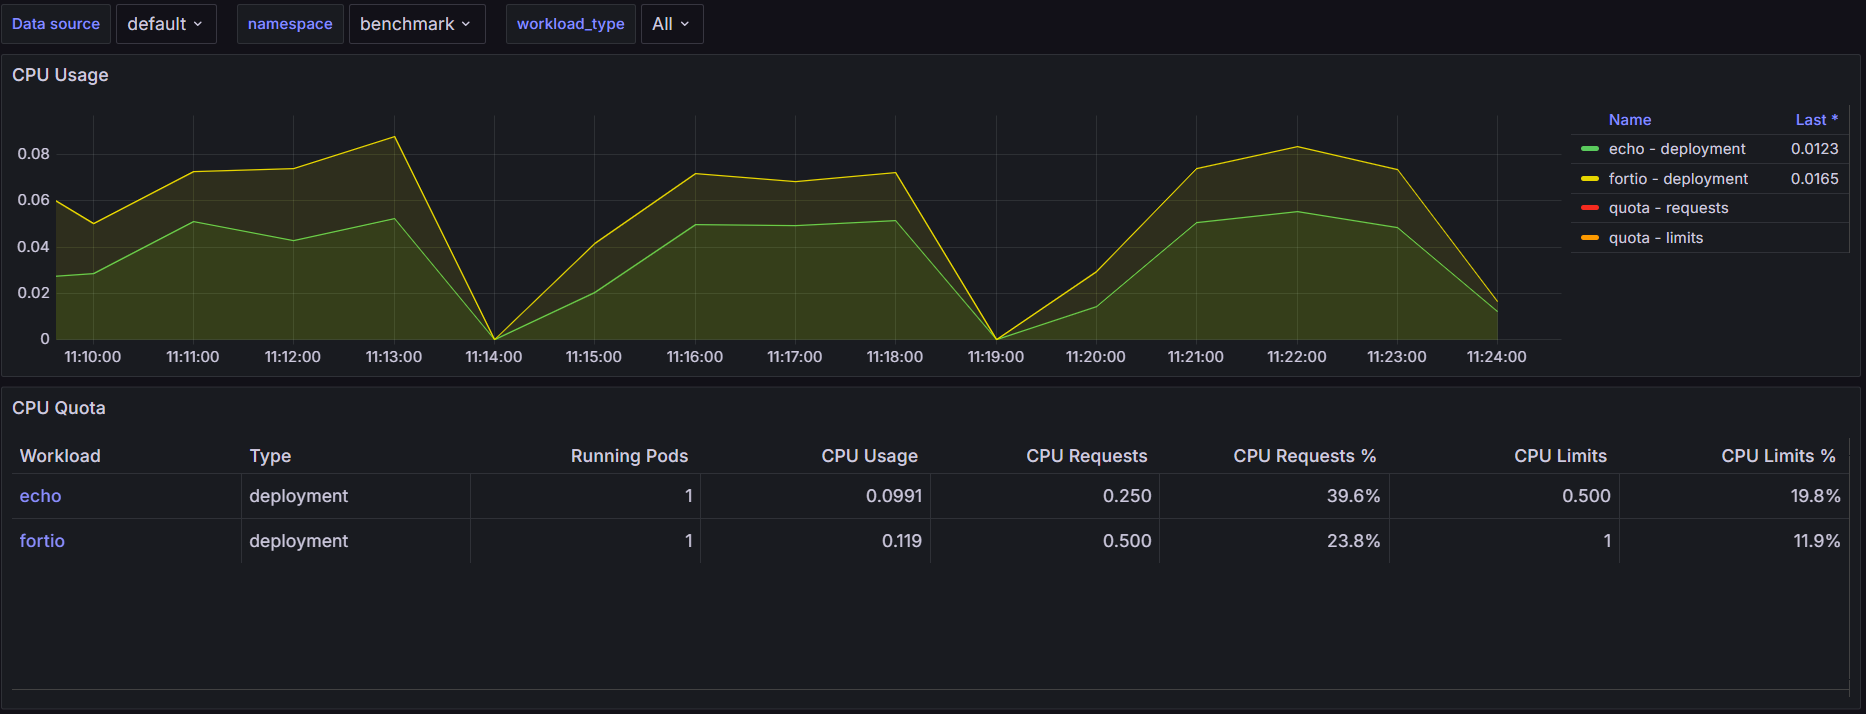
\includegraphics[width=0.88\textwidth]{../figures/grafana/modeA/grafana-ns-cpu-S2-L3-R1.png}
    \vspace{0.5em}
    
    \textbf{Mode B -- CPU namespace}\\[0.25em]
    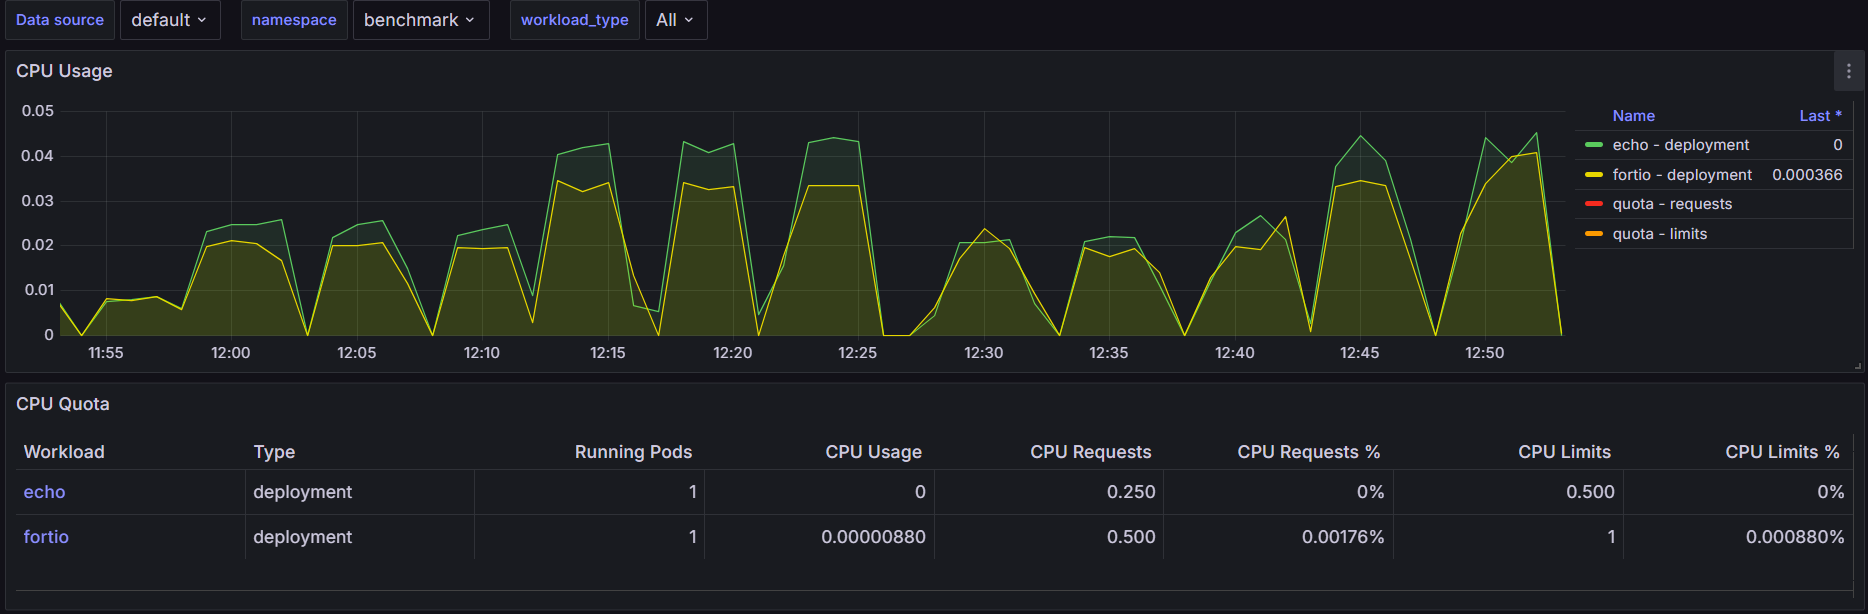
\includegraphics[width=0.88\textwidth]{../figures/grafana/modeB/grafana-ns-cpu-S2-L3.png}
    \caption{Bằng chứng Grafana namespace-level về CPU cho S2 L3 ở Mode A và Mode B; ảnh dùng như sanity check về resource pressure, không thay thế phân tích p99 theo pha}
    \label{fig:s2-grafana-cpu-evidence}
\end{figure}

\begin{figure}[H]
    \centering
    \textbf{Mode A -- memory namespace}\\[0.25em]
    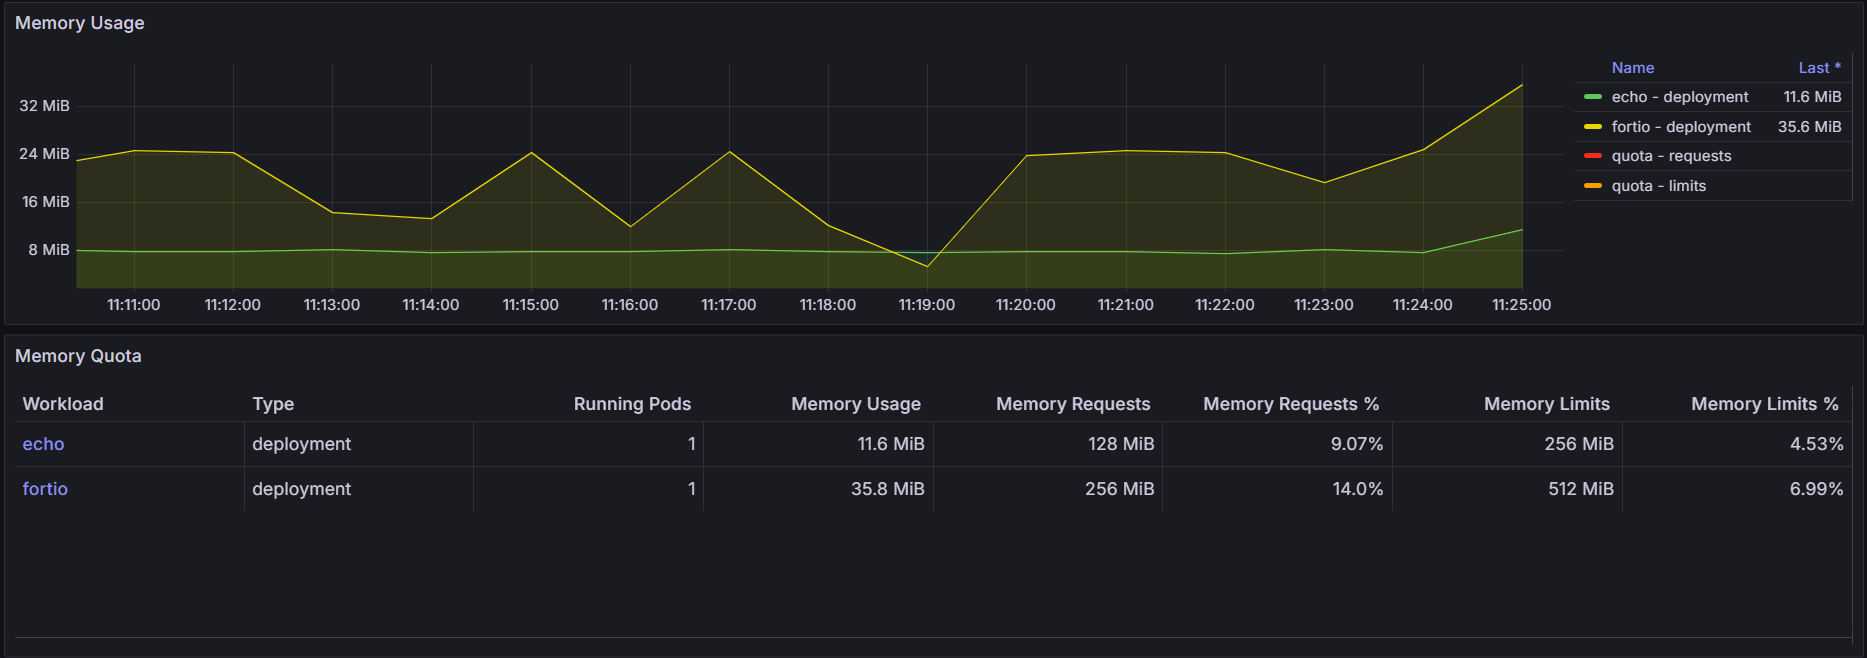
\includegraphics[width=0.88\textwidth]{../figures/grafana/modeA/grafana-ns-mem-S2-L3-R1.png}
    \vspace{0.5em}

    \textbf{Mode B -- memory namespace}\\[0.25em]
    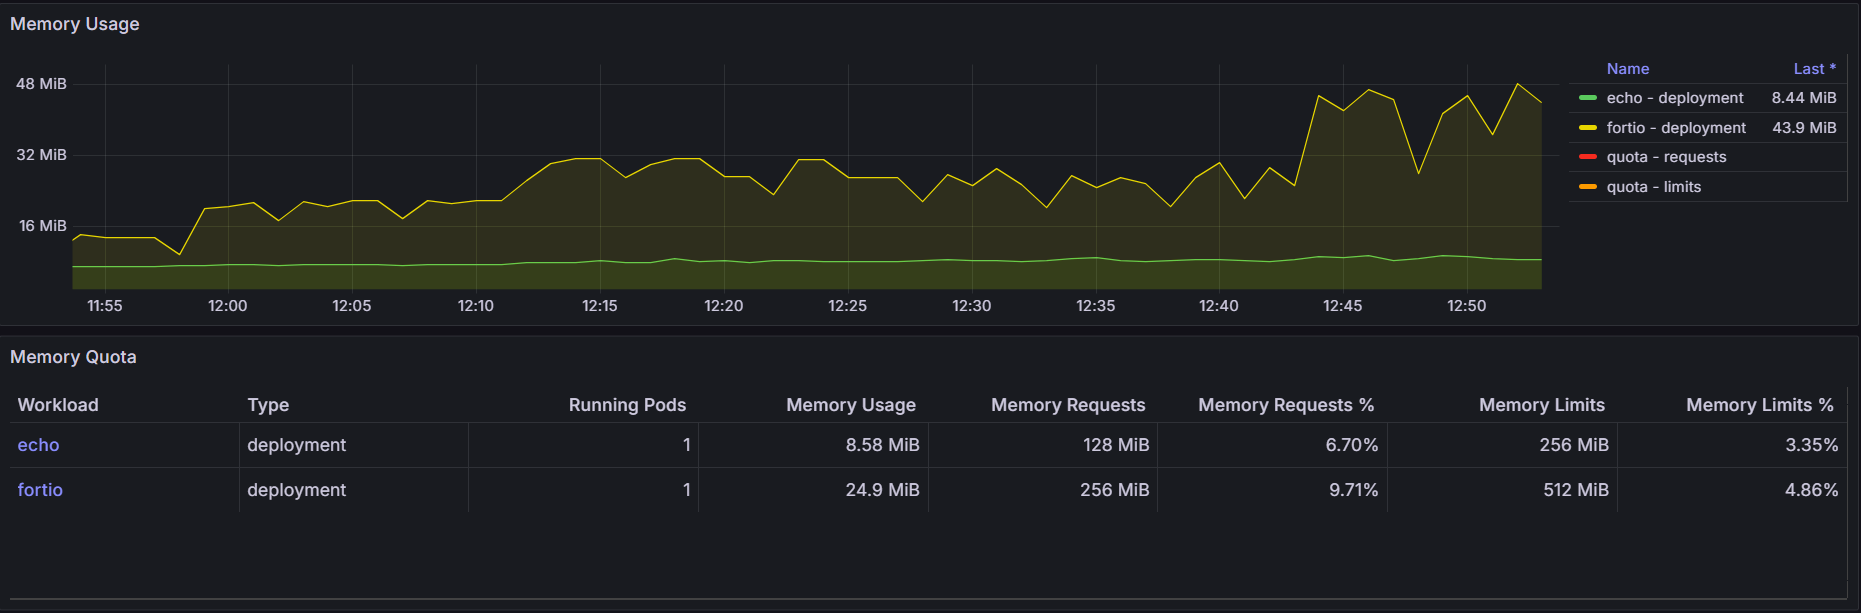
\includegraphics[width=0.88\textwidth]{../figures/grafana/modeB/grafana-ns-mem-S2-L3.png}
    \caption{Bằng chứng Grafana namespace-level về memory cho S2 L3 ở Mode A và Mode B; ảnh dùng như sanity check về resource pressure, không thay thế phân tích p99 theo pha}
    \label{fig:s2-grafana-memory-evidence}
\end{figure}

\textbf{Kết luận.} Với S2, kết luận an toàn là Mode B có xu hướng p99 tốt hơn rõ hơn ở L3, trong khi L2 vẫn có tính pha trộn. Kết quả này hỗ trợ nhận định về lợi thế datapath dưới tải cao và workload động, nhưng không đủ để khẳng định tuyệt đối cho mọi pha.

\section{Kết quả S3: chi phí NetworkPolicy}

S3 kiểm tra chi phí khi bật NetworkPolicy trong Mode B. Đây không phải là so sánh Mode A với Mode B; biến duy nhất được thay đổi là trạng thái policy OFF/ON trong cùng Mode B. Mục tiêu là xem một chính sách đơn giản có làm tăng p99 latency hoặc làm giảm achieved RPS đáng kể hay không.

Hai biểu đồ chính của S3 là p99 và achieved RPS khi policy OFF/ON. P99 cho biết tác động lên tail latency; RPS kiểm tra hai trạng thái vẫn được đo ở mức tải tương đương.

\begin{figure}[H]
    \centering
    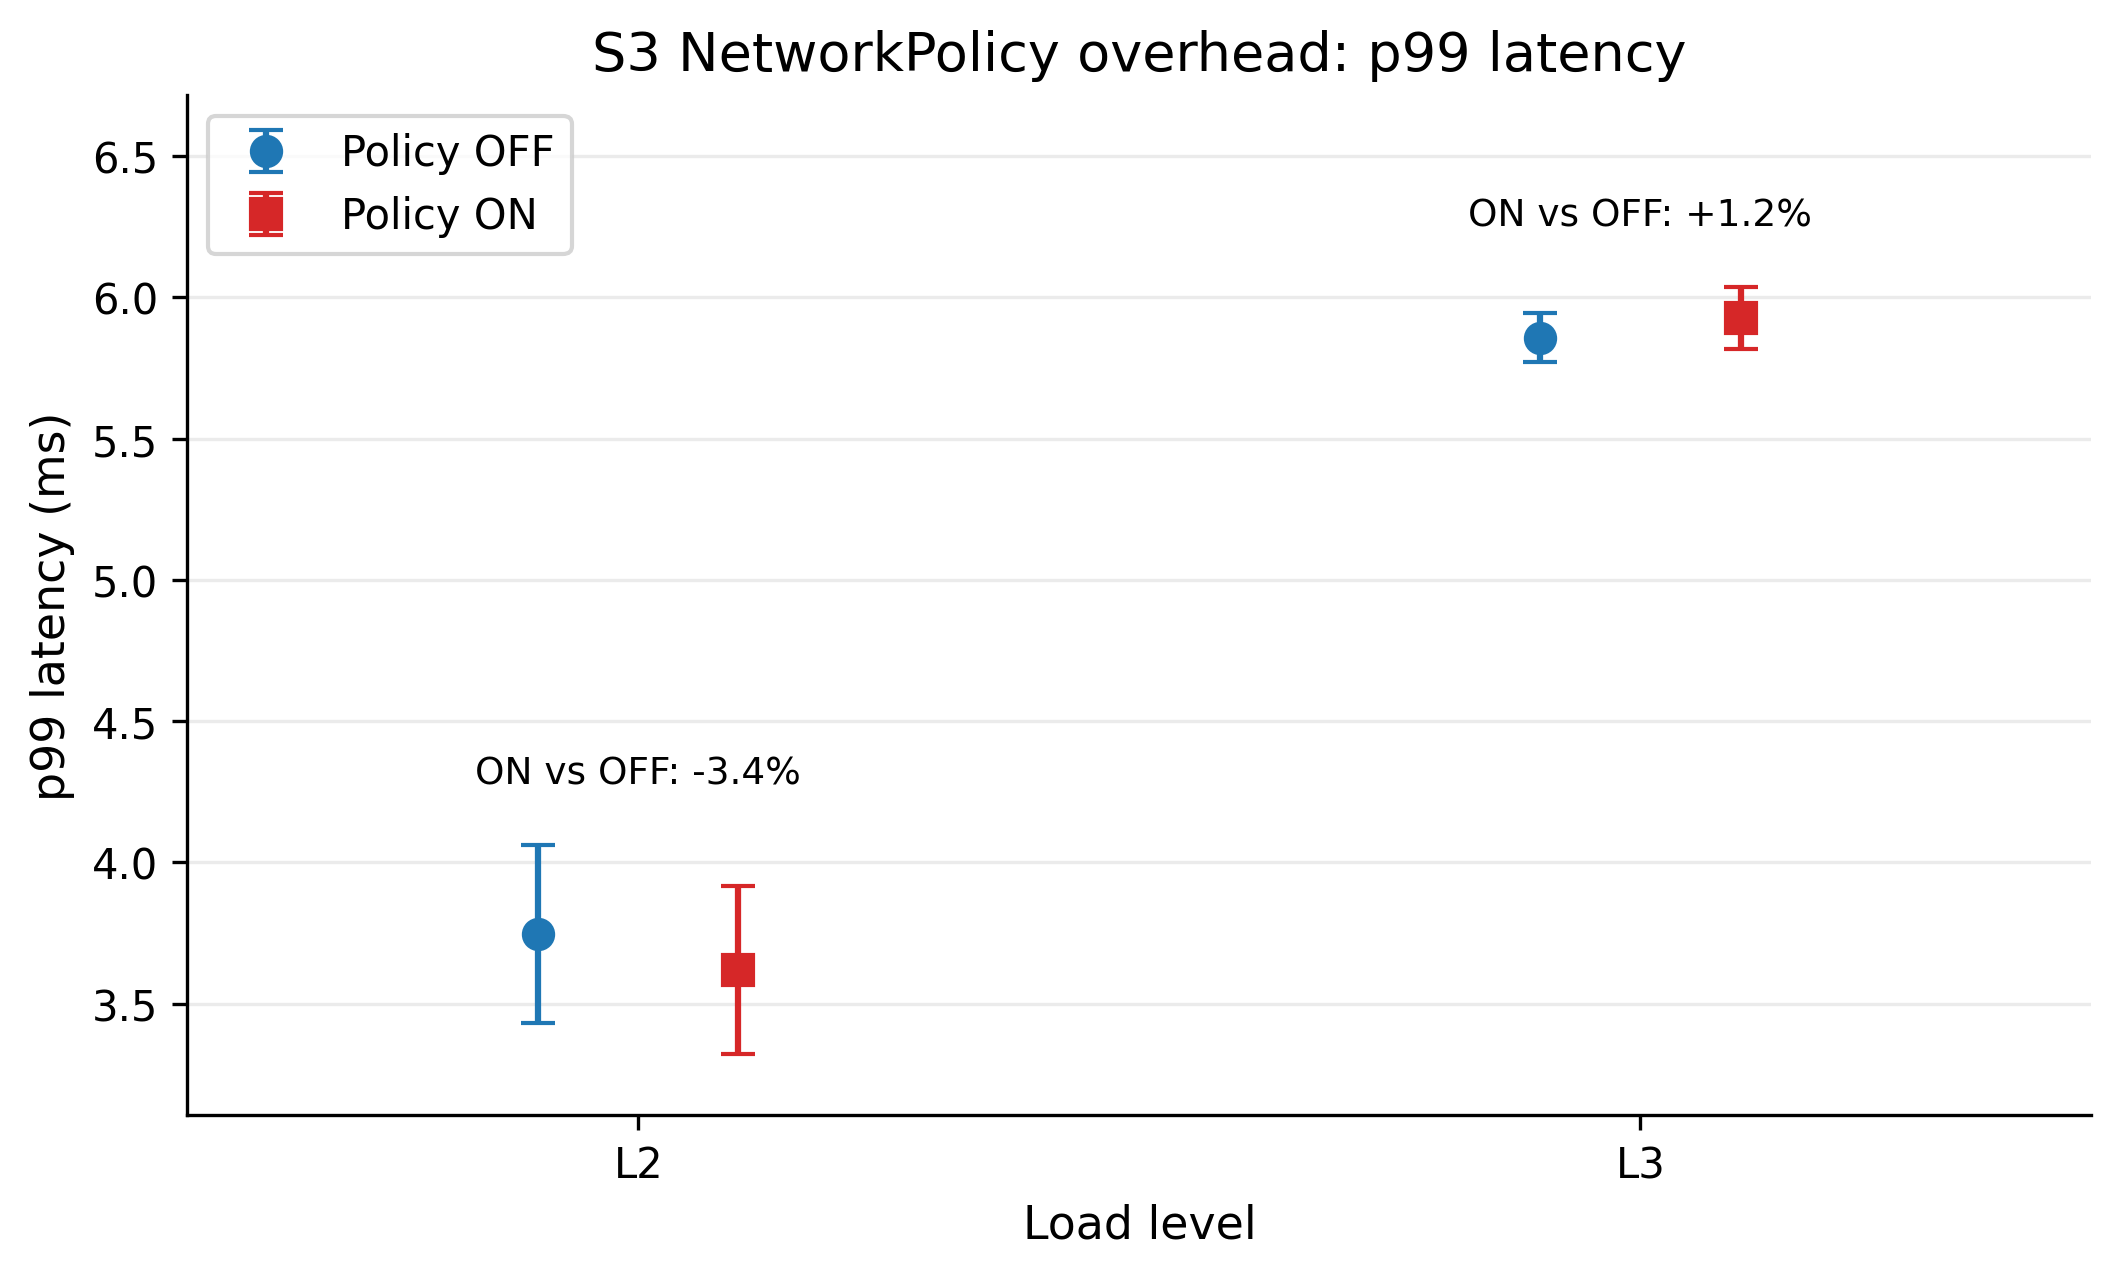
\includegraphics[width=0.82\textwidth]{../figures/thesis/fig-s3-policy-overhead-p99.png}
    \caption{P99 latency của S3 khi chính sách OFF và ON trong Mode B; các vạch dọc biểu diễn khoảng tin cậy 95\% quanh giá trị trung bình}
    \label{fig:s3-policy-overhead-p99}
\end{figure}

\begin{table}[H]
\centering
\caption{Tóm tắt kết quả S3 chính sách OFF và ON}
\label{tab:s3-policy-summary}
\renewcommand{\arraystretch}{1.2}
\begin{tabularx}{\textwidth}{>{\raggedright\arraybackslash}p{1.1cm}>{\raggedright\arraybackslash}p{1.4cm}>{\raggedleft\arraybackslash}p{1.8cm}>{\raggedleft\arraybackslash}p{3.0cm}>{\raggedleft\arraybackslash}p{1.9cm}>{\raggedleft\arraybackslash}X}
\toprule
\textbf{Tải} & \textbf{Policy} & \textbf{p99 mean} & \textbf{CI 95\%} & \textbf{RPS mean} & \textbf{Lỗi} \\
\midrule
L2 & OFF & 3.747 ms & 3.431--4.063 ms & 399.992 & 0.0\% \\
L2 & ON & 3.619 ms & 3.323--3.916 ms & 399.992 & 0.0\% \\
L3 & OFF & 5.857 ms & 5.770--5.944 ms & 799.974 & 0.0\% \\
L3 & ON & 5.928 ms & 5.818--6.037 ms & 799.965 & 0.0\% \\
\bottomrule
\end{tabularx}
\end{table}

\textbf{Phân tích.} Kết quả p99 cho thấy OFF và ON rất gần nhau. Ở L2, ON thấp hơn OFF một lượng nhỏ, nhưng không nên hiểu rằng policy làm tăng hiệu năng. Ở L3, ON cao hơn OFF khoảng 0.071 ms, tương đương khoảng 1.2\%; đây là mức chênh nhỏ về mặt thực tế. Các vạch CI 95\% cũng gần nhau, nên không có cơ sở để kết luận overhead p99 lớn trong dataset hiện tại.

\begin{figure}[H]
    \centering
    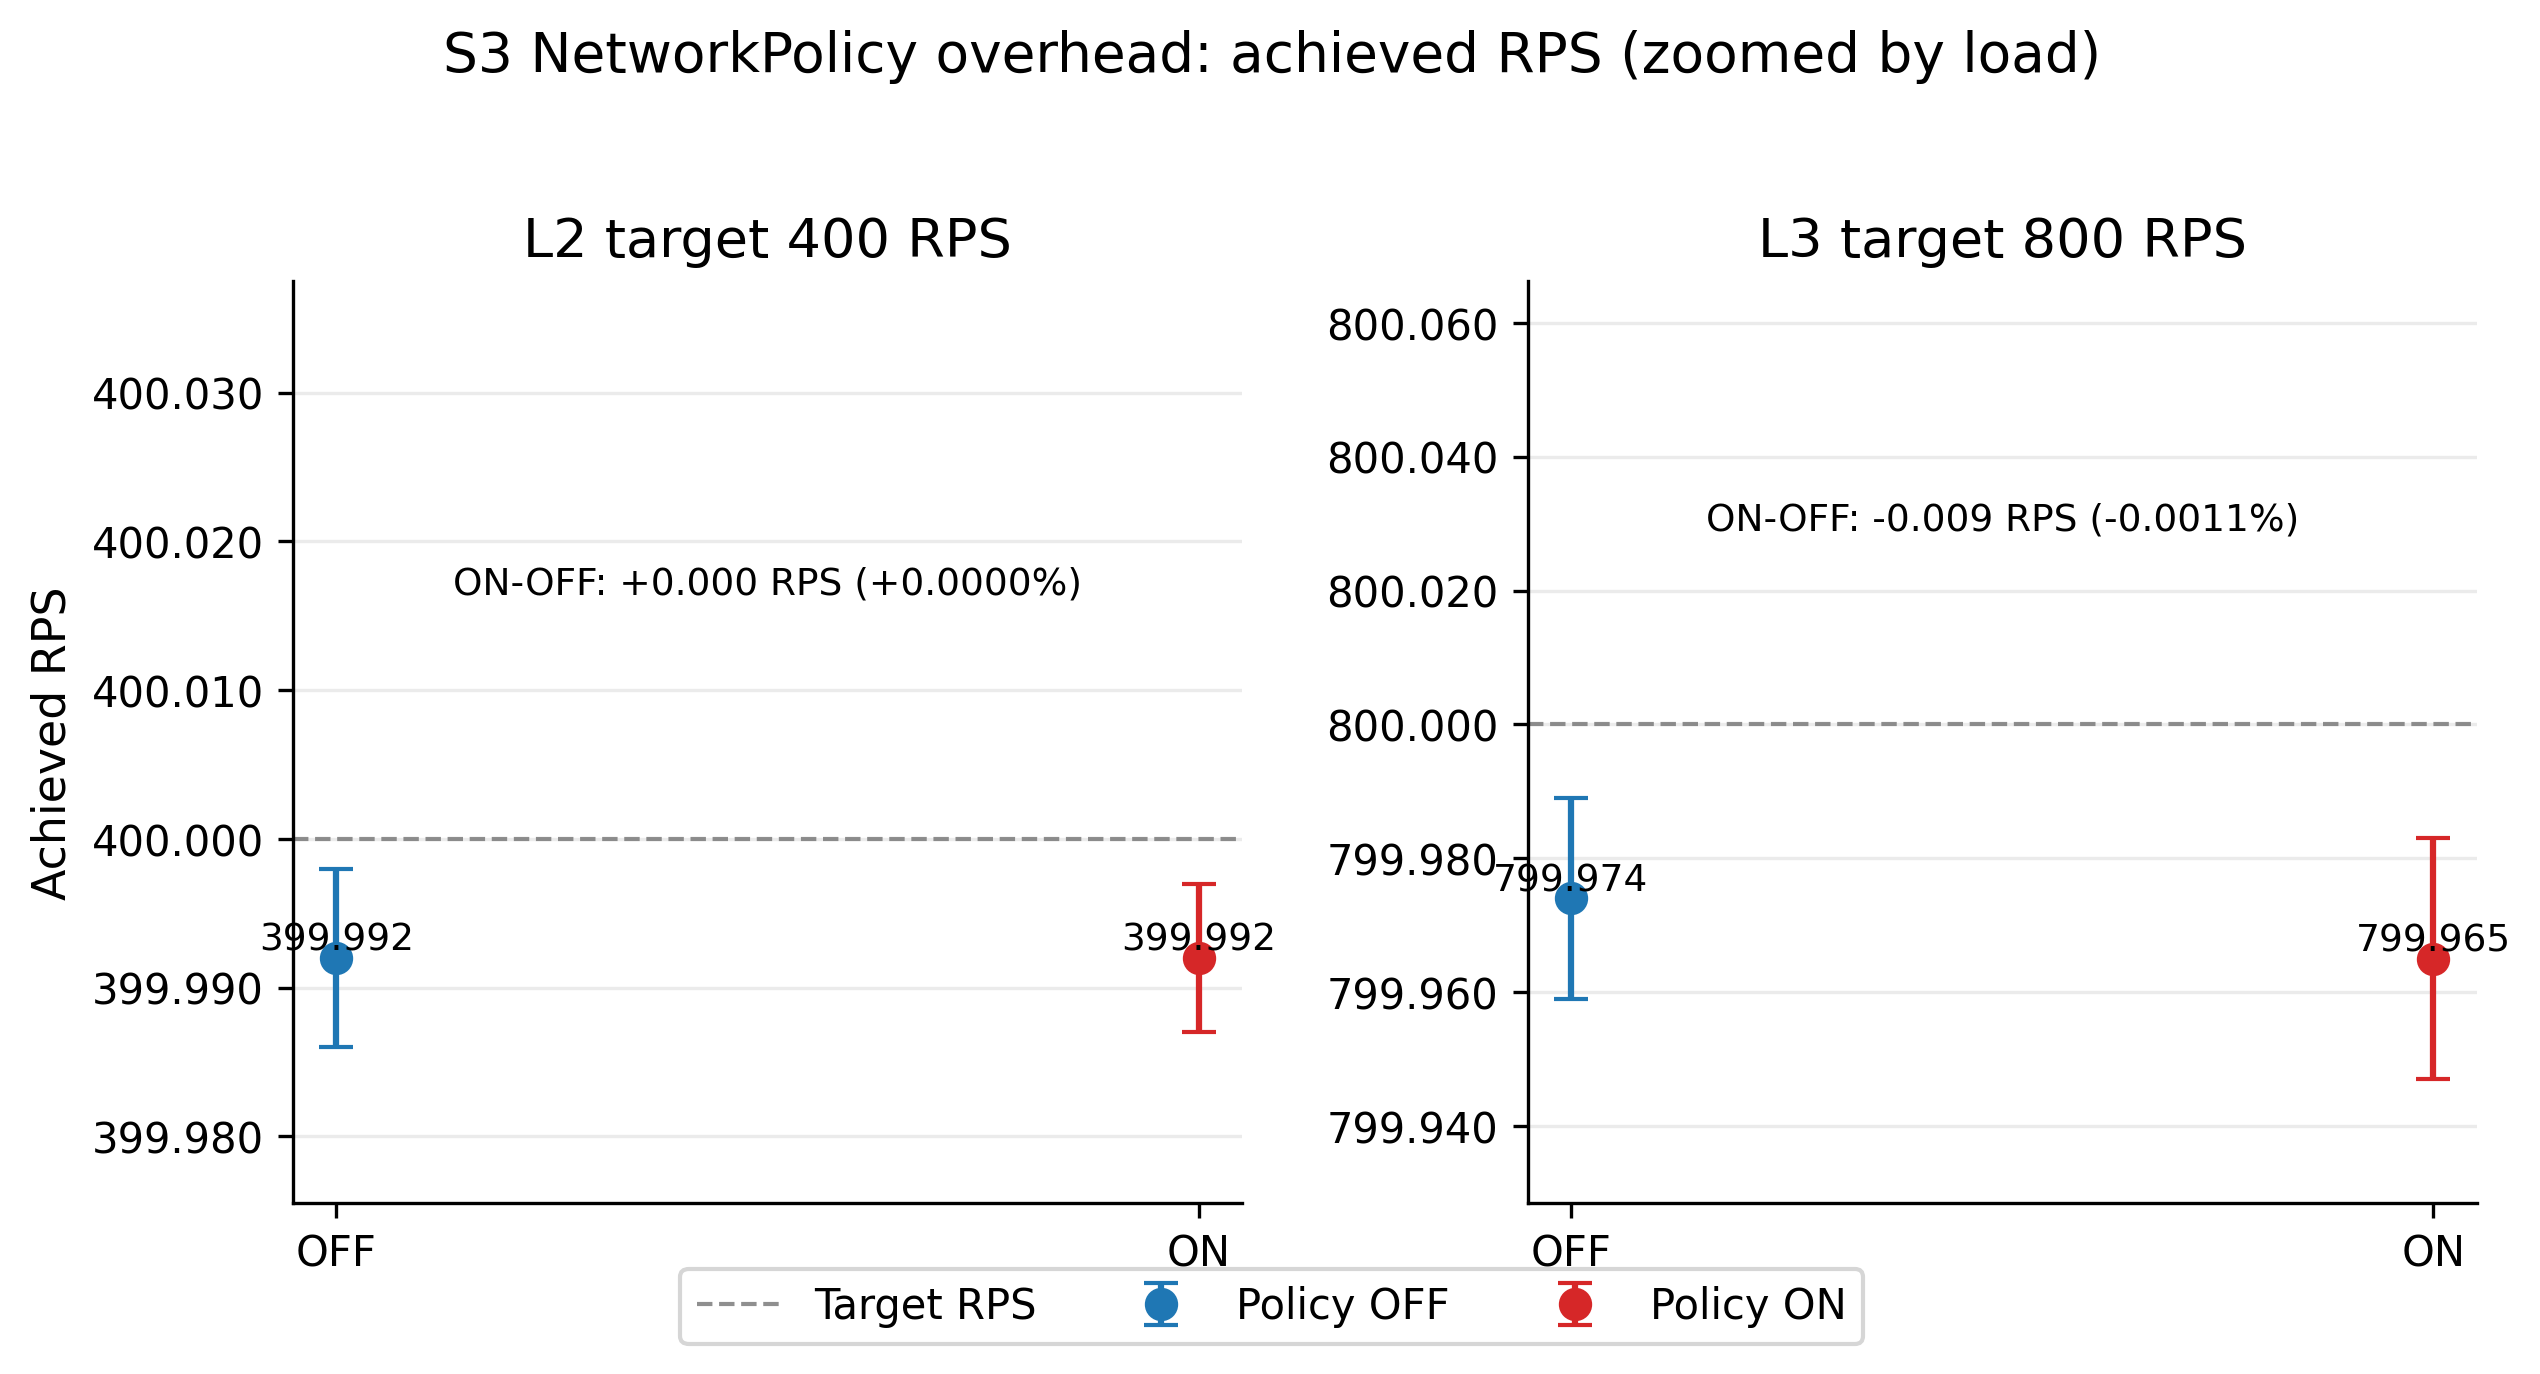
\includegraphics[width=0.82\textwidth]{../figures/thesis/fig-s3-policy-overhead-rps.png}
    \caption{RPS đạt được của S3 khi chính sách OFF và ON trong Mode B; các vạch dọc biểu diễn khoảng tin cậy 95\% quanh giá trị trung bình}
    \label{fig:s3-policy-overhead-rps}
\end{figure}

Hình~\ref{fig:s3-policy-overhead-rps} cho thấy achieved RPS gần như không đổi giữa OFF và ON, còn error rate bằng 0\%. Khi đọc cùng p99, cách diễn giải phù hợp là overhead quan sát được nhỏ. Tuy nhiên, error rate bằng 0\% chỉ nói rằng request hoàn tất thành công; nó không chứng minh policy enforcement không có chi phí.

Về cơ chế, kết quả OFF/ON gần nhau là hợp lý với policy đơn giản, số endpoint nhỏ và traffic benchmark đều được cho phép. Hình~\ref{fig:s3-hubble-policy-evidence} bổ sung bằng chứng Hubble ở mức flow/verdict: forward-case cho thấy flow được \texttt{forwarded}, còn deny-case thủ công minh họa verdict \texttt{Policy denied}.

Hubble chỉ là evidence bổ trợ về policy enforcement và observability. Kết luận overhead vẫn dựa trên p99, RPS và error rate từ Fortio. Các ảnh Hubble phụ khác được đặt ở Phụ lục~E.

\begin{figure}[H]
    \centering
    \textbf{Forward-case trong namespace benchmark}\\[0.25em]
    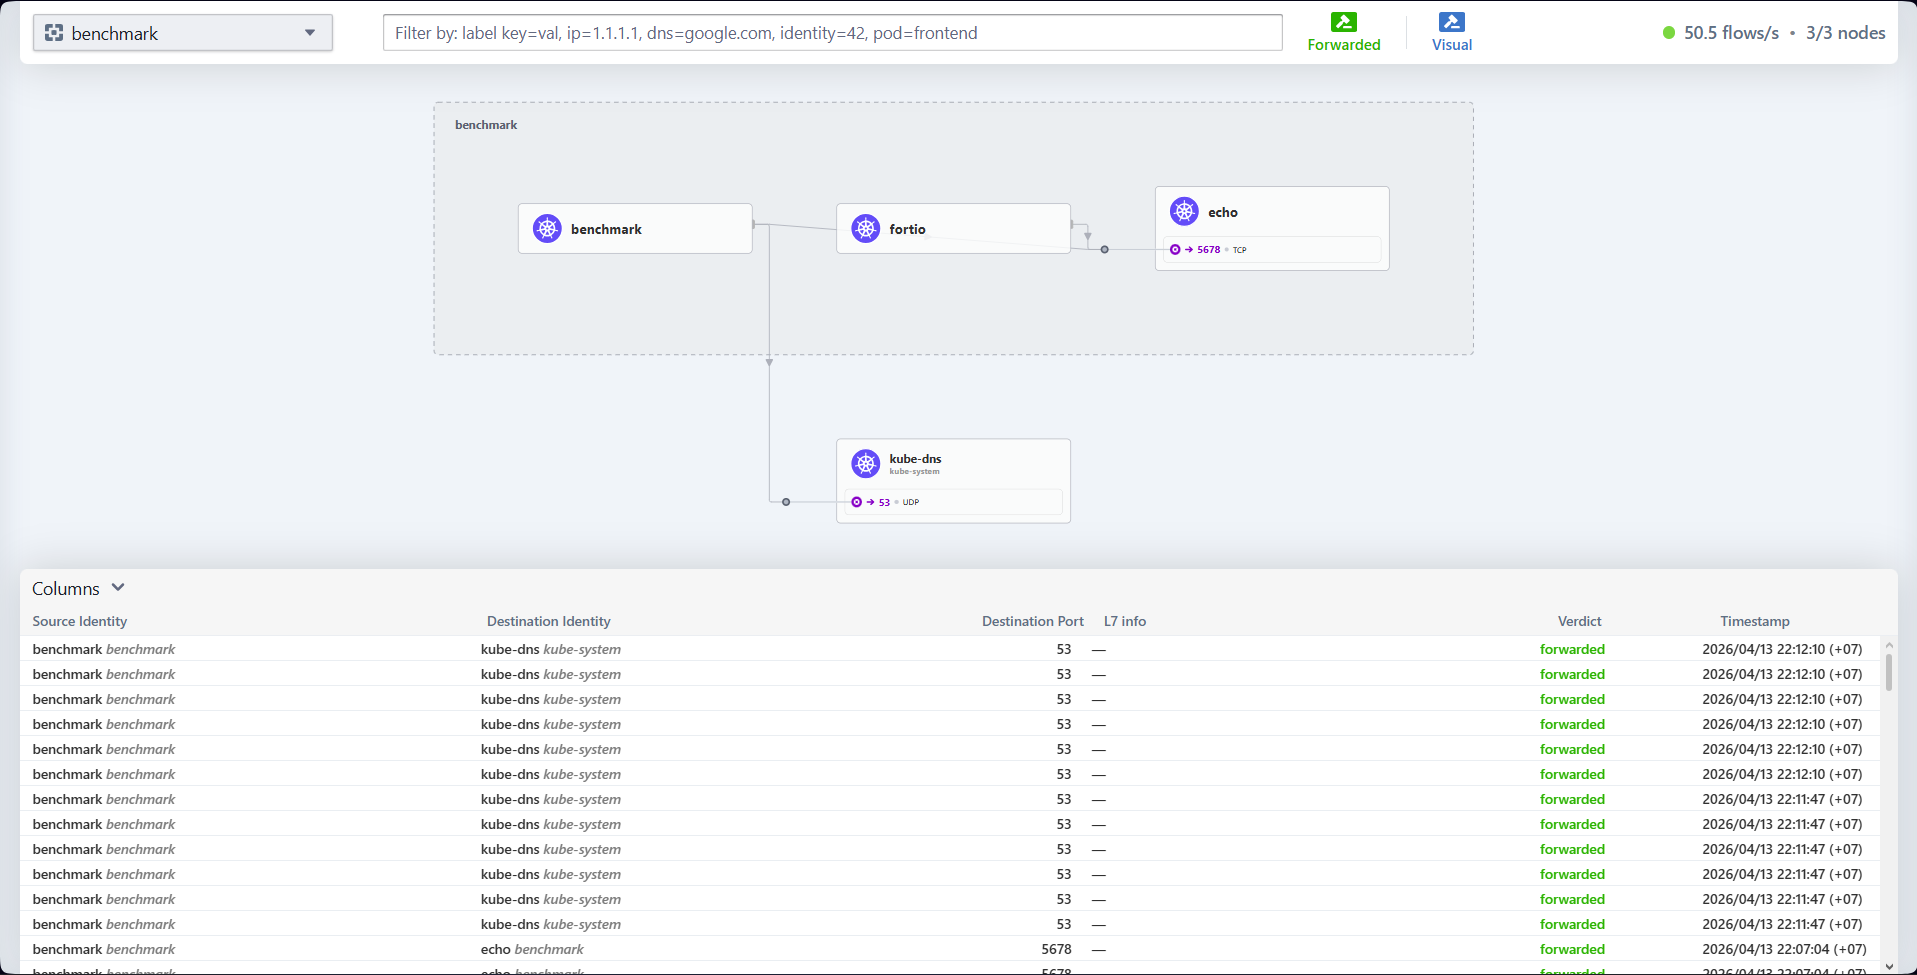
\includegraphics[width=0.86\textwidth]{../figures/hubble/fig-13b-hubble-forwarded-case.png}
    \vspace{0.4em}
    
    \textbf{Manual deny-case với Policy denied}\\[0.25em]
    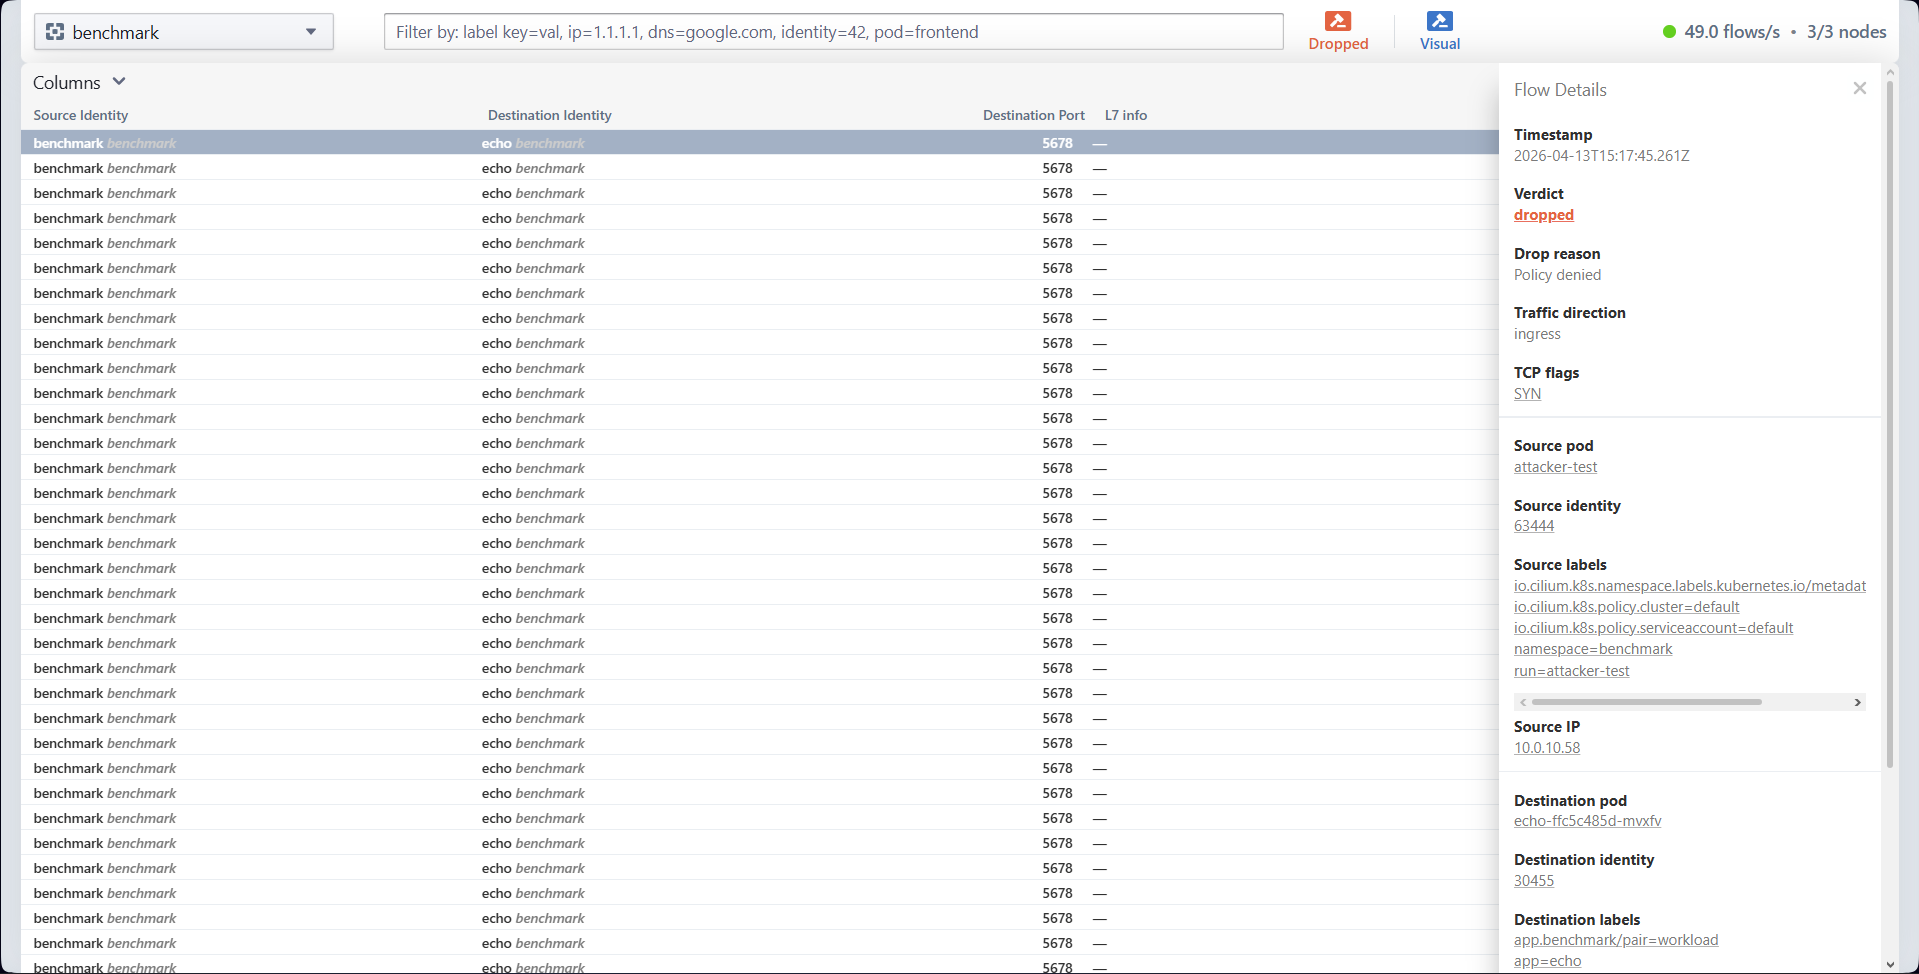
\includegraphics[width=0.86\textwidth]{../figures/hubble/fig13-hubble-deny-case-detail.png}
    \caption{Bằng chứng Hubble hỗ trợ cho S3 trong Mode B: forward-case với các flow được forwarded và manual deny-case với verdict policy denied; đây là evidence observability, không phải metric hiệu năng chính}
    \label{fig:s3-hubble-policy-evidence}
\end{figure}

\textbf{Kết luận.} Trong Mode B, với policy đơn giản và workload hiện tại, policy ON không tạo thay đổi p99 hoặc RPS đáng kể so với policy OFF. Kết luận này chỉ áp dụng cho setup đã đo và không nên khái quát cho policy phức tạp hơn.

\section{Độ lặp lại và tính ổn định}

Độ lặp lại giúp kiểm tra liệu kết luận có bị chi phối bởi một run cá biệt hay không. Hình~\ref{fig:repeatability-p99-dotplot} biểu diễn p99 của từng run cho các nhóm đại diện; mỗi điểm là một run thô, còn các vạch ngang ngắn là trung bình của nhóm, không phải khoảng tin cậy.

\begin{figure}[H]
    \centering
    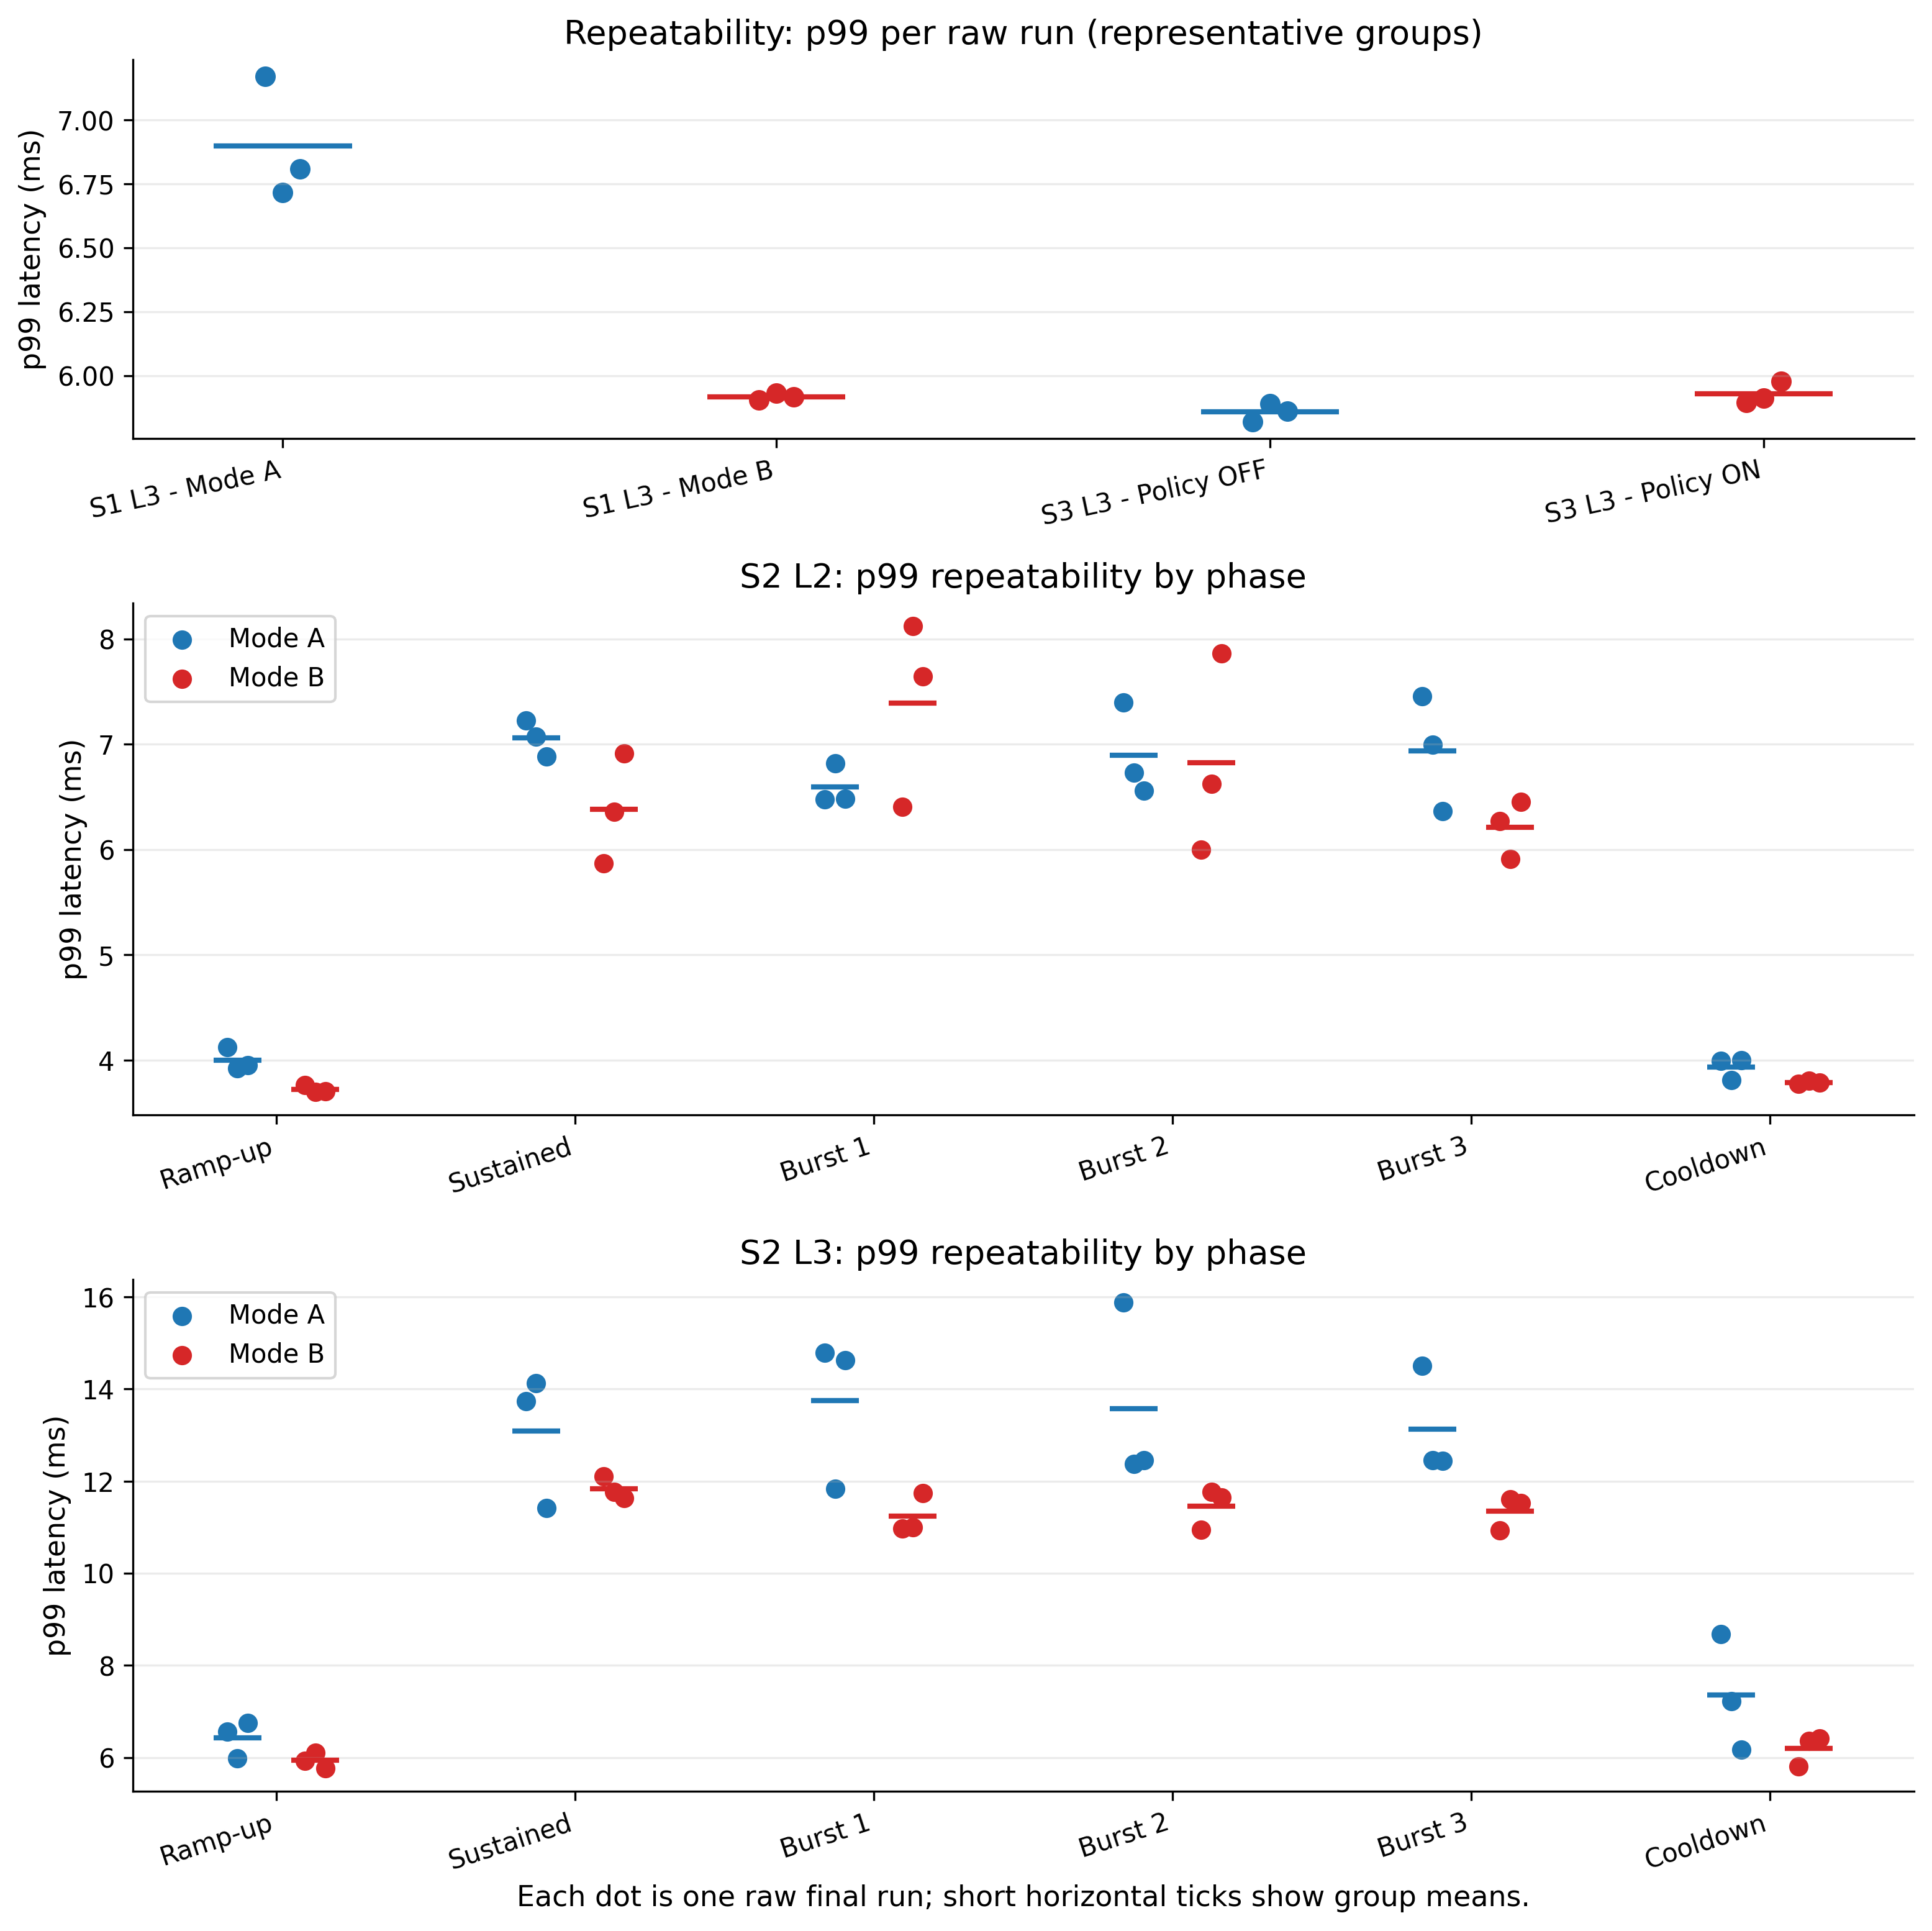
\includegraphics[width=0.90\textwidth]{../figures/thesis/fig-repeatability-p99-dotplot.png}
    \caption{Độ lặp lại p99 qua từng lần chạy; mỗi điểm là một run thô và vạch ngang ngắn là trung bình nhóm, không phải khoảng tin cậy}
    \label{fig:repeatability-p99-dotplot}
\end{figure}

\textbf{Phân tích.} CV\% mô tả dao động tương đối giữa các run. Ở S1 L3, Mode B vừa có p99 trung bình thấp hơn Mode A, vừa có CV thấp hơn; vì vậy, kết quả S1 có độ ổn định tốt hơn trong tập run hiện tại. Ở S3 L3, policy OFF và ON cũng có CV thấp, phù hợp với nhận định chênh lệch OFF/ON nhỏ.

Ngược lại, S2 biến động hơn do phase ngắn, burst và connection churn. Vì vậy, S1 và S3 có thể được diễn giải chắc hơn, còn S2 cần giữ ngôn ngữ thận trọng. Với \(n=3\), CV\% không làm tăng sức mạnh thống kê, nhưng giúp minh bạch chất lượng phép đo.

\textbf{Kết luận.} Độ lặp lại không thay thế kiểm định thống kê, nhưng giúp người đọc thấy nhóm nào ổn định hơn và nhóm nào cần diễn giải dè dặt. Đây là lý do mạch diễn giải của S1/S3 có thể chắc hơn, còn S2 nên được trình bày như xu hướng phụ thuộc pha.

\section{So sánh tổng hợp}

Bảng~\ref{tab:scenario-synthesis} tổng hợp vai trò của từng kịch bản, kết quả chính và caveat quan trọng nhất. Bảng này giúp liên kết các kịch bản thành một bức tranh chung, nhưng không thay thế phân tích chi tiết ở các mục trước.

\begin{table}[H]
\centering
\caption{Tổng hợp kết quả theo kịch bản}
\label{tab:scenario-synthesis}
\scriptsize
\setlength{\tabcolsep}{2.5pt}
\renewcommand{\arraystretch}{1.28}
\begin{tabularx}{\textwidth}{>{\raggedright\arraybackslash}p{2.0cm}>{\raggedright\arraybackslash}p{3.0cm}>{\raggedright\arraybackslash}X>{\raggedright\arraybackslash}p{3.0cm}}
\toprule
\textbf{Kịch bản} & \textbf{Mục tiêu} & \textbf{Kết quả chính} & \textbf{Caveat chính} \\
\midrule
Hiệu chuẩn & Chọn mức tải cuối & L1=100, L2=400, L3=800 QPS; L3 là tail-spike load, chưa phải saturation tuyệt đối & Error rate 0\% không có nghĩa là không có stress \\
S1 & So sánh Mode A và Mode B dưới tải ổn định & Mode B có p99 thấp hơn, rõ nhất ở L2 và L3 & L1 không significant; không khái quát ngoài môi trường đo \\
S2 & Kiểm tra burst, churn và hành vi theo pha & L3 cho xu hướng Mode B thấp hơn ở toàn bộ pha; L2 có kết quả pha trộn & Variance cao; Burst 1 L2 là ngoại lệ \\
S3 & Đo policy OFF/ON trong Mode B & Policy ON không làm p99 hoặc RPS thay đổi đáng kể trong dataset hiện tại & Chỉ áp dụng cho policy đơn giản và traffic hiện tại \\
Độ lặp lại & Kiểm tra độ ổn định giữa các run & S1/S3 ổn định hơn; S2 biến động hơn & \(n=3\) vẫn là giới hạn quan trọng \\
\bottomrule
\end{tabularx}
\end{table}

Nhìn tổng thể, S1 cung cấp bằng chứng sạch nhất về khác biệt datapath trong điều kiện ổn định. S2 cho thấy khác biệt phụ thuộc vào pha và mức tải. S3 tách riêng câu hỏi chi phí policy trong Mode B và cho thấy overhead quan sát được nhỏ với policy đơn giản. Độ lặp lại giúp xác định nhóm kết quả nào có thể viết chắc hơn và nhóm nào chỉ nên xem là xu hướng.

\section{Phân tích theo RQ1, RQ2 và RQ3}

\subsection{RQ1: Mode B có cải thiện latency trong tải ổn định so với Mode A không?}

Câu trả lời ngắn gọn là có bằng chứng ủng hộ, đặc biệt tại L2 và L3. Trong S1, Mode B có p99 trung bình thấp hơn Mode A ở cả ba mức tải; L2 và L3 được đánh dấu significant, còn L1 chỉ nên xem là xu hướng. Vì vậy, trong điều kiện steady-state của benchmark hiện tại, Mode B cho thấy lợi thế tail latency rõ hơn ở tải trung bình và tải cao.

\subsection{RQ2: Khác biệt giữa hai mode thay đổi thế nào dưới burst và connection churn?}

Câu trả lời là khác biệt phụ thuộc vào pha và mức tải. Tại L2, Mode B có xu hướng tốt hơn ở nhiều pha nhưng Burst 1 là ngoại lệ. Tại L3, Mode B có p99 trung bình thấp hơn ở toàn bộ pha, đặc biệt trong các pha burst, nhưng chưa significant. Vì vậy, S2 ủng hộ nhận định Mode B có thể có lợi thế tail latency dưới tải cao và workload động, nhưng chưa đủ để khẳng định tốt hơn ở mọi pha.

\subsection{RQ3: Bật NetworkPolicy trong Mode B có tạo chi phí đáng kể không?}

Câu trả lời là trong tập dữ liệu hiện tại, chi phí quan sát được là nhỏ. Trong S3, policy ON không làm RPS giảm đáng kể và p99 chỉ thay đổi rất nhỏ so với OFF. Error rate bằng 0\% cho thấy workload hoàn tất thành công, nhưng không chứng minh overhead bằng không. Kết luận này chỉ áp dụng cho policy đơn giản và allowed traffic trong benchmark hiện tại.

\section{Tổng kết chương}

Chương này đã trình bày kết quả benchmark theo logic kịch bản: hiệu chuẩn tải, S1, S2, S3 và độ lặp lại. Mode B có lợi thế p99 rõ nhất trong S1 ở L2/L3; trong S2, xu hướng có lợi cho Mode B rõ hơn ở L3 nhưng phụ thuộc pha; trong S3, NetworkPolicy đơn giản trong Mode B không tạo overhead p99/RPS đáng kể trong dataset hiện tại.

Các kết luận trên cần được đọc trong phạm vi thực nghiệm của đề tài: EKS, 3 worker nodes \texttt{m5.large}, workload Fortio/HTTP echo, các mức tải L1/L2/L3, số lần lặp nhỏ và policy đơn giản. Chương 5 sẽ dùng các kết quả này để tổng hợp đóng góp, nêu giới hạn nghiên cứu và đề xuất hướng mở rộng.

% Chương 5: Conclusion

% ==========================================
% CHƯƠNG 5: CONCLUSION 
% ==========================================
\chapter{Conclusion}
\section{Summary of findings} % 
\section{Practical implications} % 
\section{Limitations} % 
\section{Future work} % 


% ==========================================
% PHỤ LỤC (APPENDICES) 
% ==========================================
\appendix
% Chi tiết hạ tầng
\chapter{Infrastructure Details} % 

% Dữ liệu calibration
\chapter{Calibration Data} % 

% Phương pháp thống kê
\chapter{Statistical Methods} % 

% Ánh xạ dữ liệu thô
\chapter{Raw Data Mapping} % 

% Hình bổ sung
\chapter{Hình bổ sung về telemetry và observability}

Phụ lục này tập hợp các ảnh Grafana/Prometheus và Hubble bổ sung cho phần phân tích ở Chương 4. Các ảnh trong phụ lục không phải là kết quả benchmark chính và không thay thế các biểu đồ p99, RPS, delta hoặc bảng thống kê. Vai trò của chúng là cung cấp thêm bối cảnh vận hành, hỗ trợ kiểm tra rằng các kết luận chính không bị chi phối bởi một dấu hiệu resource saturation hiển nhiên, đồng thời minh họa khả năng quan sát flow/verdict bằng Hubble trong Mode B.

Khi đọc các hình trong phụ lục, cần lưu ý rằng ảnh dashboard là snapshot theo cửa sổ thời gian, không phải time series đã được căn chỉnh chính xác với từng Fortio run hoặc từng pha trong S2. Vì vậy, chúng chỉ nên được dùng như bằng chứng hỗ trợ/sanity check, không dùng để kết luận định lượng về mức tiêu thụ CPU/memory của từng mode.

\section{Ảnh Grafana tổng quan}

Các ảnh tổng quan dưới đây minh họa các nhóm panel được dùng khi quan sát CPU, memory và network trong quá trình benchmark. Đây là cơ sở để đối chiếu bối cảnh vận hành, nhưng không phải nguồn chính để tính p99, RPS hoặc ý nghĩa thống kê.

\begin{figure}[H]
    \centering
    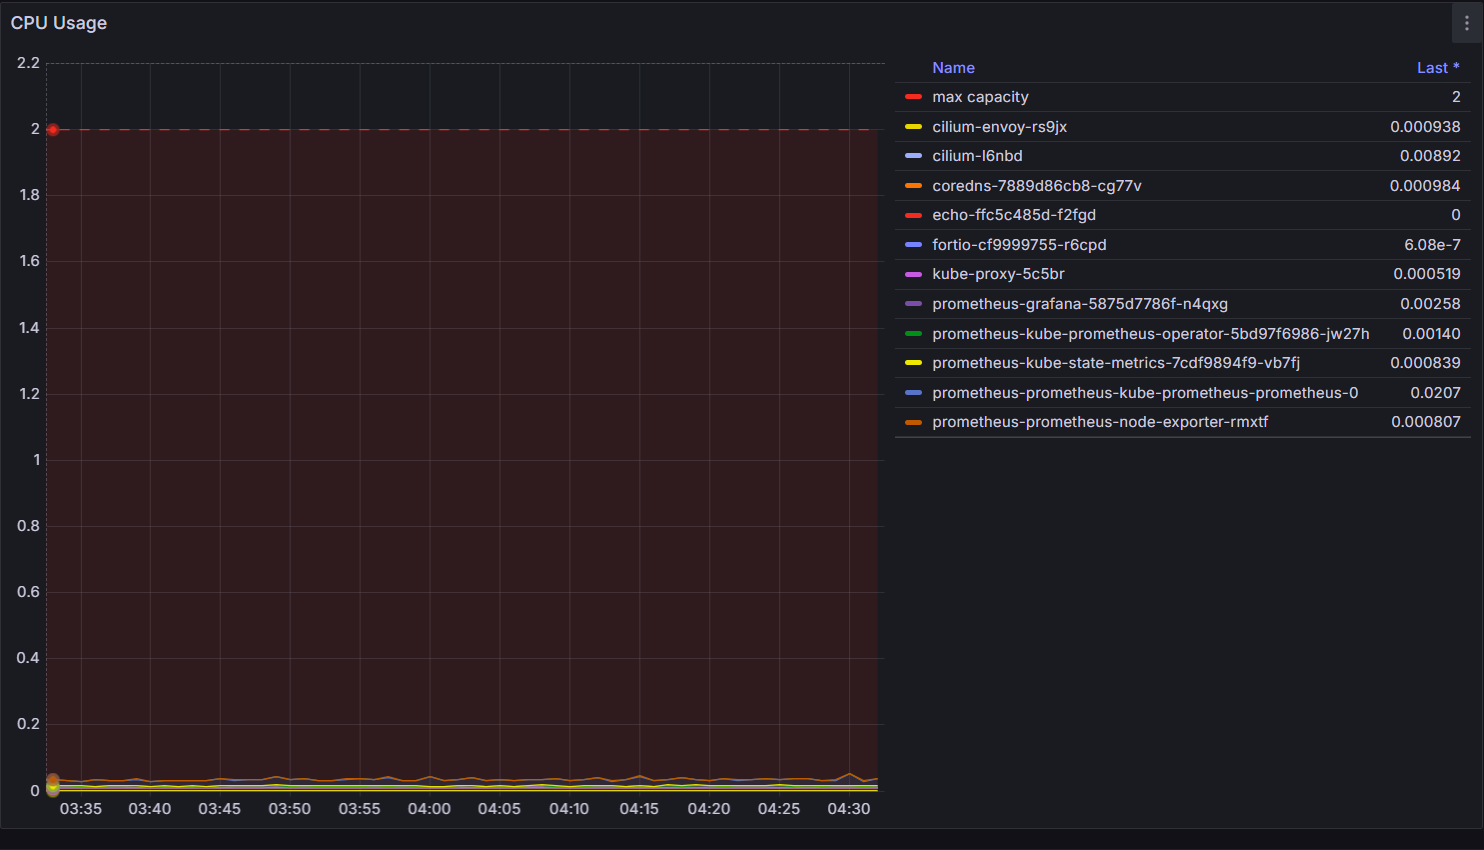
\includegraphics[width=0.92\textwidth]{../figures/grafana/fig-G1-grafana-cpu-node-pod.png}
    \caption{Panel Grafana/Prometheus tổng quan về CPU theo node/pod}
    \label{fig:app-grafana-cpu-node-pod}
\end{figure}

\begin{figure}[H]
    \centering
    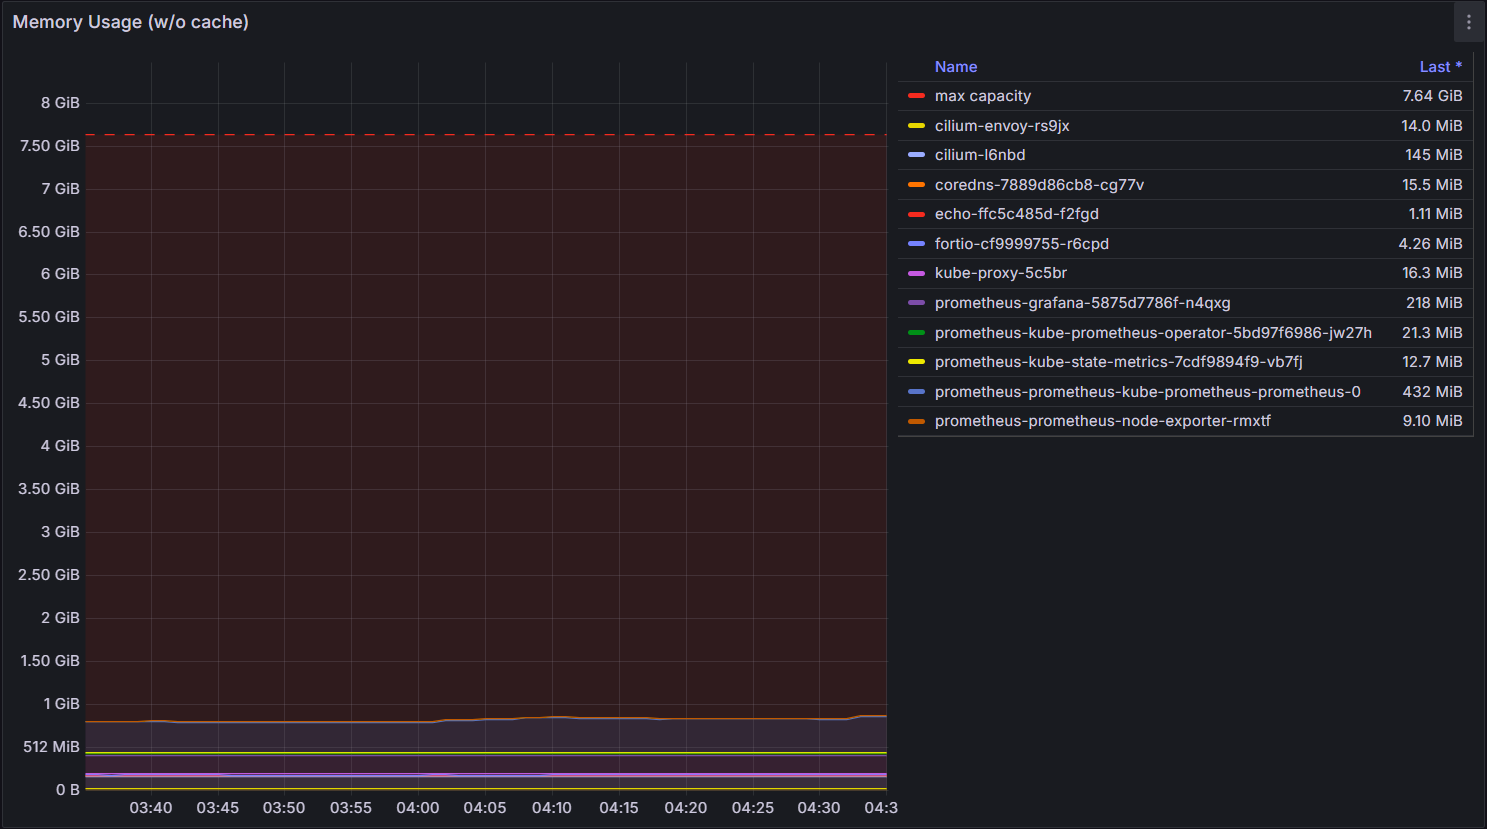
\includegraphics[width=0.92\textwidth]{../figures/grafana/fig-G3-grafana-memory-node-pod.png}
    \caption{Panel Grafana/Prometheus tổng quan về memory theo node/pod}
    \label{fig:app-grafana-memory-node-pod}
\end{figure}

\begin{figure}[H]
    \centering
    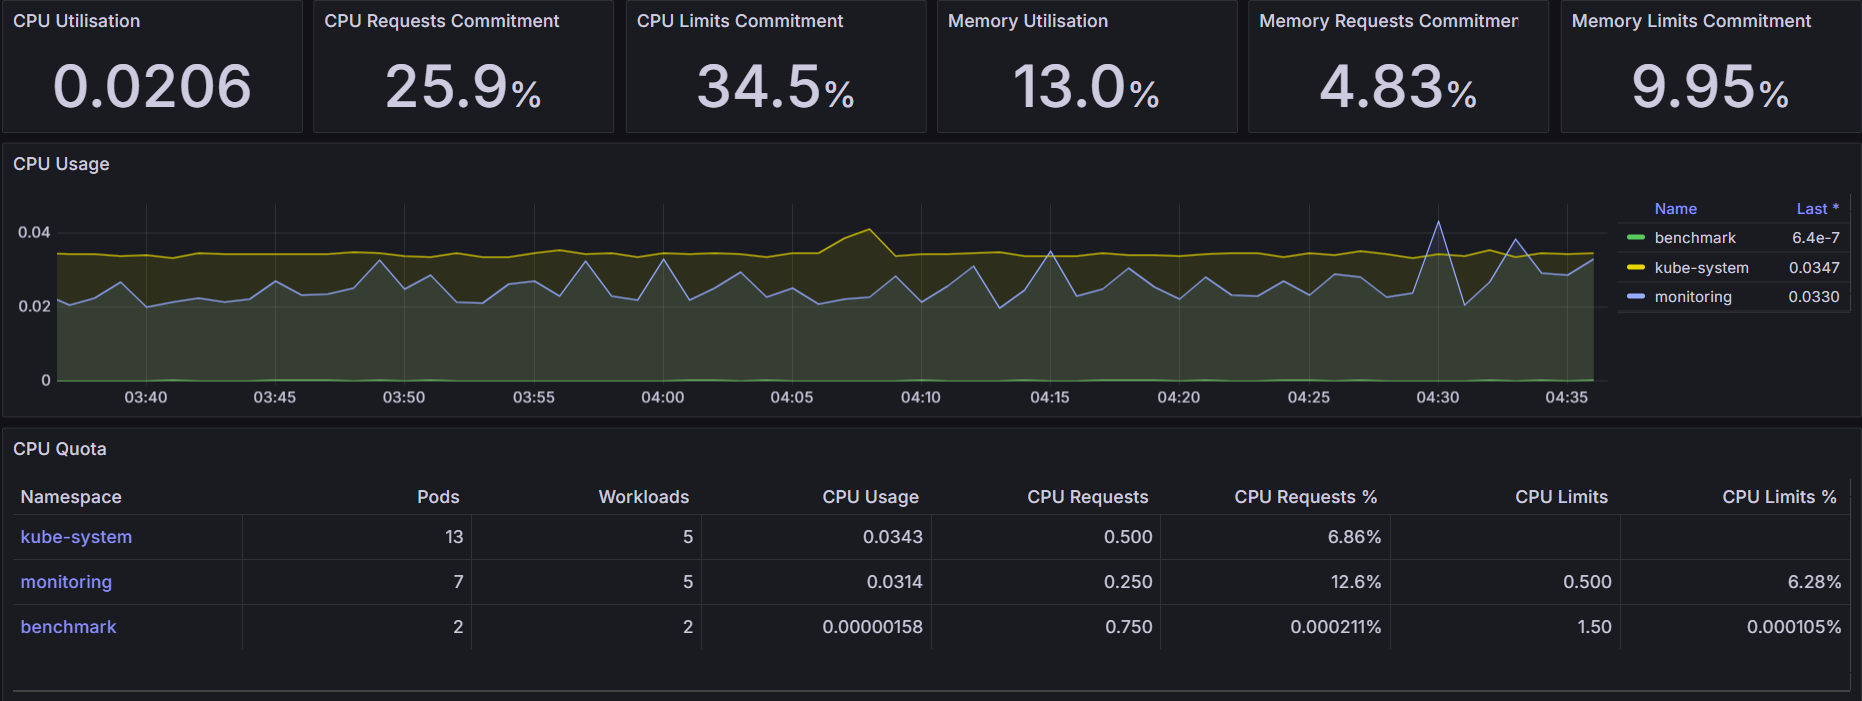
\includegraphics[width=0.92\textwidth]{../figures/grafana/fig-G4-grafana-cluster-overview.png}
    \caption{Panel Grafana/Prometheus tổng quan về trạng thái cluster}
    \label{fig:app-grafana-cluster-overview}
\end{figure}

\begin{figure}[H]
    \centering
    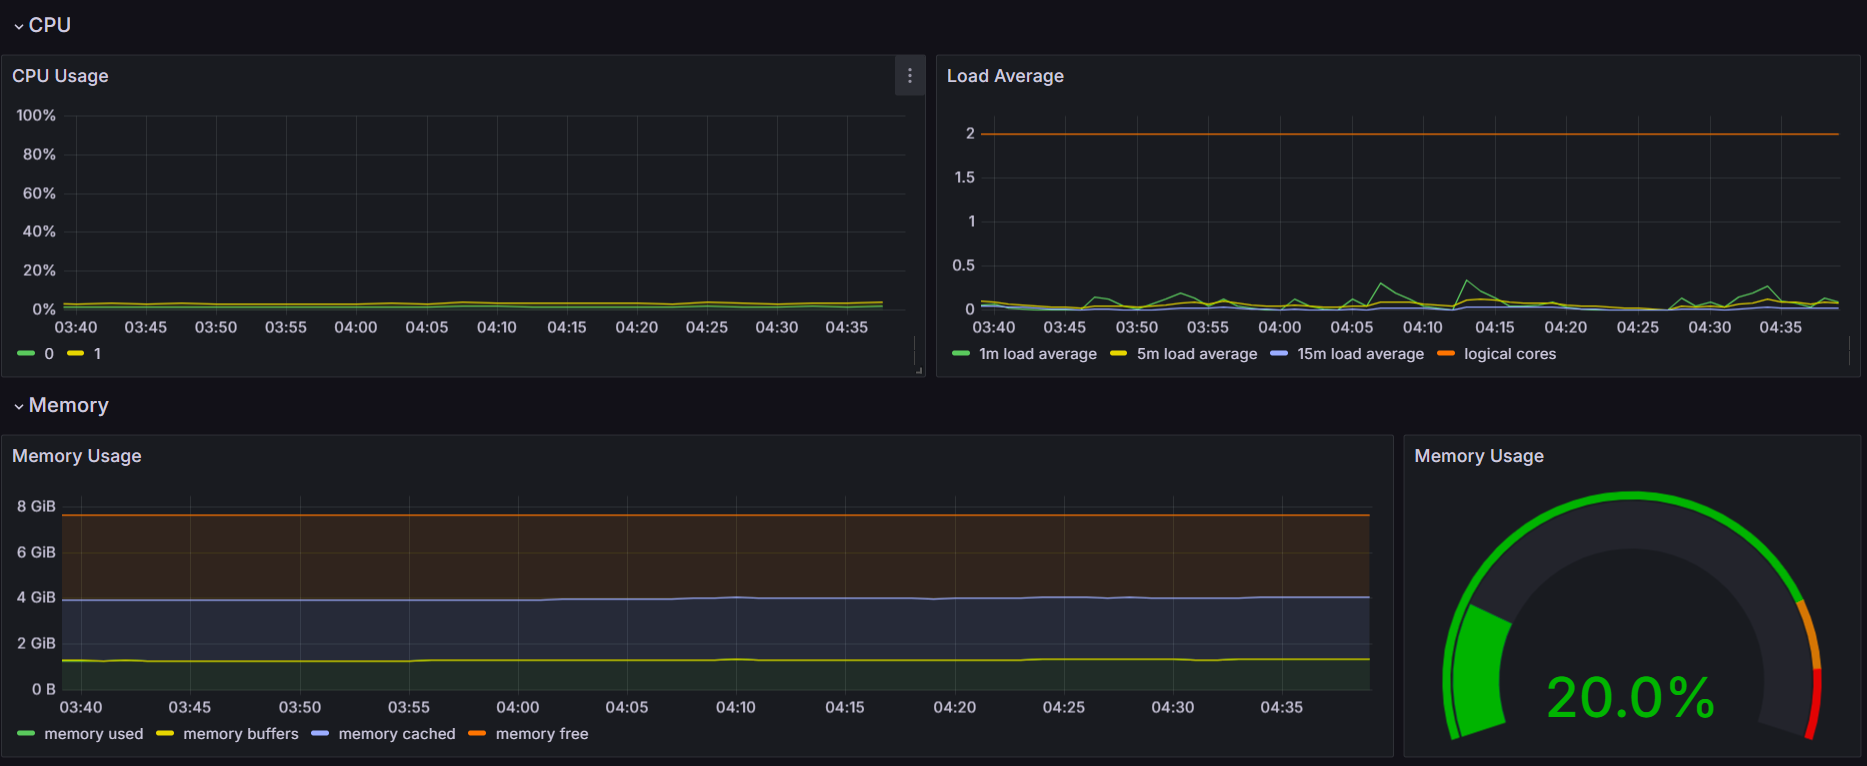
\includegraphics[width=0.92\textwidth]{../figures/grafana/fig-G5-grafana-node-network.png}
    \caption{Panel Grafana/Prometheus tổng quan về network theo node}
    \label{fig:app-grafana-node-network}
\end{figure}

\section{Ảnh Grafana bổ sung cho S1}

Các ảnh S1 L2 giúp kiểm tra bối cảnh CPU/memory ở mức namespace cho cả hai mode. Ảnh chính trong Chương 4 tập trung vào S1 L3 vì đó là mức tải có chênh lệch p99 rõ hơn; các ảnh dưới đây chỉ đóng vai trò bổ sung.

\begin{figure}[H]
    \centering
    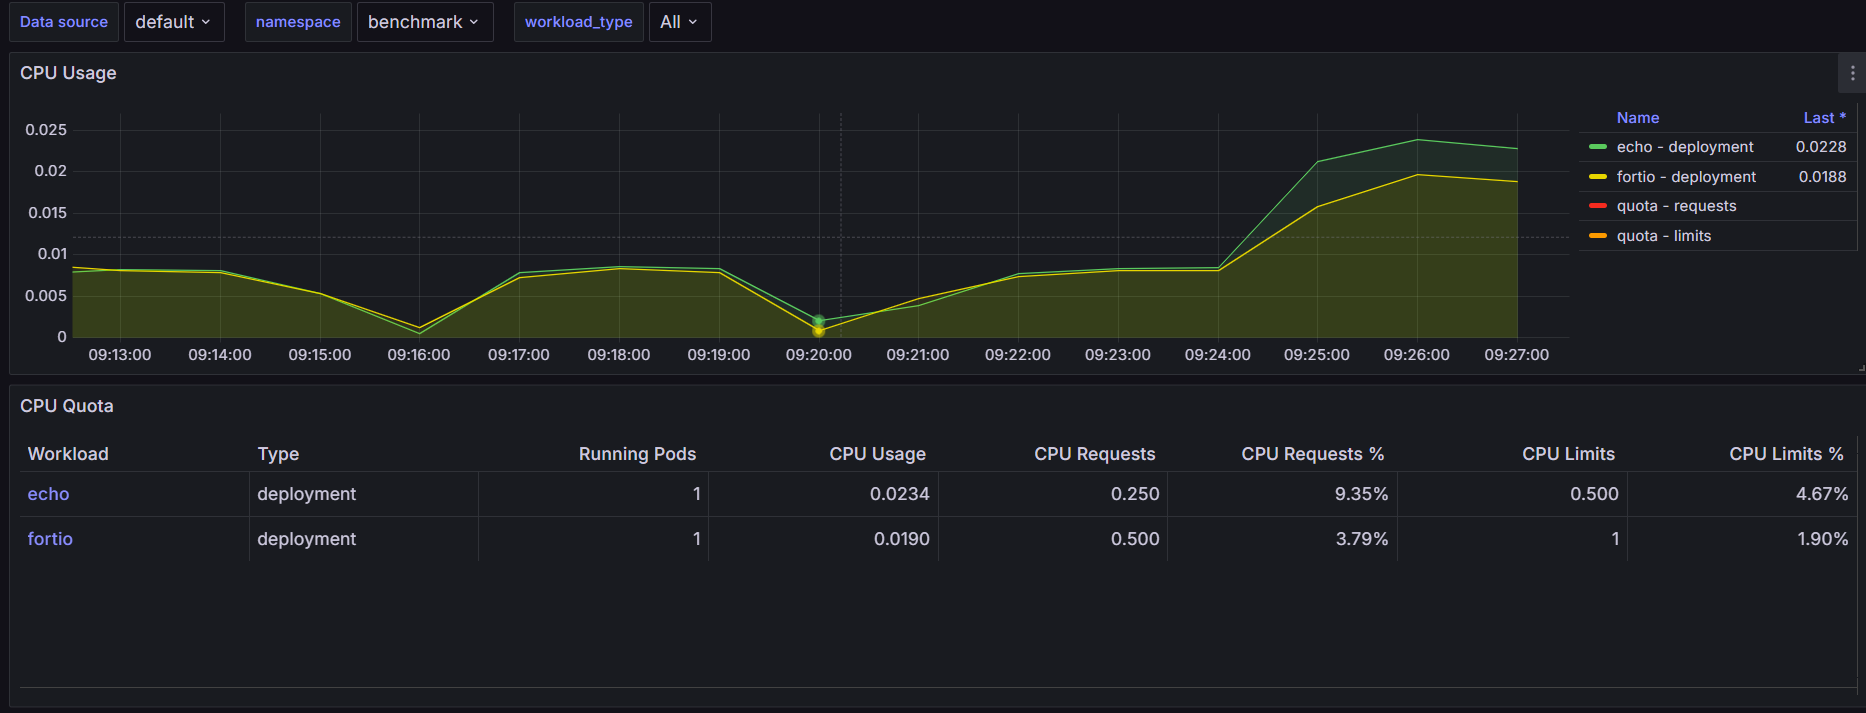
\includegraphics[width=0.92\textwidth]{../figures/grafana/modeA/grafana-ns-cpu-S1-L2-R1.png}
    \caption{Grafana bổ sung cho S1 L2 Mode A: CPU namespace}
    \label{fig:app-s1-l2-modea-cpu}
\end{figure}

\begin{figure}[H]
    \centering
    
\includegraphics[width=0.92\textwidth]{../figures/grafana/modeB/grafana-ns-cpu-S1-L2-R1.png}
    \caption{Grafana bổ sung cho S1 L2 Mode B: CPU namespace}
    \label{fig:app-s1-l2-modeb-cpu}
\end{figure}

\begin{figure}[H]
    \centering
    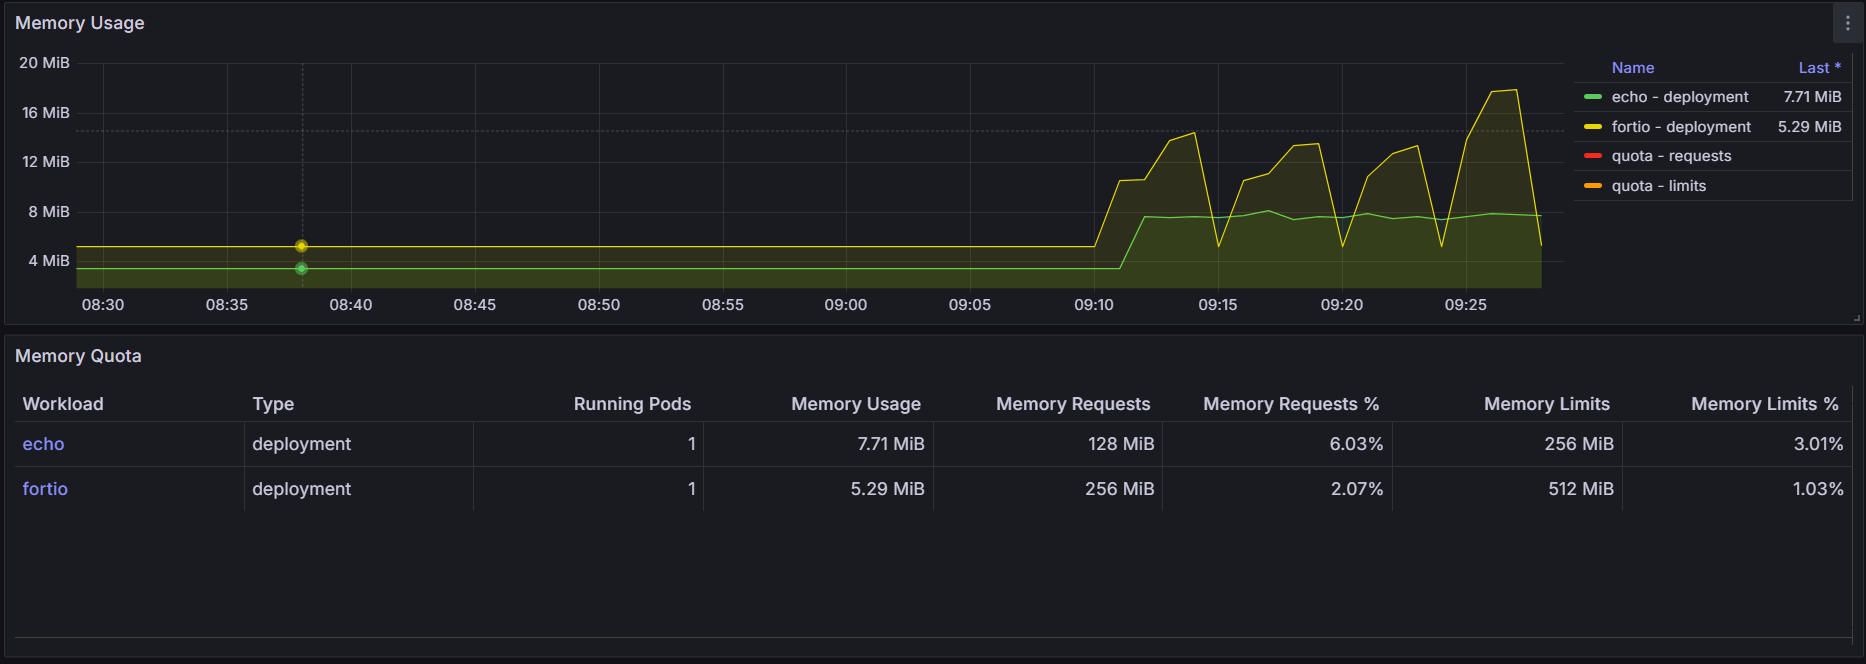
\includegraphics[width=0.92\textwidth]{../figures/grafana/modeA/grafana-ns-mem-S1-L2-R1.png}
    \caption{Grafana bổ sung cho S1 L2 Mode A: memory namespace}
    \label{fig:app-s1-l2-modea-memory}
\end{figure}

\begin{figure}[H]
    \centering
    
\includegraphics[width=0.92\textwidth]{../figures/grafana/modeB/grafana-ns-mem-S1-L2-R1.png}
    \caption{Grafana bổ sung cho S1 L2 Mode B: memory namespace}
    \label{fig:app-s1-l2-modeb-memory}
\end{figure}

\section{Ảnh Grafana bổ sung cho S2}

Các ảnh S2 L2 hỗ trợ đọc caveat của S2: biến động theo pha và churn cần được diễn giải thận trọng, thay vì quy trực tiếp cho resource pressure từ một ảnh dashboard.

\begin{figure}[H]
    \centering
    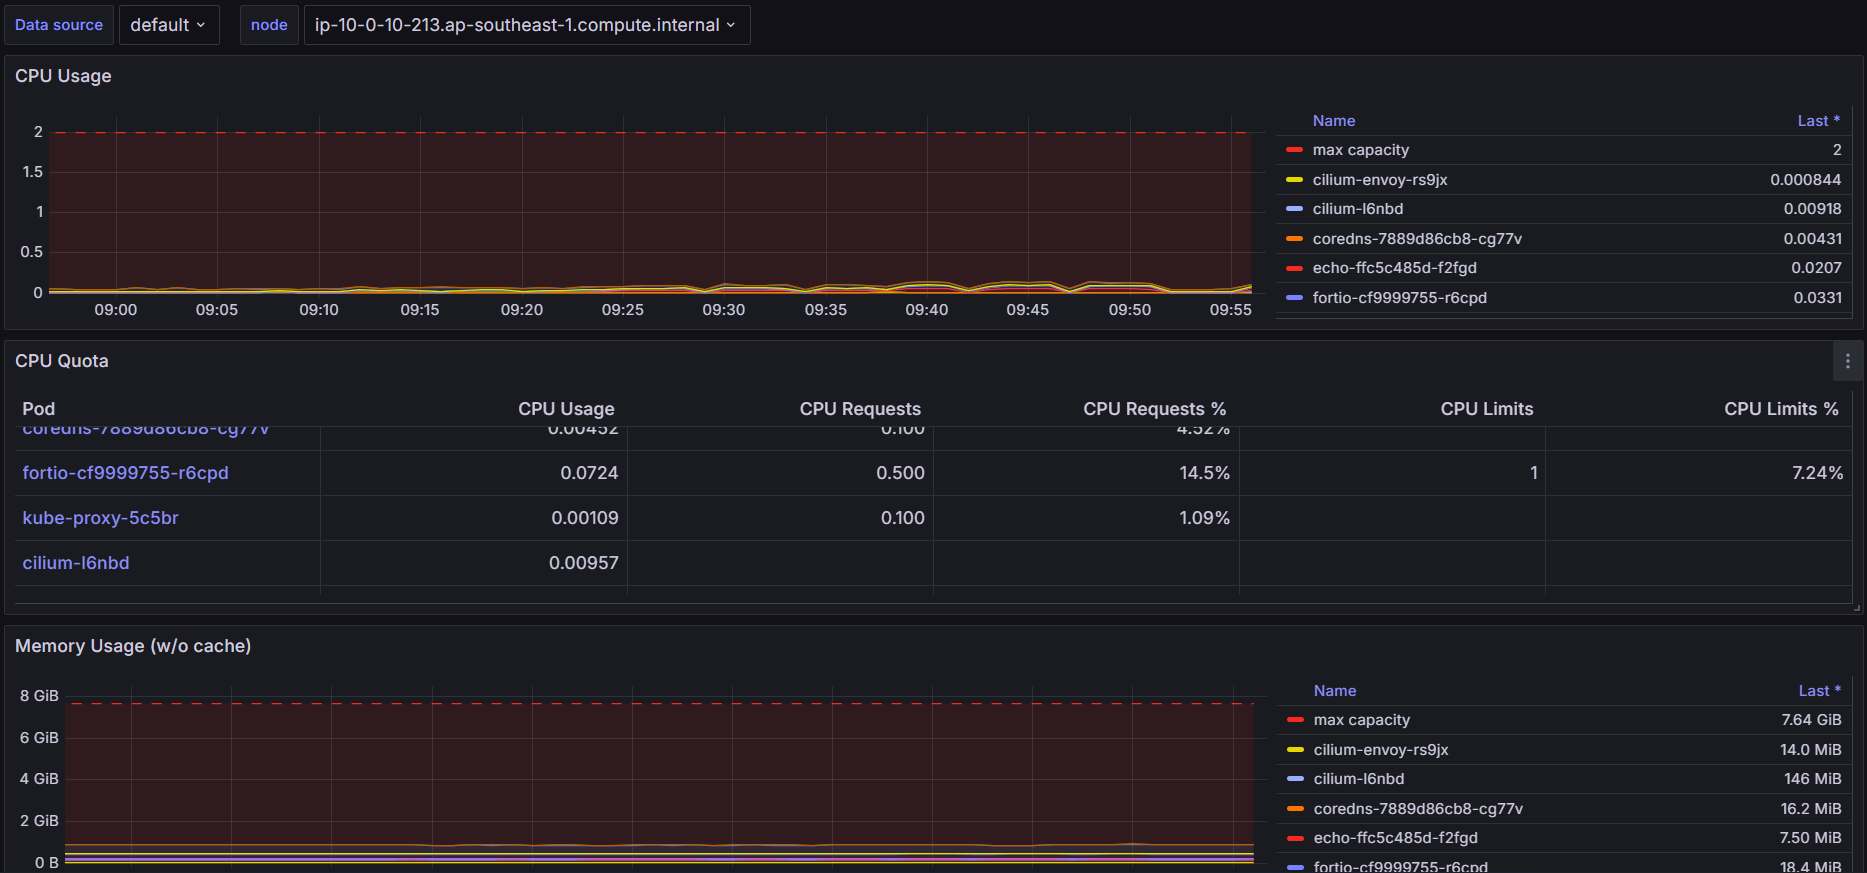
\includegraphics[width=0.92\textwidth]{../figures/grafana/modeA/grafana-node-cpu-mem-S2-L2-R1.png}
    \caption{Grafana bổ sung cho S2 L2 Mode A: node CPU/memory}
    \label{fig:app-s2-l2-modea-node-cpu-memory}
\end{figure}

\begin{figure}[H]
    \centering
    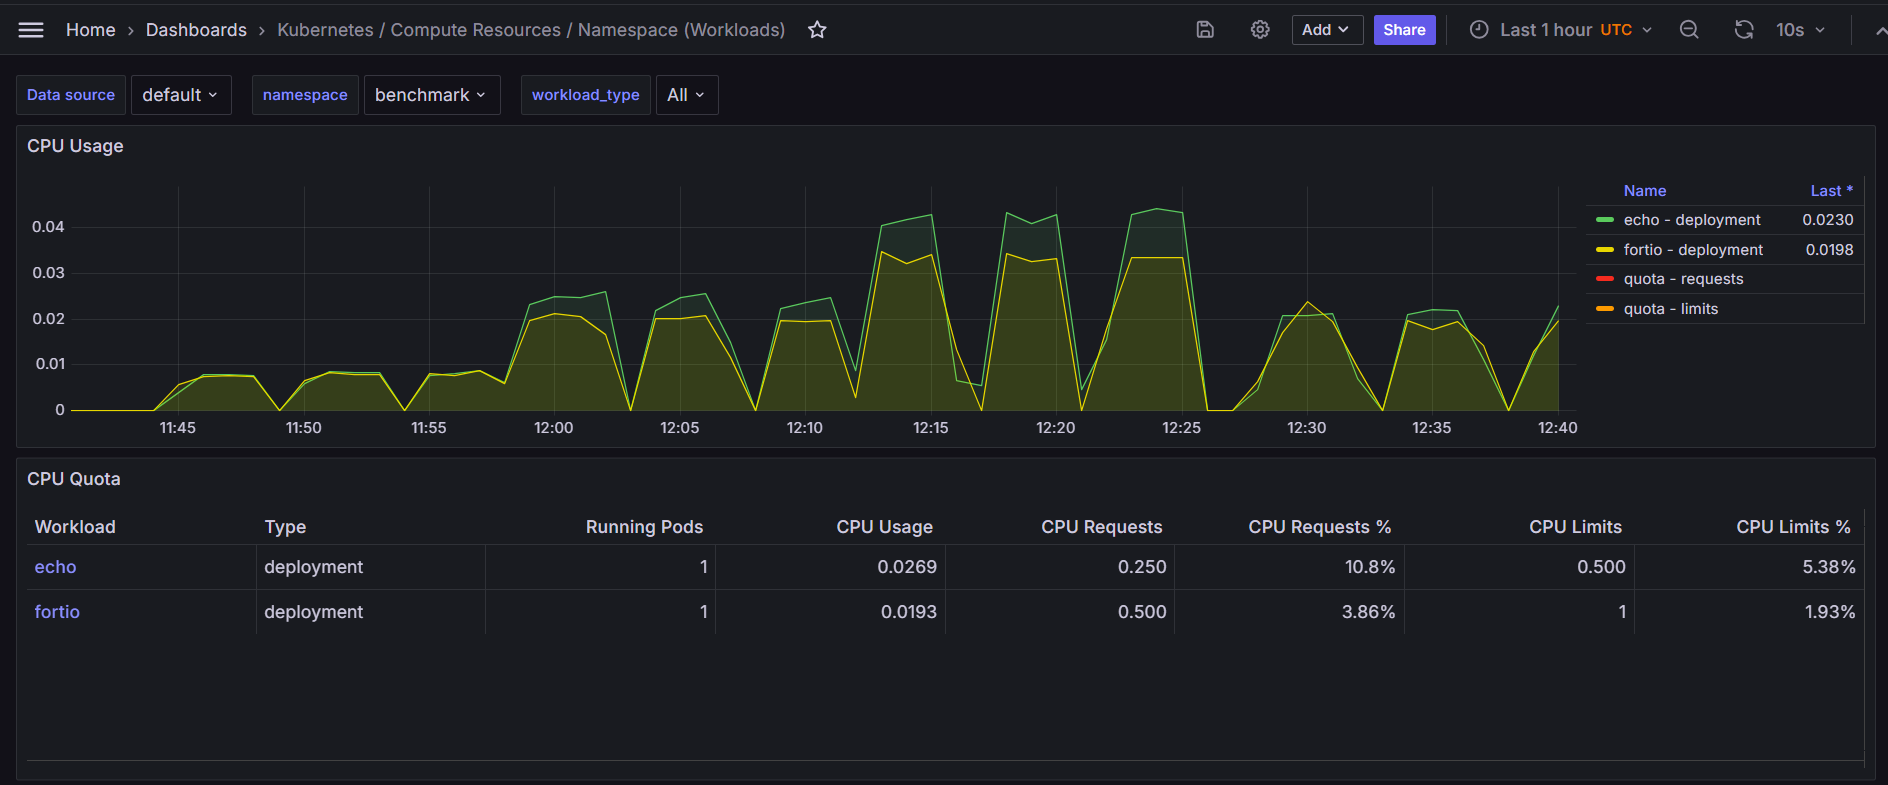
\includegraphics[width=0.92\textwidth]{../figures/grafana/modeB/grafana-ns-cpu-S2-L2.png}
    \caption{Grafana bổ sung cho S2 L2 Mode B: CPU namespace}
    \label{fig:app-s2-l2-modeb-cpu}
\end{figure}

\begin{figure}[H]
    \centering
    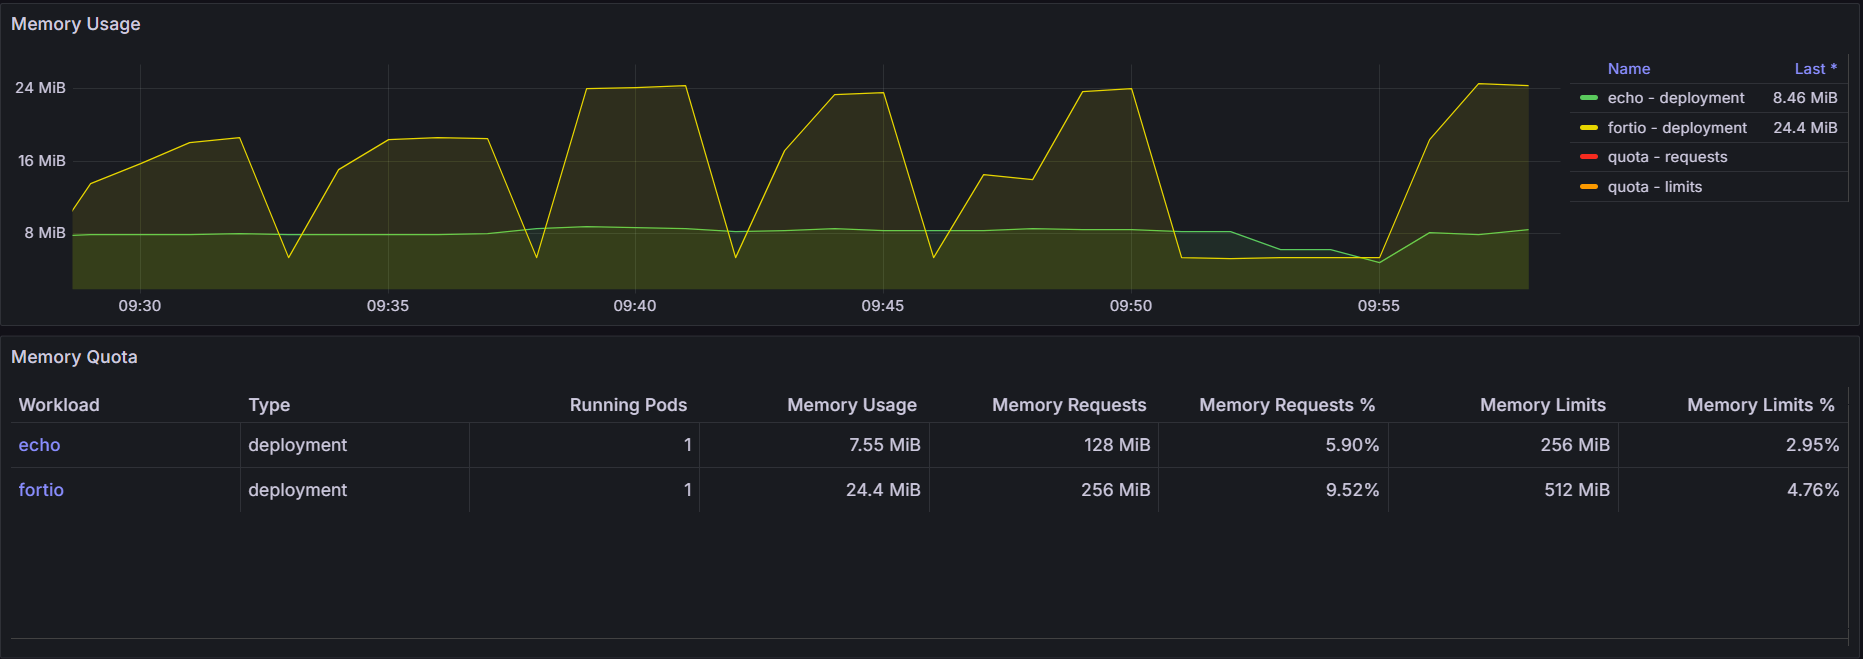
\includegraphics[width=0.92\textwidth]{../figures/grafana/modeA/grafana-ns-mem-S2-L2-R1.png}
    \caption{Grafana bổ sung cho S2 L2 Mode A: memory namespace}
    \label{fig:app-s2-l2-modea-memory}
\end{figure}

\begin{figure}[H]
    \centering
    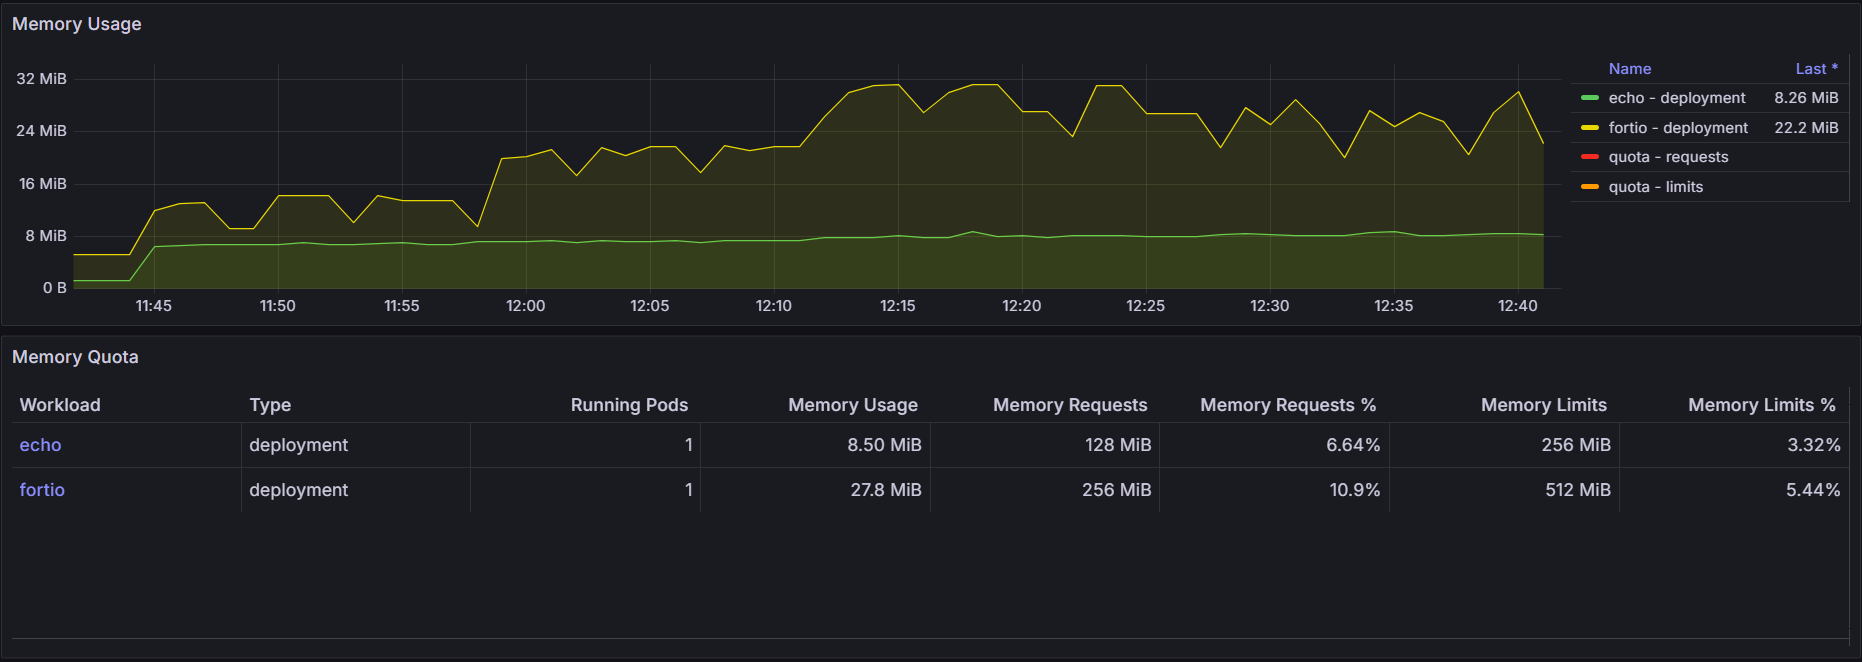
\includegraphics[width=0.92\textwidth]{../figures/grafana/modeB/grafana-ns-mem-S2-L2.png}
    \caption{Grafana bổ sung cho S2 L2 Mode B: memory namespace}
    \label{fig:app-s2-l2-modeb-memory}
\end{figure}

\section{Ảnh Grafana bổ sung cho S3}

S3 là kịch bản so sánh policy OFF/ON trong Mode B, không phải so sánh Mode A với Mode B. Các ảnh dưới đây hỗ trợ kiểm tra bối cảnh vận hành khi policy thay đổi. Chúng không được dùng để kết luận overhead bằng 0; kết luận ở Chương 4 vẫn dựa trên p99, RPS và error rate.

\begin{figure}[H]
    \centering
    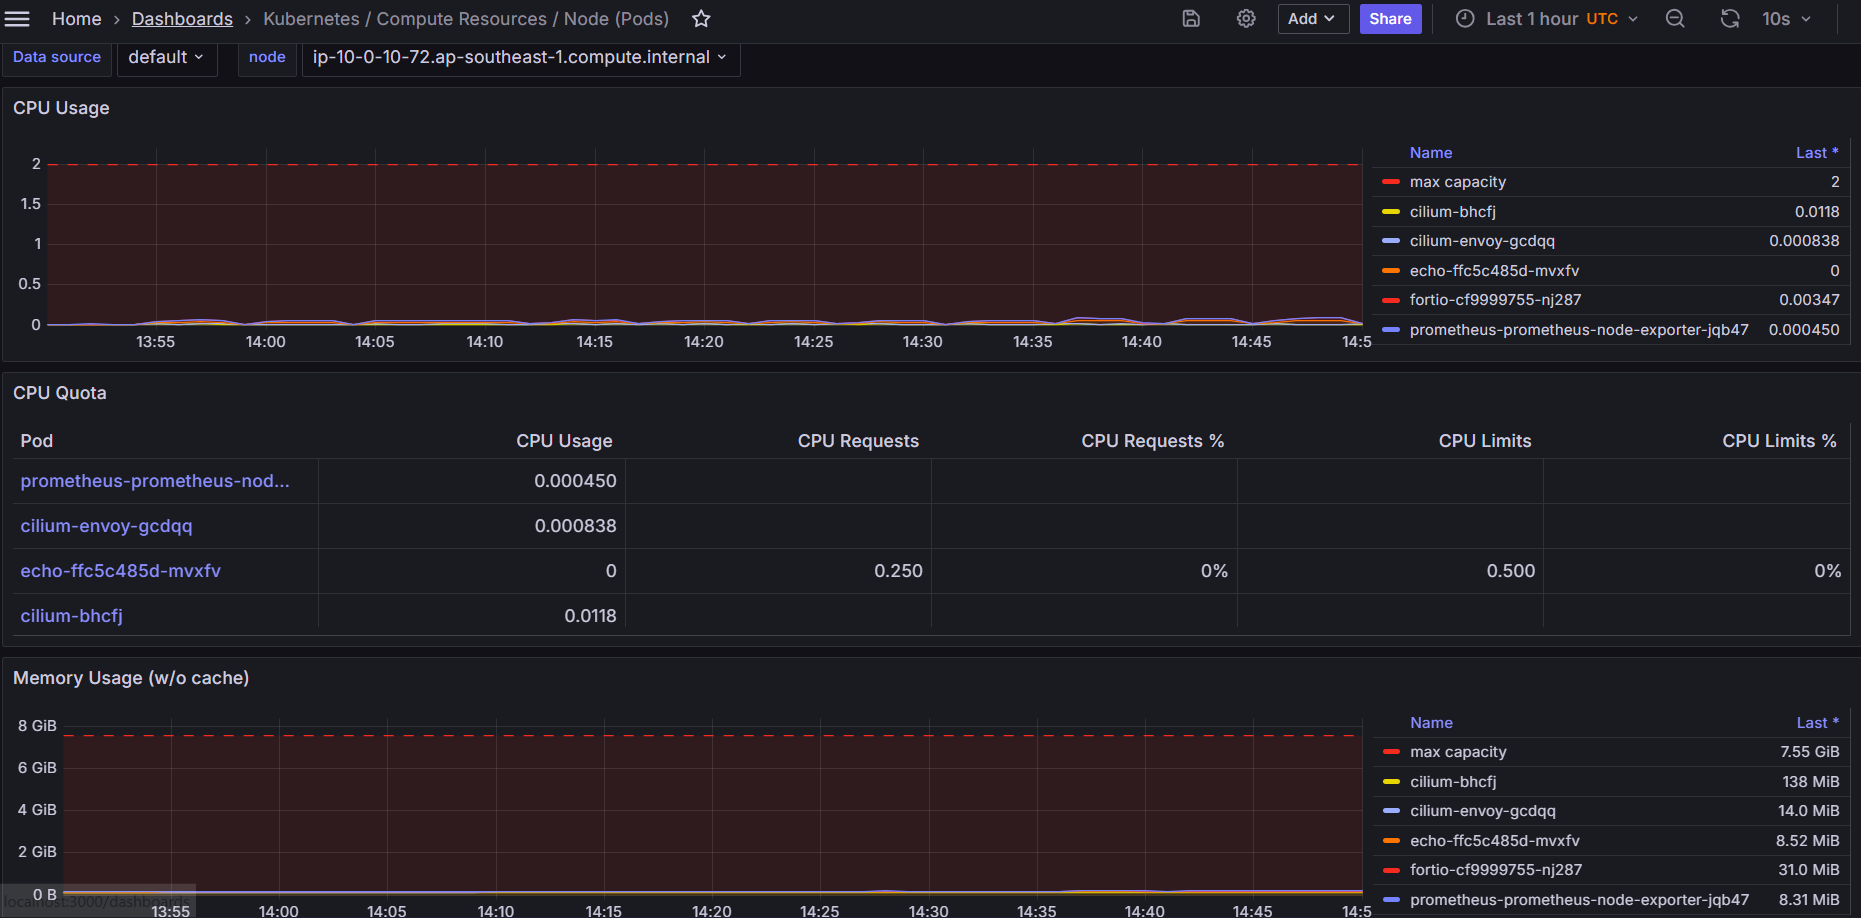
\includegraphics[width=0.92\textwidth]{../figures/grafana/modeB/grafana-ns-node-S3-off-L3.png}
    \caption{Grafana bổ sung cho S3 L3 trong Mode B: policy OFF}
    \label{fig:app-s3-l3-off-node}
\end{figure}

\begin{figure}[H]
    \centering
    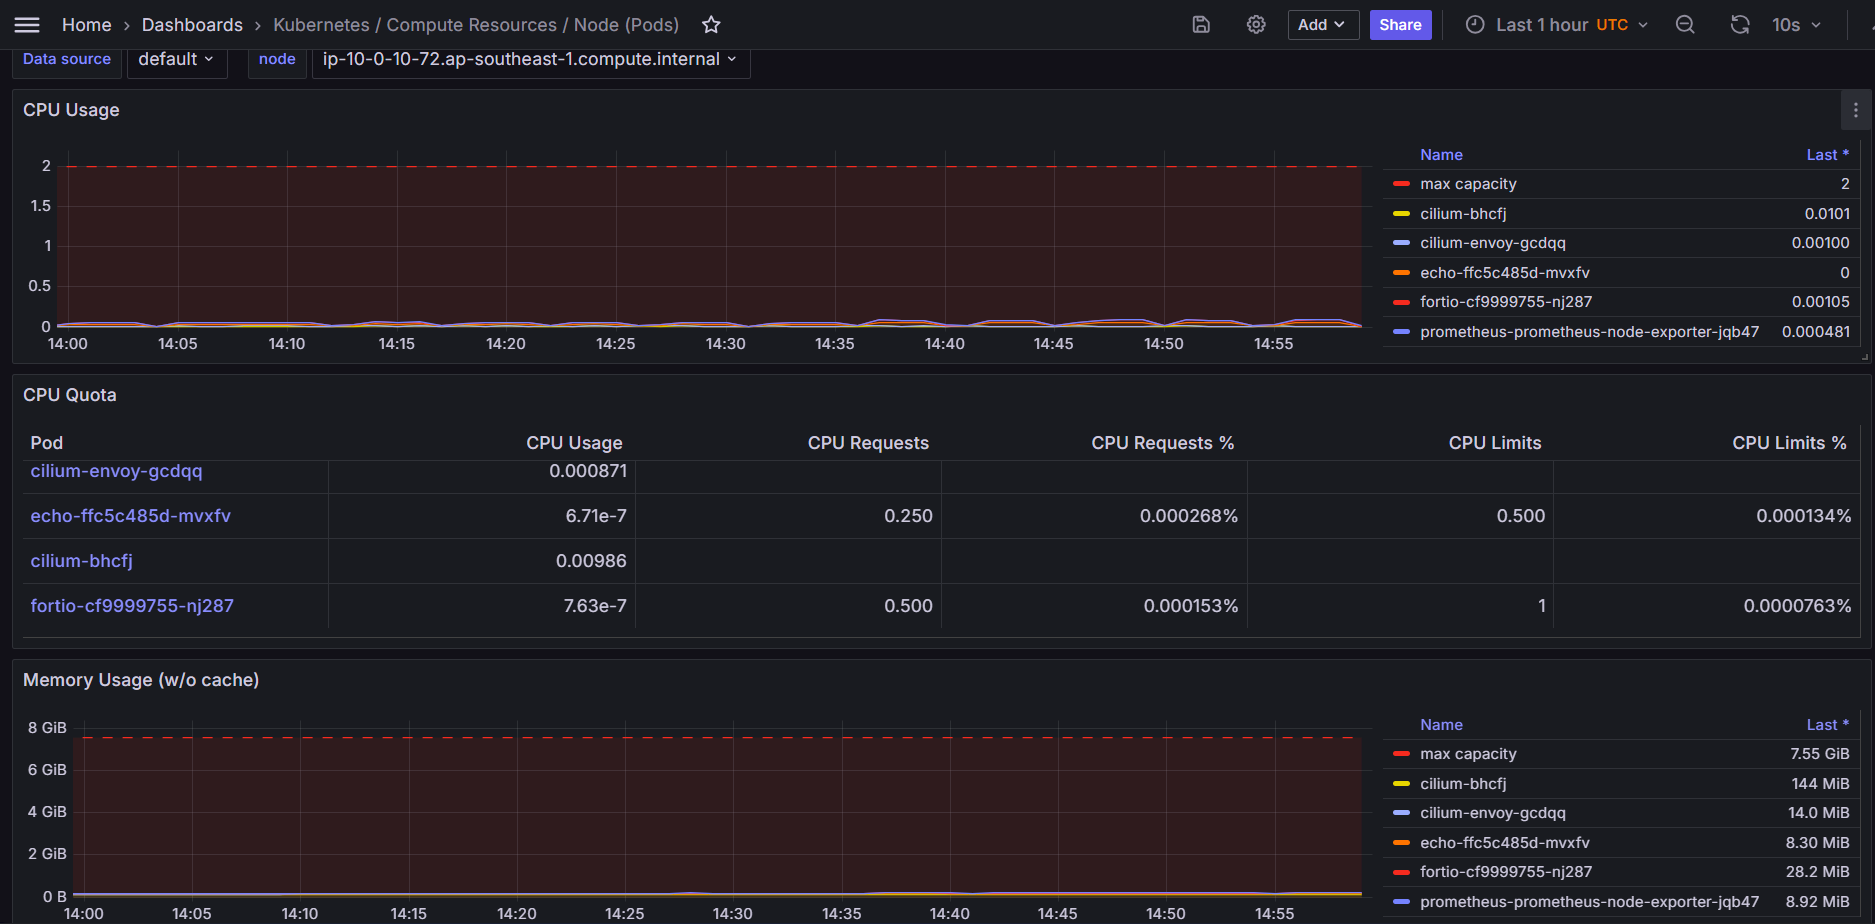
\includegraphics[width=0.92\textwidth]{../figures/grafana/modeB/grafana-ns-node-S3-on-L3.png}
    \caption{Grafana bổ sung cho S3 L3 trong Mode B: policy ON}
    \label{fig:app-s3-l3-on-node}
\end{figure}

\begin{figure}[H]
    \centering
    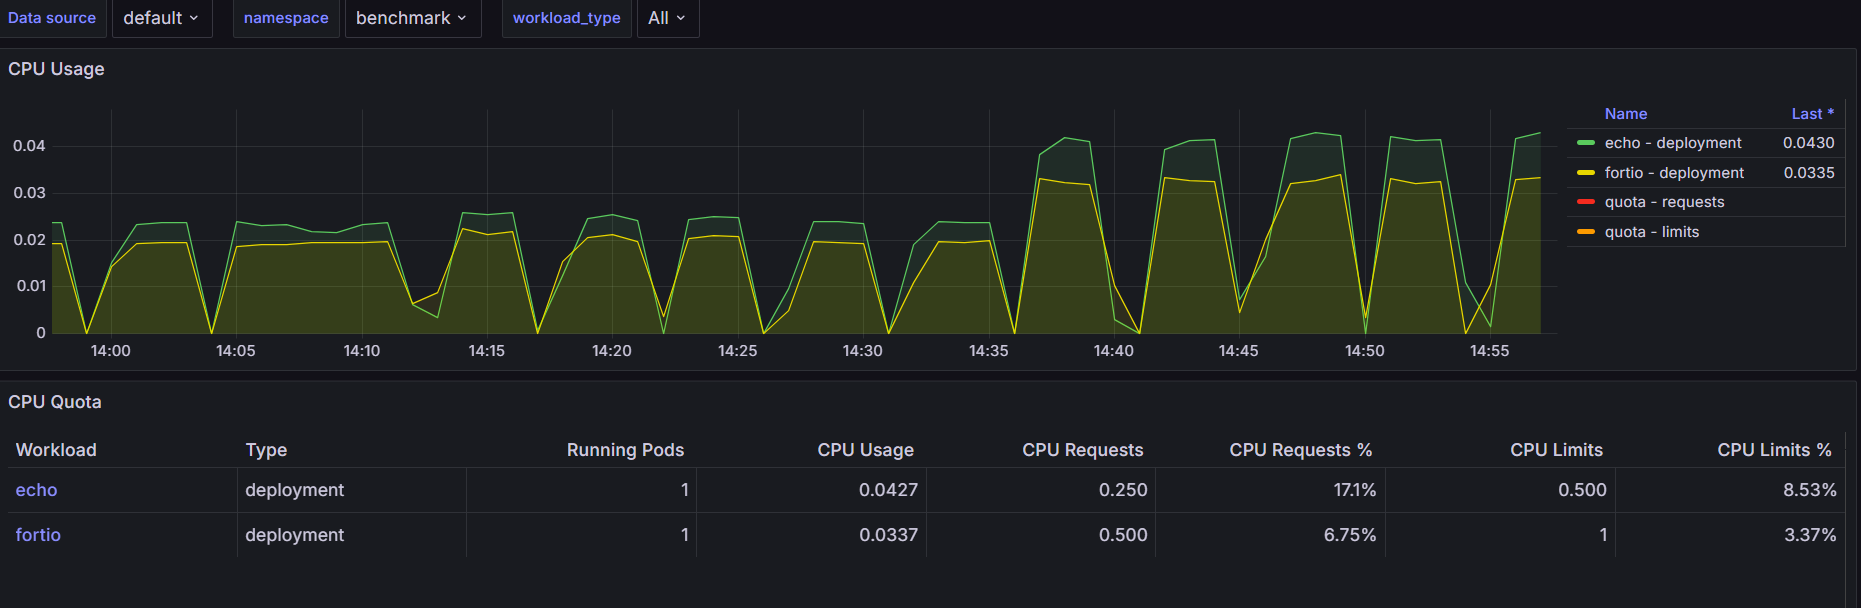
\includegraphics[width=0.92\textwidth]{../figures/grafana/modeB/grafana-ns-cpu-S3-on-L3.png}
    \caption{Grafana bổ sung cho S3 L3 policy ON: CPU namespace}
    \label{fig:app-s3-l3-on-cpu}
\end{figure}

\begin{figure}[H]
    \centering
    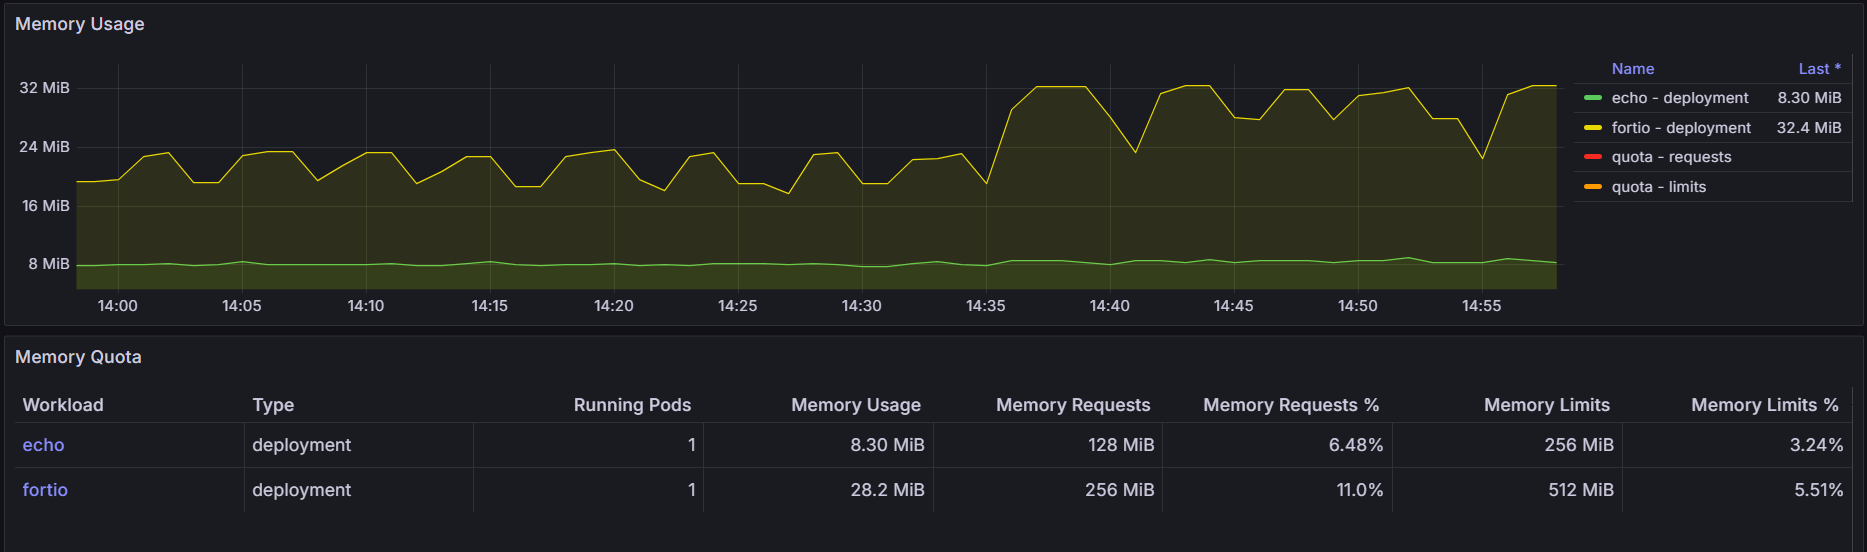
\includegraphics[width=0.92\textwidth]{../figures/grafana/modeB/grafana-ns-mem-S3-on-L3.png}
    \caption{Grafana bổ sung cho S3 L3 policy ON: memory namespace}
    \label{fig:app-s3-l3-on-memory}
\end{figure}

\section{Ảnh Hubble bổ sung}

Các ảnh Hubble dưới đây giúp minh họa thêm trạng thái Hubble, pod kiểm thử deny-case và màn hình chi tiết flow. Các ảnh này chỉ là evidence observability ở mức flow/verdict, không phải packet capture và không phải nguồn đo hiệu năng.

\begin{figure}[H]
    \centering
    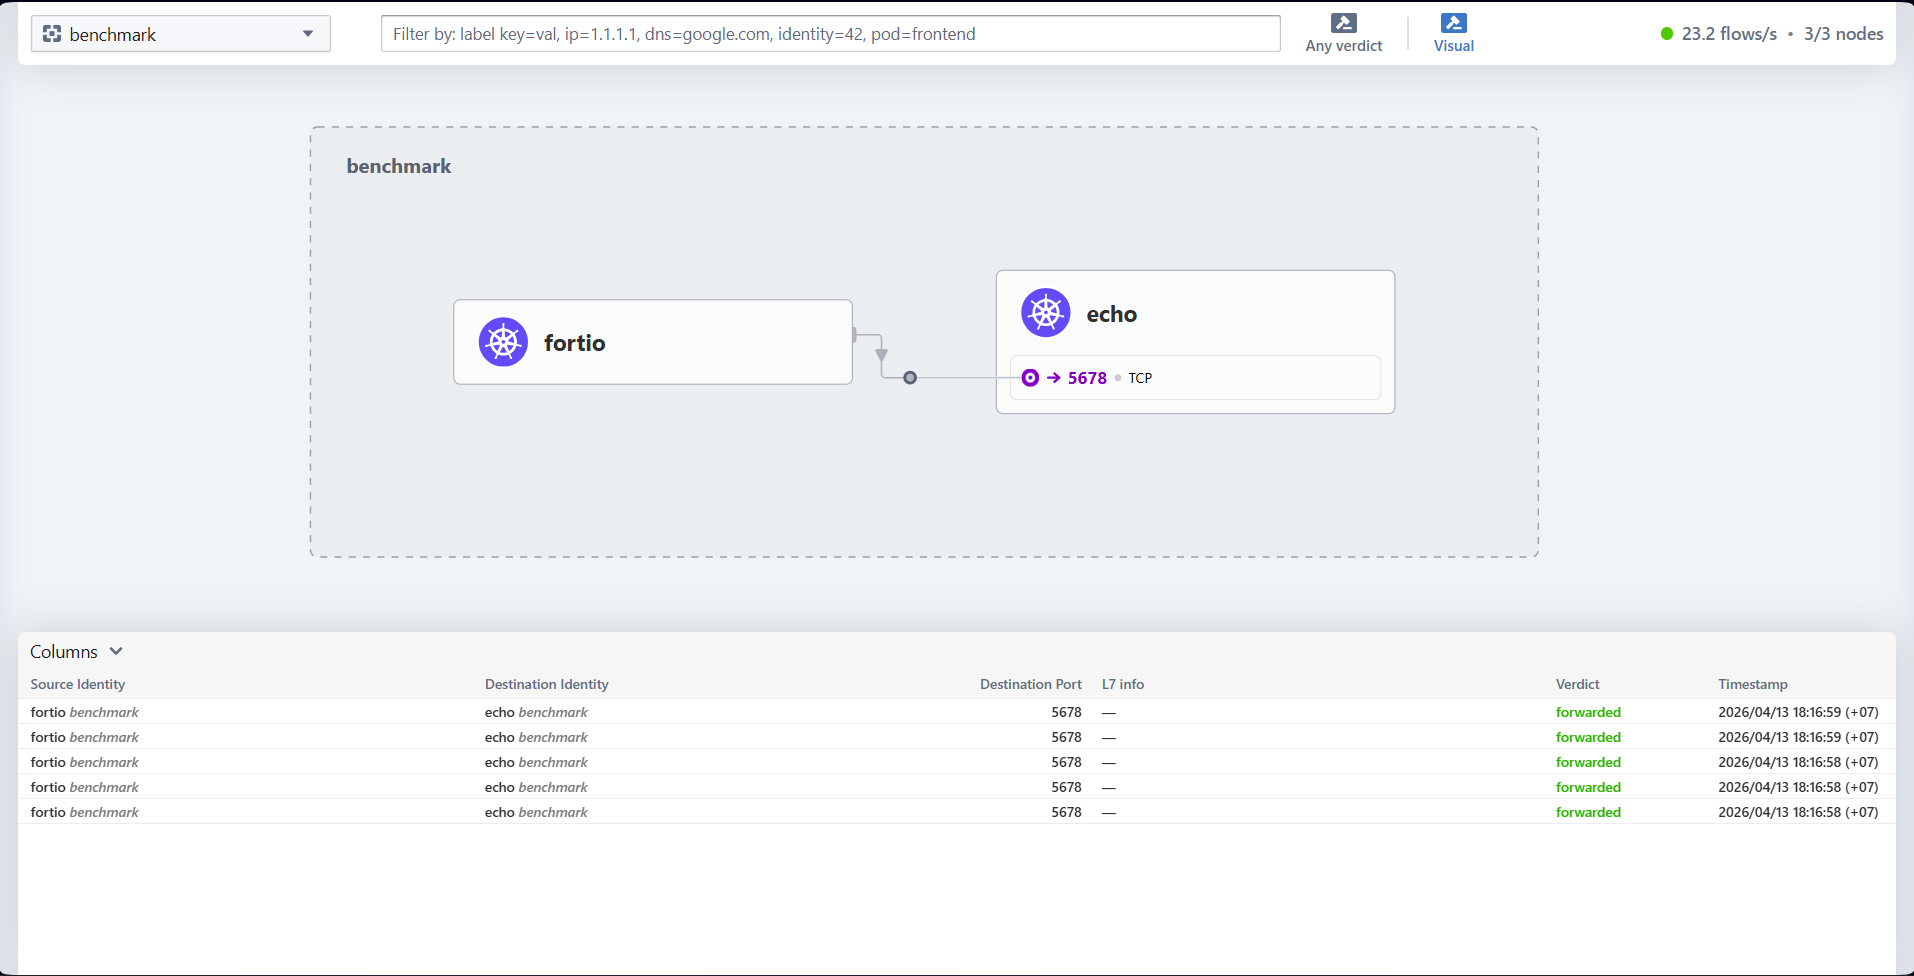
\includegraphics[width=0.92\textwidth]{../figures/hubble/fig-12-modeB-hubble-status.png}
    \caption{Ảnh Hubble bổ sung: trạng thái/flow Hubble trong Mode B}
    \label{fig:app-hubble-status}
\end{figure}

\begin{figure}[H]
    \centering
    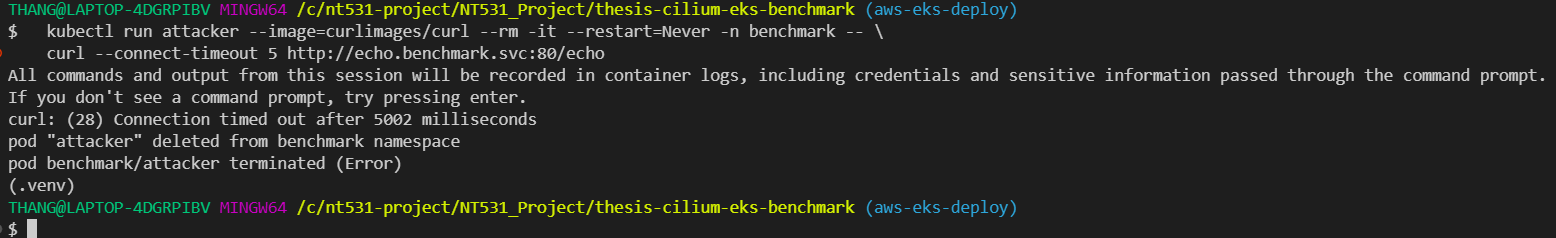
\includegraphics[width=0.92\textwidth]{../figures/hubble/fig-13-hubble-attacker-pod.png}
    \caption{Ảnh Hubble bổ sung: pod dùng cho manual deny-case}
    \label{fig:app-hubble-attacker-pod}
\end{figure}

\begin{figure}[H]
    \centering
    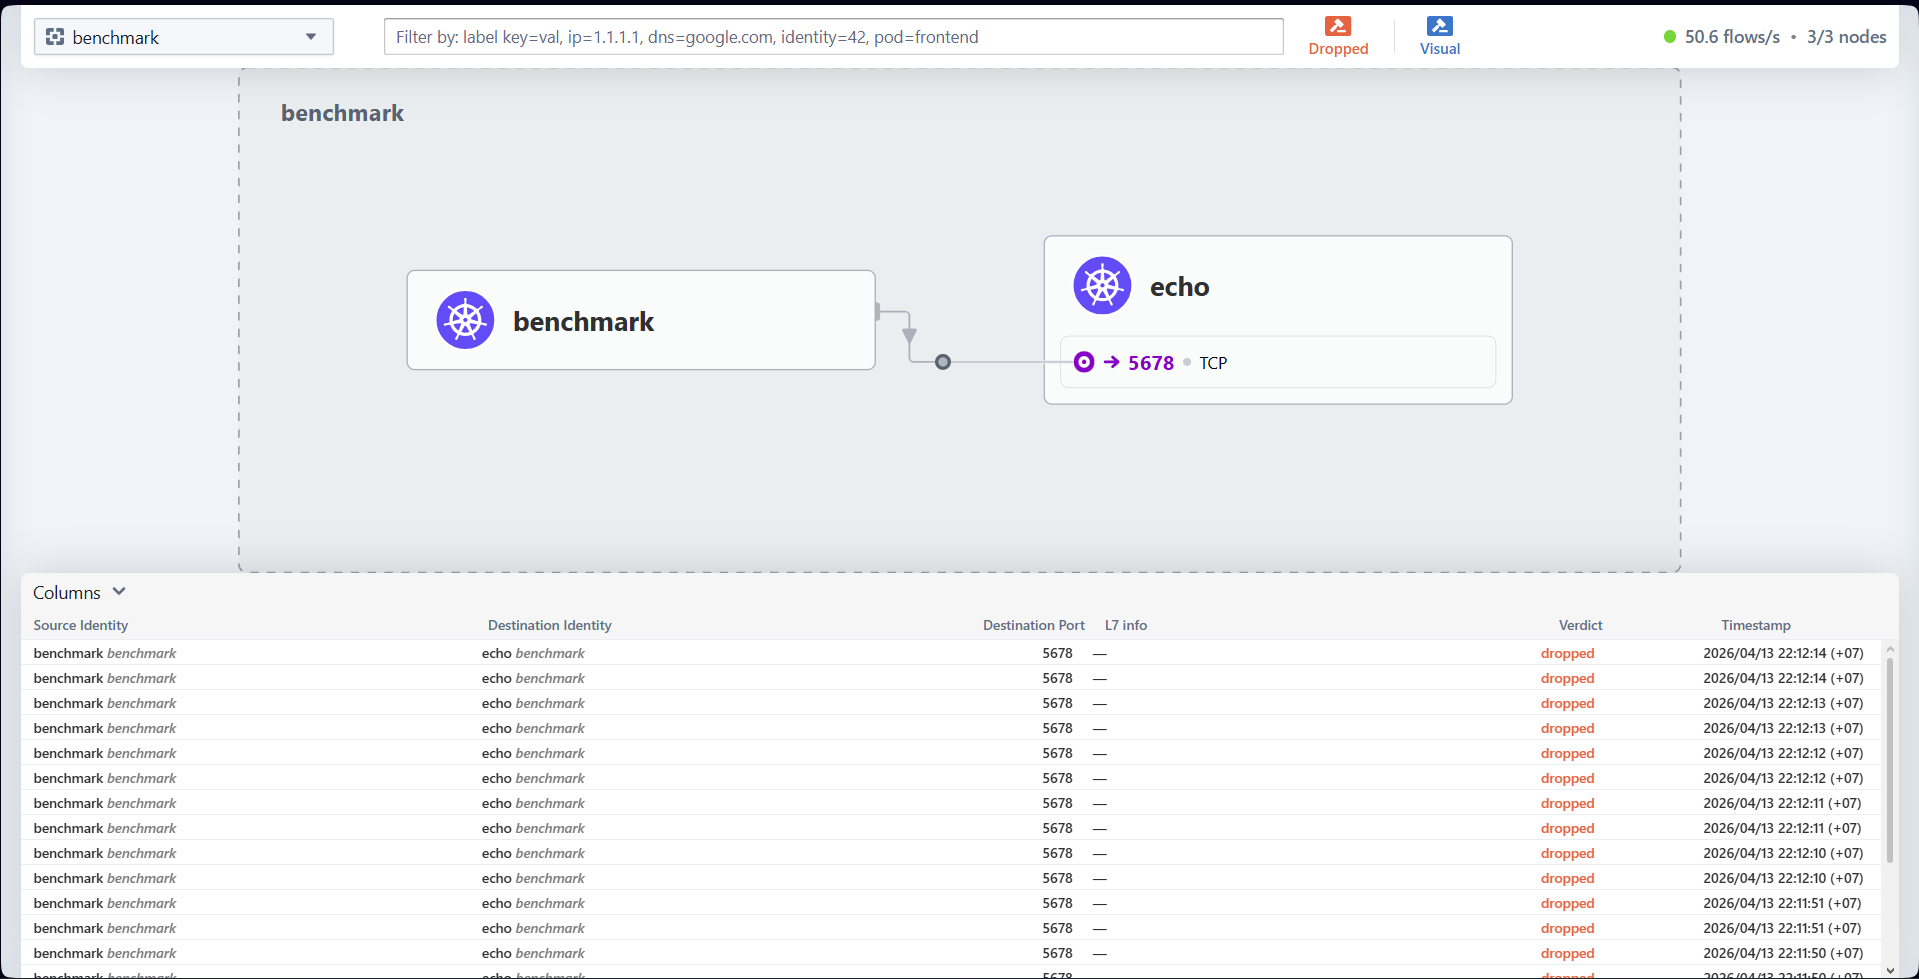
\includegraphics[width=0.92\textwidth]{../figures/hubble/fig-13-hubble-deny-case.png}
    \caption{Ảnh Hubble bổ sung: deny-case ở mức overview}
    \label{fig:app-hubble-deny-overview}
\end{figure}

\begin{figure}[H]
    \centering
    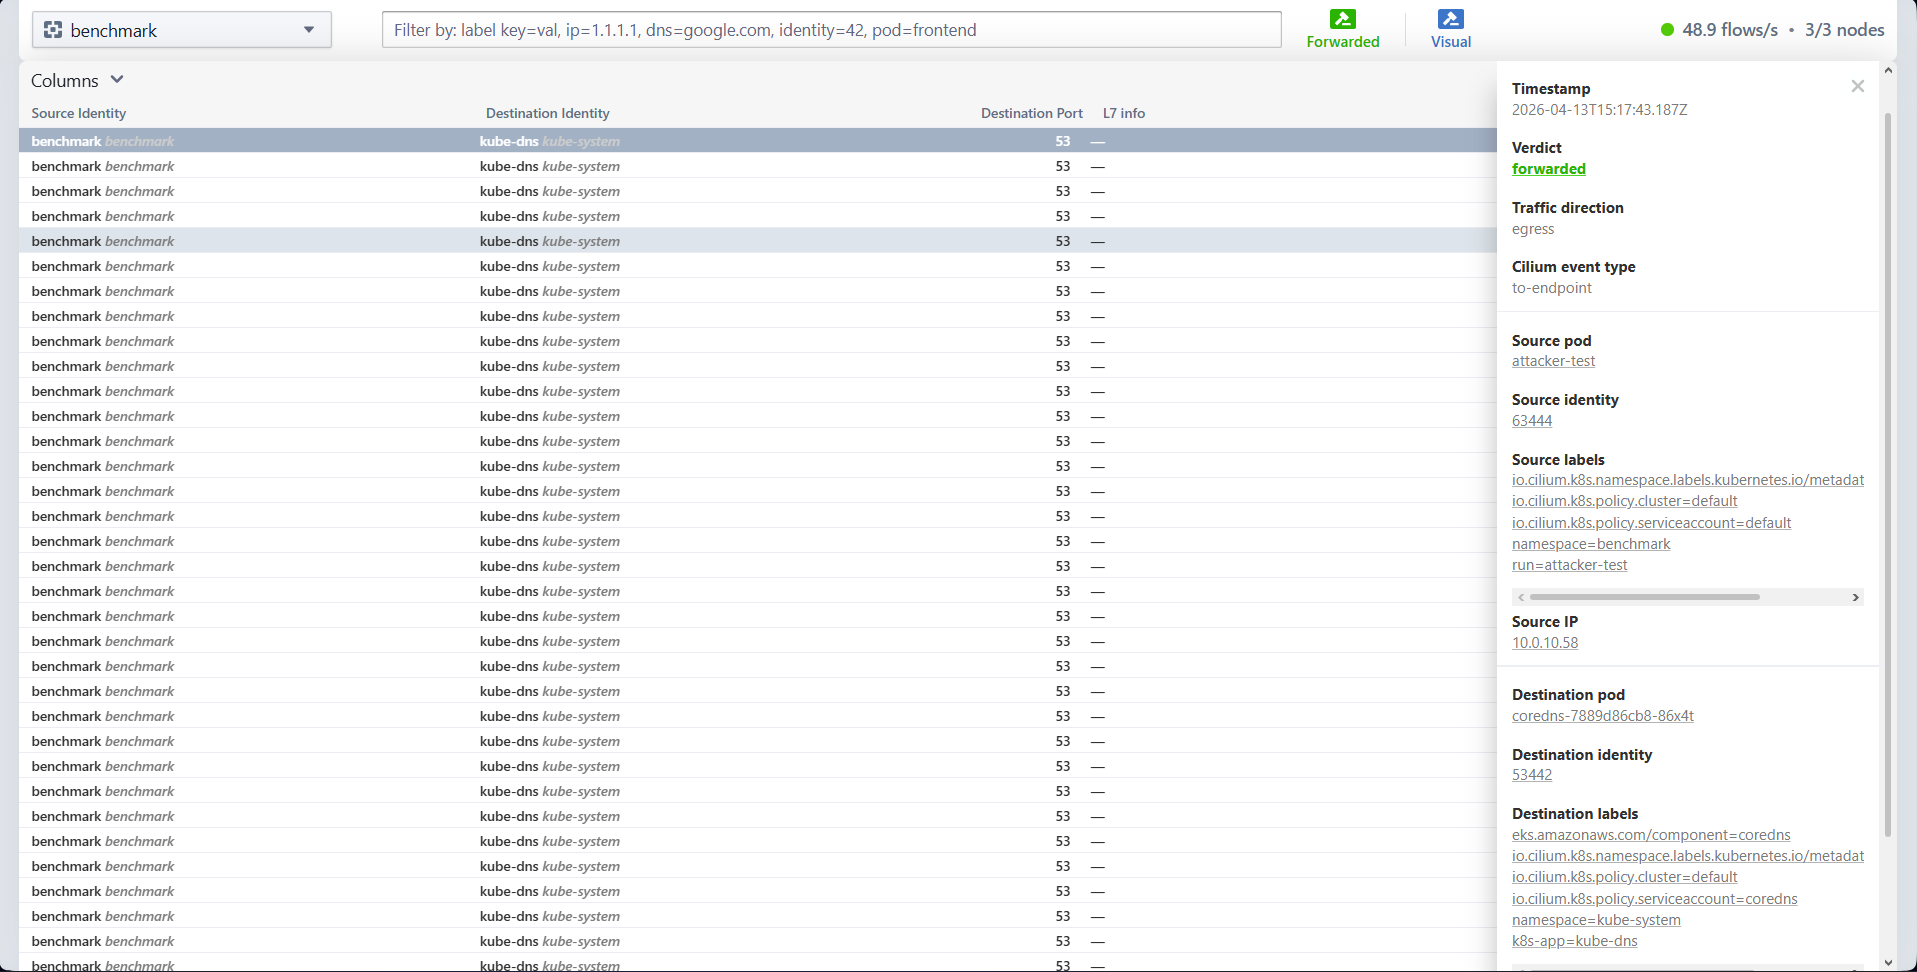
\includegraphics[width=0.92\textwidth]{../figures/hubble/fig-13b-hubble-forwarded-case-detail.png}
    \caption{Ảnh Hubble bổ sung: chi tiết một forwarded flow}
    \label{fig:app-hubble-forwarded-detail}
\end{figure}

% !TeX root = ../main.tex
% Phụ lục F - Scripts va cau hinh thuc nghiem

\chapter{Phụ lục F: Kịch bản và cấu hình thí nghiệm (Scripts \& Configuration)}
\label{app:scripts-config}

Phụ lục này mô tả các script và manifest cấu hình dùng trong pipeline benchmark. Mục tiêu là minh bạch cách tự động hóa chạy thí nghiệm, thu thập bằng chứng và phân tích dữ liệu, hạn chế tối đa thao tác thủ công dễ sai sót.
\section{ Liên kết mã nguồn đầy đủ}

Kho mã nguồn gốc của dự án được lưu tại:

\begin{center}
\url{https://github.com/daithang59/NT531_EKS-Cilium-Kubeproxy-Benchmark/tree/main/scripts}
\end{center}
\section{Các kịch bản chạy Benchmark (Benchmark Scripts)}

Phần này liệt kê các script Bash chịu trách nhiệm ép tải và thu thập artifact theo Results Contract.

\begin{itemize}
		\item \texttt{scripts/calibrate.sh}: chạy calibration sweep để xác định các mốc tải L1, L2, L3 dựa trên dữ liệu thực đo trước khi chạy benchmark chính thức.
		\item \texttt{scripts/run\_s1.sh}: chạy benchmark steady-state với tải cố định để đo baseline latency/throughput qua ClusterIP Service.
		\item \texttt{scripts/run\_s2.sh}: chạy benchmark nhiều pha (ramp-up, sustained, burst, cooldown) và tạo connection churn bằng \texttt{keepalive=false}.
		\item \texttt{scripts/run\_s3.sh}: chạy benchmark theo hai pha policy OFF/ON để đo overhead của NetworkPolicy enforcement.
		\item \texttt{scripts/collect\_meta.sh} và \texttt{scripts/collect\_hubble.sh}: thu thập metadata cụm, trạng thái datapath, và flow logs từ Hubble làm bằng chứng kiểm chứng.
\end{itemize}

\textbf{Snippet trọng tâm từ \texttt{scripts/run\_s1.sh}:}

\begin{lstlisting}[language=bash]
set -euo pipefail

export SCENARIO="S1"
source "$(dirname "$0")/common.sh"

preflight_checks

for i in $(seq 1 "${REPEAT}"); do
	execute_run "${i}"

	# Rest between runs (skip after last)
	if [[ "${i}" -lt "${REPEAT}" ]]; then
		sleep "${REST_BETWEEN_RUNS}"
	fi
done
\end{lstlisting}

Snippet S1 cho thấy vòng lặp lặp lại \texttt{REPEAT}, gọi \texttt{execute\_run} để chạy Fortio và thu thập artifact cho từng run.

\textbf{Snippet trọng tâm từ \texttt{scripts/run\_s2.sh}:}

\begin{lstlisting}[language=bash]
set -euo pipefail

export SCENARIO="S2"
source "$(dirname "$0")/common.sh"

preflight_checks

# Derived QPS levels for phases
QPS_50PCT=$(( BENCH_QPS / 2 ))
QPS_150PCT=$(( BENCH_QPS * 3 / 2 ))
CONNS_HIGH=$(( BENCH_CONNS * 2 ))

# Phase durations
RAMP_SEC="${S2_RAMP_SEC:-30}"
SUSTAINED_SEC="${S2_SUSTAINED_SEC:-90}"
BURST_SEC="${S2_BURST_SEC:-20}"
BURST_COUNT="${S2_BURST_COUNT:-3}"
BURST_REST="${S2_BURST_REST:-10}"
COOLDOWN_SEC="${S2_COOLDOWN_SEC:-30}"

for run_num in $(seq 1 "${REPEAT}"); do
	outdir="$(make_outdir "${run_num}")"
	write_metadata "${outdir}" "${run_num}"
	collect_meta "${outdir}"

	# ---- Phase 1: Ramp-up (50% QPS) ------------------------------------------
	_fortio_rest "${outdir}" "phase1_rampup" "${QPS_50PCT}" "${BENCH_CONNS}" "${RAMP_SEC}"
	# ---- Phase 2: Sustained high (100% QPS, 2x connections) ------------------
	_fortio_rest "${outdir}" "phase2_sustained" "${BENCH_QPS}" "${CONNS_HIGH}" "${SUSTAINED_SEC}"

	# ---- Phase 3: Bursts (150% QPS x N, with rest between) -------------------
	for b in $(seq 1 "${BURST_COUNT}"); do
		_fortio_rest "${outdir}" "phase3_burst${b}" "${QPS_150PCT}" "${CONNS_HIGH}" "${BURST_SEC}"
		if [[ "${b}" -lt "${BURST_COUNT}" ]]; then
			sleep "${BURST_REST}"
		fi
	done

	# ---- Phase 4: Cool-down (50% QPS) ----------------------------------------
	_fortio_rest "${outdir}" "phase4_cooldown" "${QPS_50PCT}" "${BENCH_CONNS}" "${COOLDOWN_SEC}"
	# ---- Combine all phase logs into bench.log --------------------------------
	cat "${outdir}"/bench_phase*.log > "${outdir}/bench.log"
	# ---- Post-run evidence ----------------------------------------------------
	collect_cilium_hubble "${outdir}"
	write_checklist "${outdir}" "${run_num}"
done
\end{lstlisting}

Snippet S2 thể hiện rõ logic chạy đa pha và tổng hợp log pha về \texttt{bench.log} để phân tích thống nhất.

\textbf{Snippet trọng tâm từ \texttt{scripts/run\_s3.sh} (giữ comment logic chính):}

\begin{lstlisting}[language=bash]
set -euo pipefail

# If script exits unexpectedly, always remove policies to avoid side effects.
cleanup_s3_policies() {
		kubectl -n "${NS}" delete -f "${REPO_ROOT}/workload/policies/" \
				--ignore-not-found=true >/dev/null 2>&1 || true
}
trap cleanup_s3_policies EXIT INT TERM

export SCENARIO="S3"
source "$(dirname "$0")/common.sh"

preflight_checks

# ---------- Phase OFF: remove policies ----------------------------------------
kubectl -n "${NS}" delete -f "${REPO_ROOT}/workload/policies/" --ignore-not-found=true
sleep 15

for i in $(seq 1 "${REPEAT}"); do
	export OUTDIR="${REPO_ROOT}/results/mode=${MODE_LABEL}/scenario=${SCENARIO}/load=${LOAD}/phase=off/run=R${i}_$(ts_dir)"
	# No policy active in phase=off
	unset POLICY_METADATA
	execute_run "${i}"
done
unset OUTDIR

# ---------- Phase ON: apply policies -----------------------------------------
kubectl apply -f "${REPO_ROOT}/workload/policies/"
sleep 20

POLICY_COUNT=$(find "${REPO_ROOT}/workload/policies/" -name "*.yaml" 2>/dev/null | wc -l | tr -d ' ')
export POLICY_METADATA="enabled=true,type=CiliumNetworkPolicy,complexity_level=simple,rule_count_estimate=${POLICY_COUNT}"

for i in $(seq 1 "${REPEAT}"); do
	export OUTDIR="${REPO_ROOT}/results/mode=${MODE_LABEL}/scenario=${SCENARIO}/load=${LOAD}/phase=on/run=R${i}_$(ts_dir)"
	execute_run "${i}"
done
unset OUTDIR
unset POLICY_METADATA

# ---------- Cleanup: remove policies after S3 completes ----------------------
kubectl -n "${NS}" delete -f "${REPO_ROOT}/workload/policies/" --ignore-not-found=true
\end{lstlisting}

Snippet S3 minh họa chu trình OFF $\rightarrow$ ON của policy và cơ chế \texttt{trap} để dọn policy khi script thoát bất thường.

\section{Các kịch bản phân tích dữ liệu (Analysis Scripts)}

Đây là các script Python xử lý dữ liệu thô thành kết quả cuối cùng, đảm bảo toàn bộ phép tính được tự động hóa và có thể tái lập.

\begin{itemize}
		\item \texttt{scripts/analyze\_results.py}: đọc artifact benchmark, parse log Fortio, tổng hợp thống kê theo nhóm (mode/scenario/load/phase), xuất \texttt{aggregated\_summary.csv} và \texttt{comparison\_AB.csv}; đồng thời thực hiện kiểm định Welch's t-test, tính \(p\)-value và \(\Delta\%\).
		\item \texttt{scripts/generate\_charts.py}: đọc CSV phân tích và tự động sinh toàn bộ biểu đồ phục vụ đồ án (định dạng PNG/PDF), bao gồm nhóm biểu đồ S1/S2/S3, repeatability và calibration.
\end{itemize}

\section{Các file cấu hình Workload và Policy (Workload Manifests)}

Phần này mô tả các manifest YAML dùng để triển khai workload benchmark trên Kubernetes và policy cho kịch bản S3.

\begin{itemize}
		\item \texttt{workload/server/01-namespace.yaml}: khởi tạo namespace \texttt{benchmark} cho workload đo đạc.
		\item \texttt{workload/server/02-echo-deploy.yaml}: triển khai HTTP echo server với cấu hình tài nguyên cố định để giảm nhiễu khi đo.
		\item \texttt{workload/server/03-echo-svc.yaml}: khai báo ClusterIP Service làm đích truy cập cho Fortio.
		\item \texttt{workload/client/01-fortio-deploy.yaml}: triển khai pod Fortio chạy chế độ server/runner để phát sinh tải benchmark.
		\item \texttt{workload/policies/01-cilium-policy-allow-fortio-to-echo.yaml} và \texttt{workload/policies/02-cilium-policy-deny-other.yaml}: định nghĩa CiliumNetworkPolicy dùng cho pha ON của S3 để kiểm tra overhead enforcement và hành vi allow/deny.
		\item \texttt{helm/cilium/values-baseline.yaml} và \texttt{helm/cilium/values-ebpfkpr.yaml}: hai file Helm values tạo khác biệt datapath giữa Mode A (\texttt{kubeProxyReplacement: false}) và Mode B (\texttt{kubeProxyReplacement: true}).
\end{itemize}



\end{document}
